\chapter{Event Selection}
\label{ch:event_selection}



This chapter describes the event selection applied to the data samples 
to reject background events, while keeping a significant number of selected $\nu_\mu$ \acrshort{cc} events.
Since the probability of having two or more neutrino interactions per beam spill is small, the selection aims to select one or zero neutrino candidate interactions per event, together with the muon candidate track.
The signal definition for this analysis is $\nu_\mu$ \acrshort{cc}, and all the distributions shown in this chapter that are labeled as ``signal'' show the distribution of $\nu_\mu$ \acrshort{cc} simulated events. The event selection, that acts on reconstructed variables, aims to get a $\nu_\mu$ \acrshort{cc} enriched sample by requiring at least one muon in the final state. 
An overview of the selection is shown in Figure~\ref{fig:evt_sel_overview}. The selection starts by requiring optical activity in the beam spill window (Section~\ref{sec:beam_spill}). Then, all the reconstructed interactions in the event are collected and a flash matching between such interactions and  the candidate neutrino flash is performed to select zero or one interaction per event (Section~\ref{sec:selection_fm}). In the events where one neutrino candidate is selected, the muon is identified (Section~\ref{sec:selection_muon_candidate}) and a series of quality cuts are applied to guarantee that the muon is well reconstructed (Sections~\ref{sec:selection_quality}). The interaction is then required to have the vertex inside the \acrshort{fv} to be selected (Section~\ref{sec:fiducial_volume}).
Finally, the selected event distributions are shown in Section~\ref{sec:event_distributions}, and the event selection performances in Section~\ref{sec:evt_sel_performances}.



\begin{figure}[]
\centering
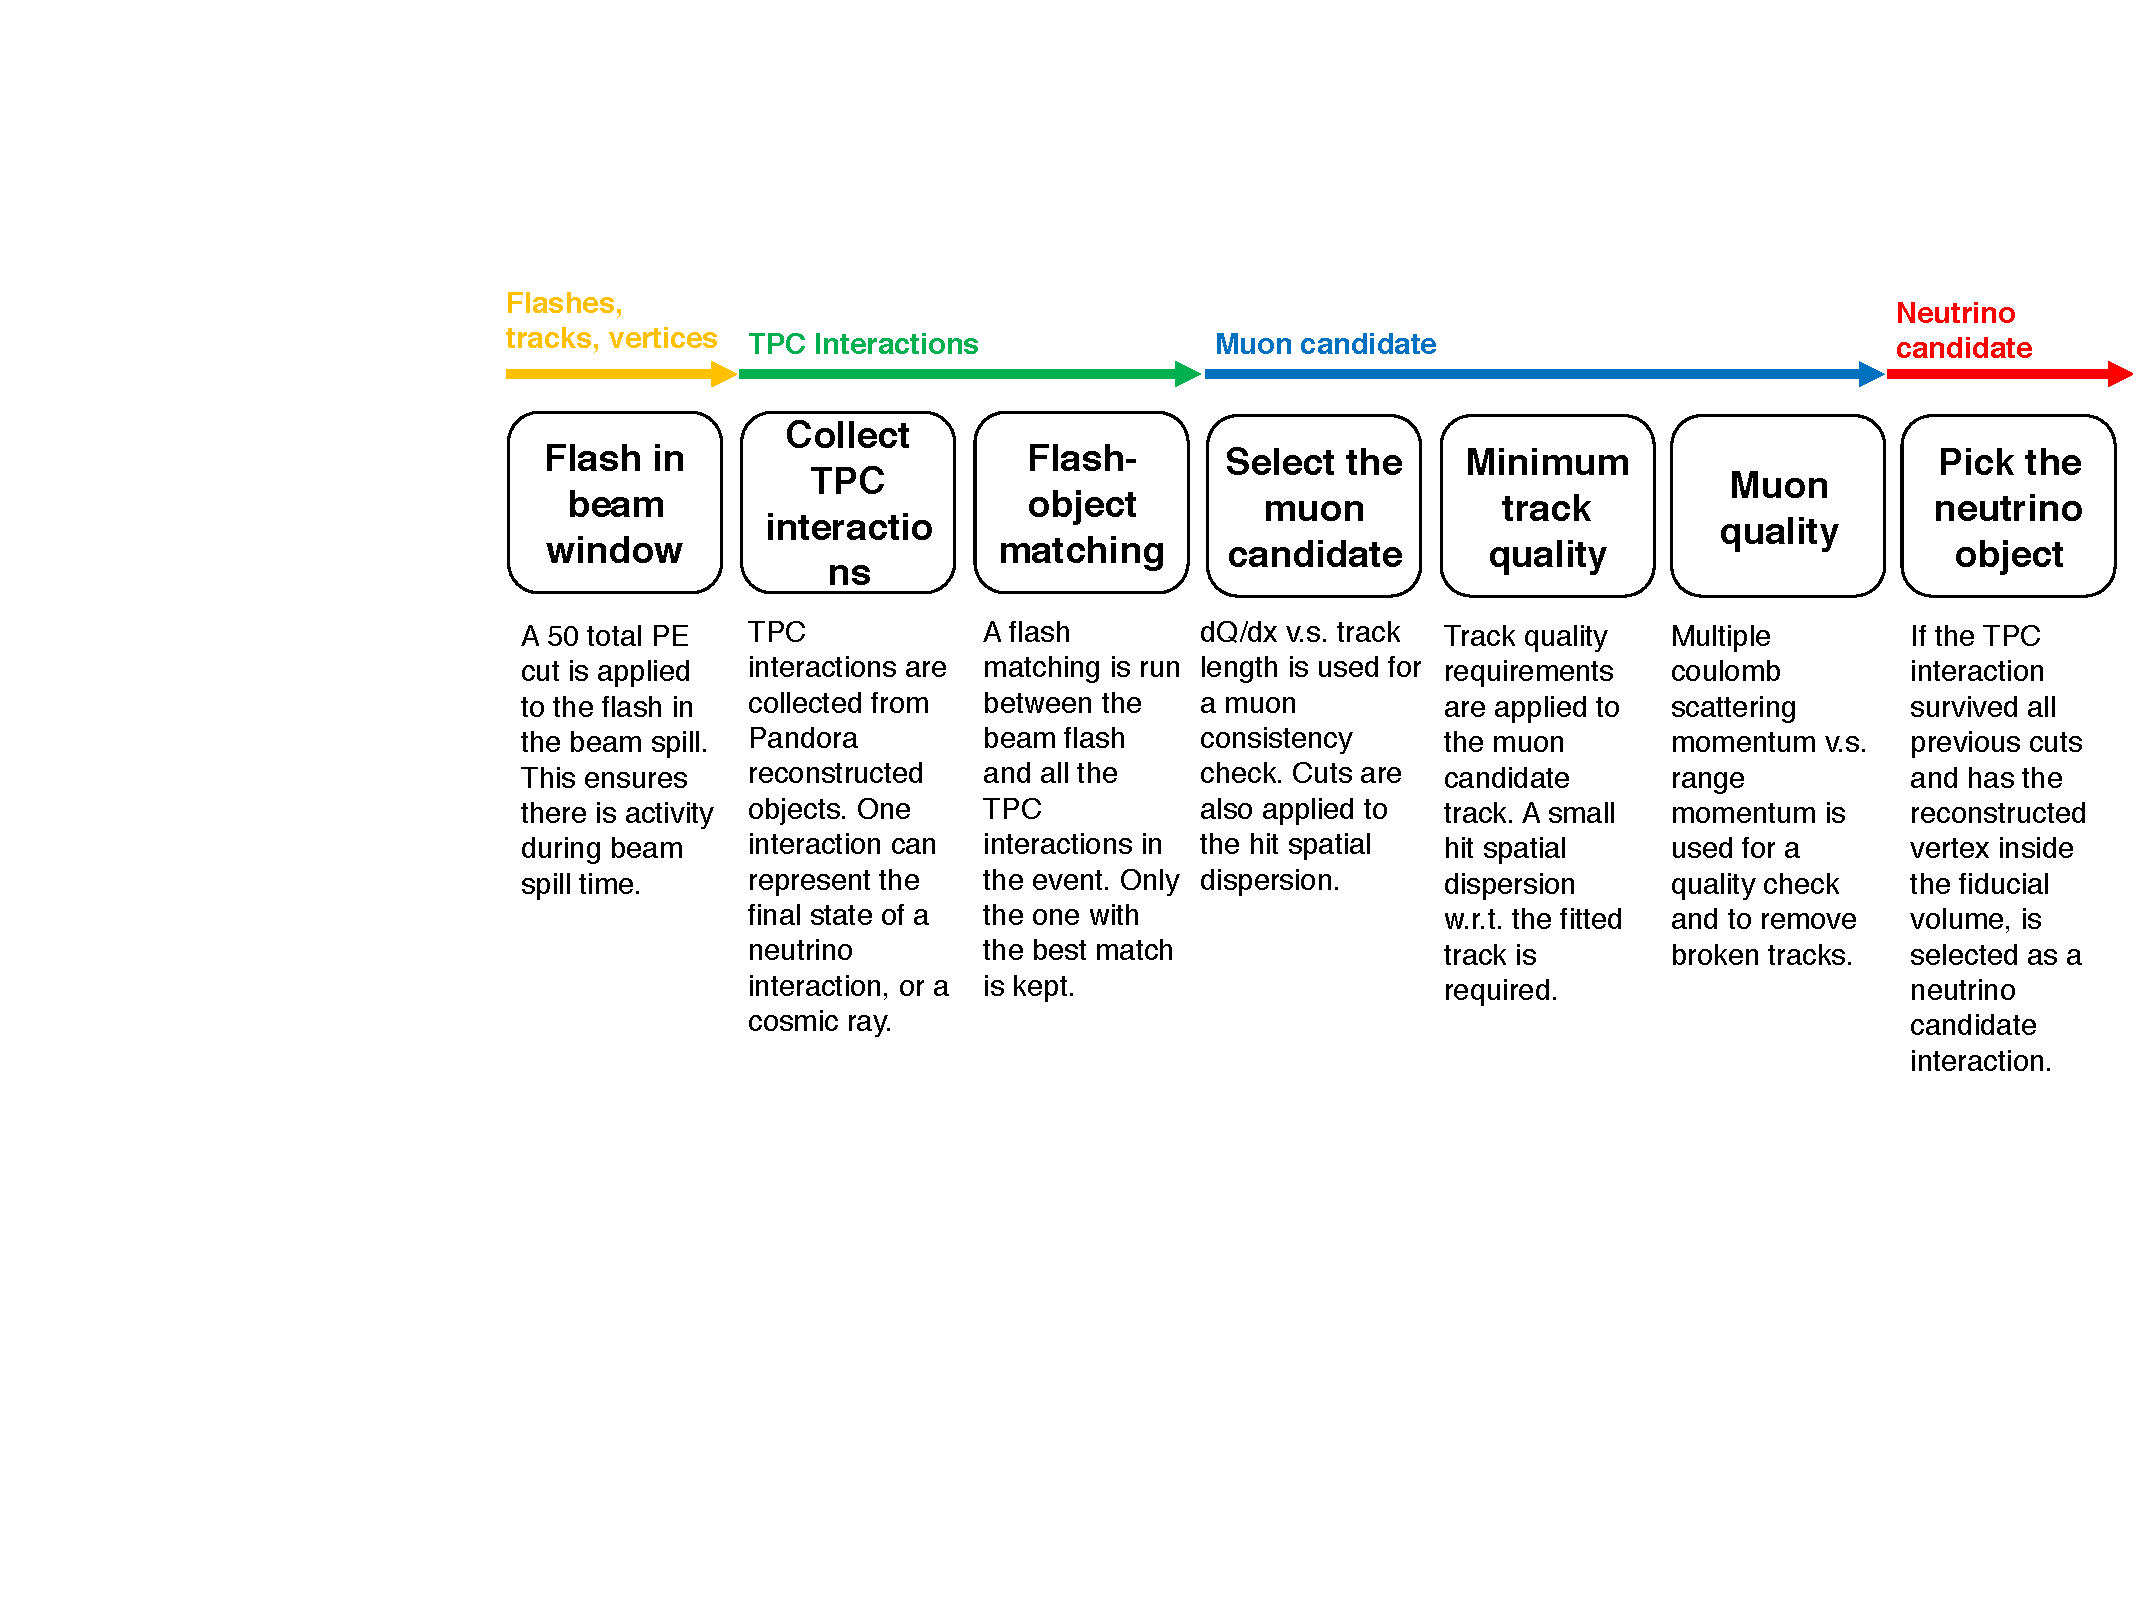
\includegraphics[width=1.0\textwidth]{images/evt_sel_overview}
\caption[Event Selection Overview]{Overview of the event selection used in this analysis.}
\label{fig:evt_sel_overview}
\end{figure}

\section{Beam Spill Flash}
\label{sec:beam_spill}

The first step in the event selection is to remove events where no optical activities are detected in time with the neutrino beam spill. 
One reconstructed flash with more than 50 \acrshort{pe} is required in the beam spill time window. The beam spill duration is 1.6 $\mu$s, and is extended to 1.8 $\mu$s to account for the beam timing jitter, which changes the start and end of the beam window by 0.1 $\mu$s on an event by event basis.

Figure~\ref{fig:flash_pe_0_10000_mcc8_6} shows the total number of \acrshort{pe}s per flash for flashes in the beam spill window. 
The enlarged plot in Figure~\ref{fig:flash_pe_0_300_mcc8_6} shows that signal events do not produce any flashes below 50 \acrshort{pe}. This is also visible in Figure \ref{fig:flash_pe_2}, where the signal efficiency as a function of cut applied on the total number of \acrshort{pe}s is shown. The efficiency presents a plateau at low \acrshort{pe}s, while drops above $\sim80$~\acrshort{pe}.


\begin{figure}[]
\begin{adjustwidth}{-1cm}{-1cm}
\centering
%\subfloat[][Linear Scale.]
%   {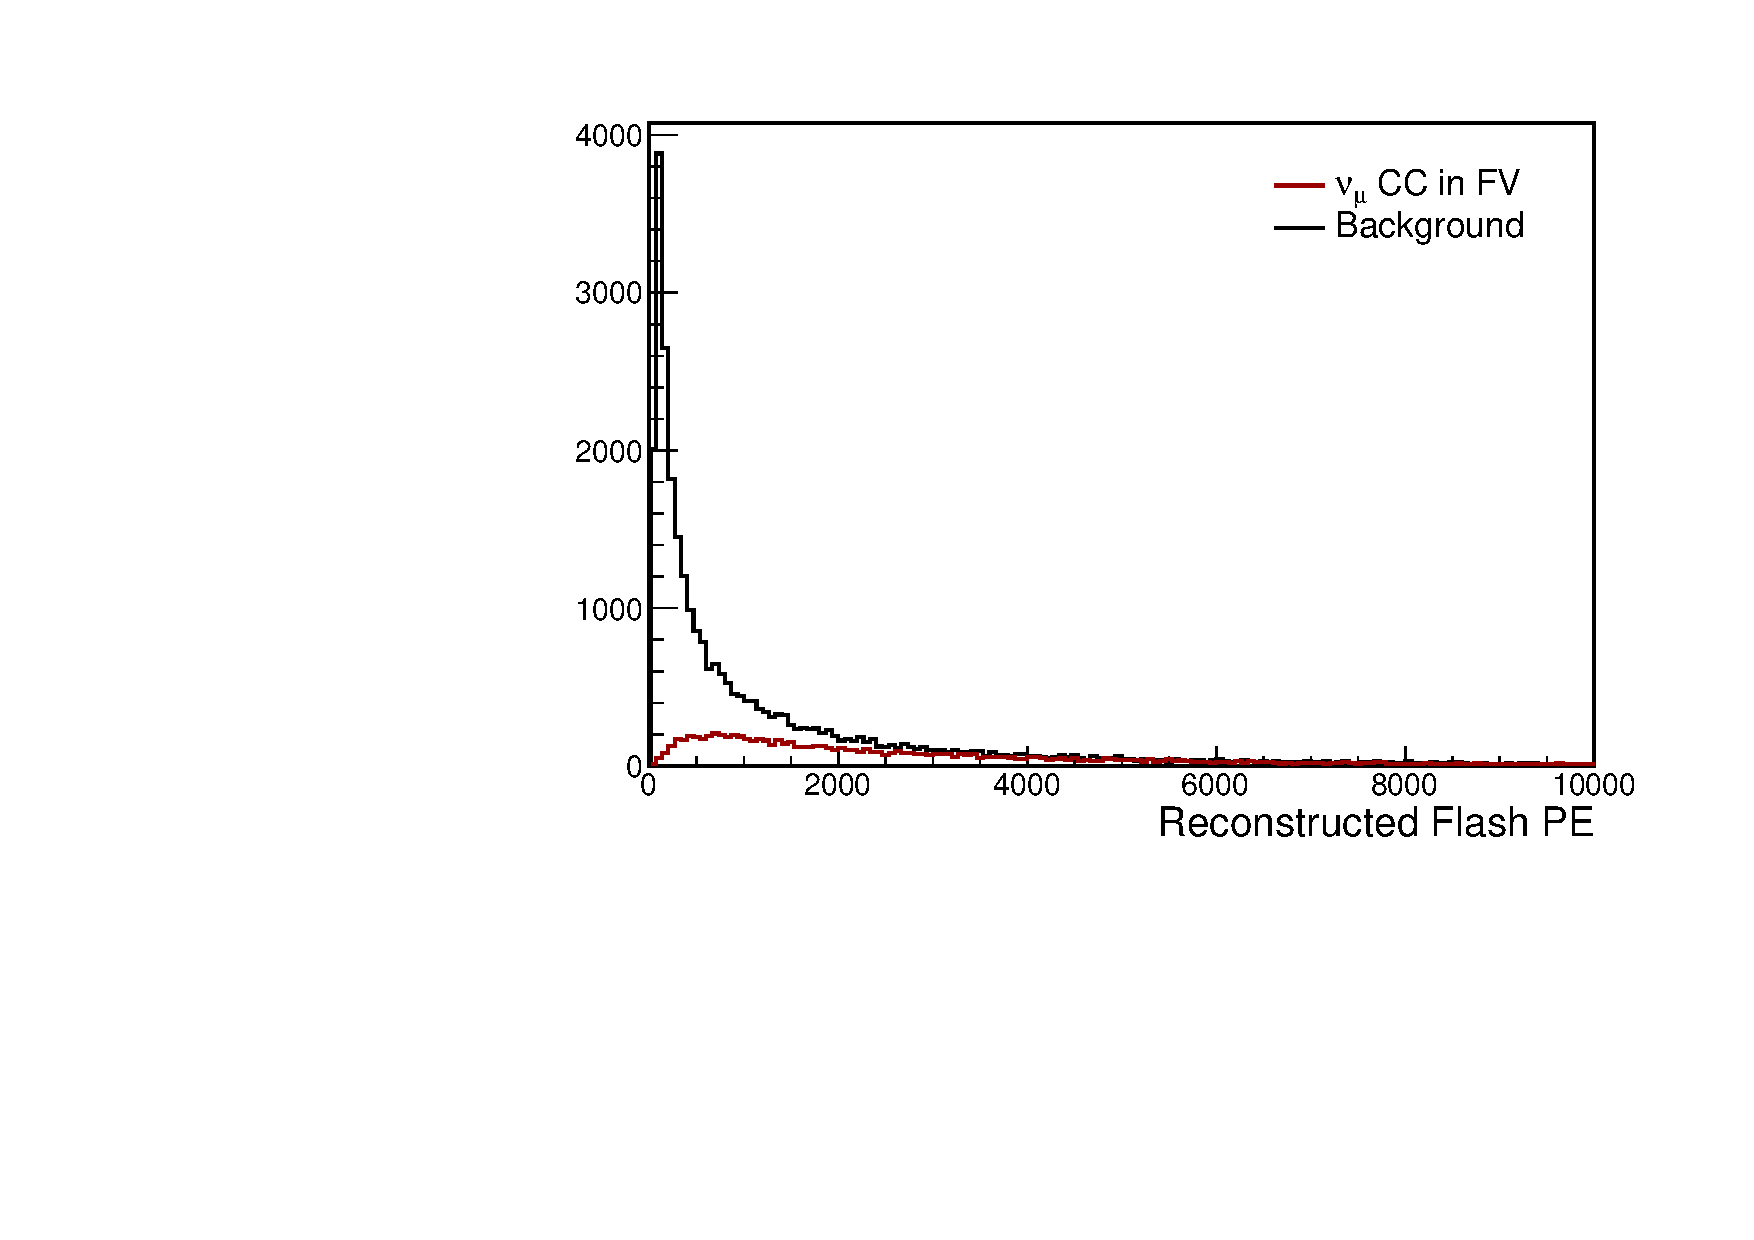
\includegraphics[width=.36\textwidth]{images/flash_pe_0_10000_linear_mcc8_6}
%   \label{fig:flash_pe_0_10000_linear_mcc8_6}} 
\subfloat[][Logarithmic Scale.]
   {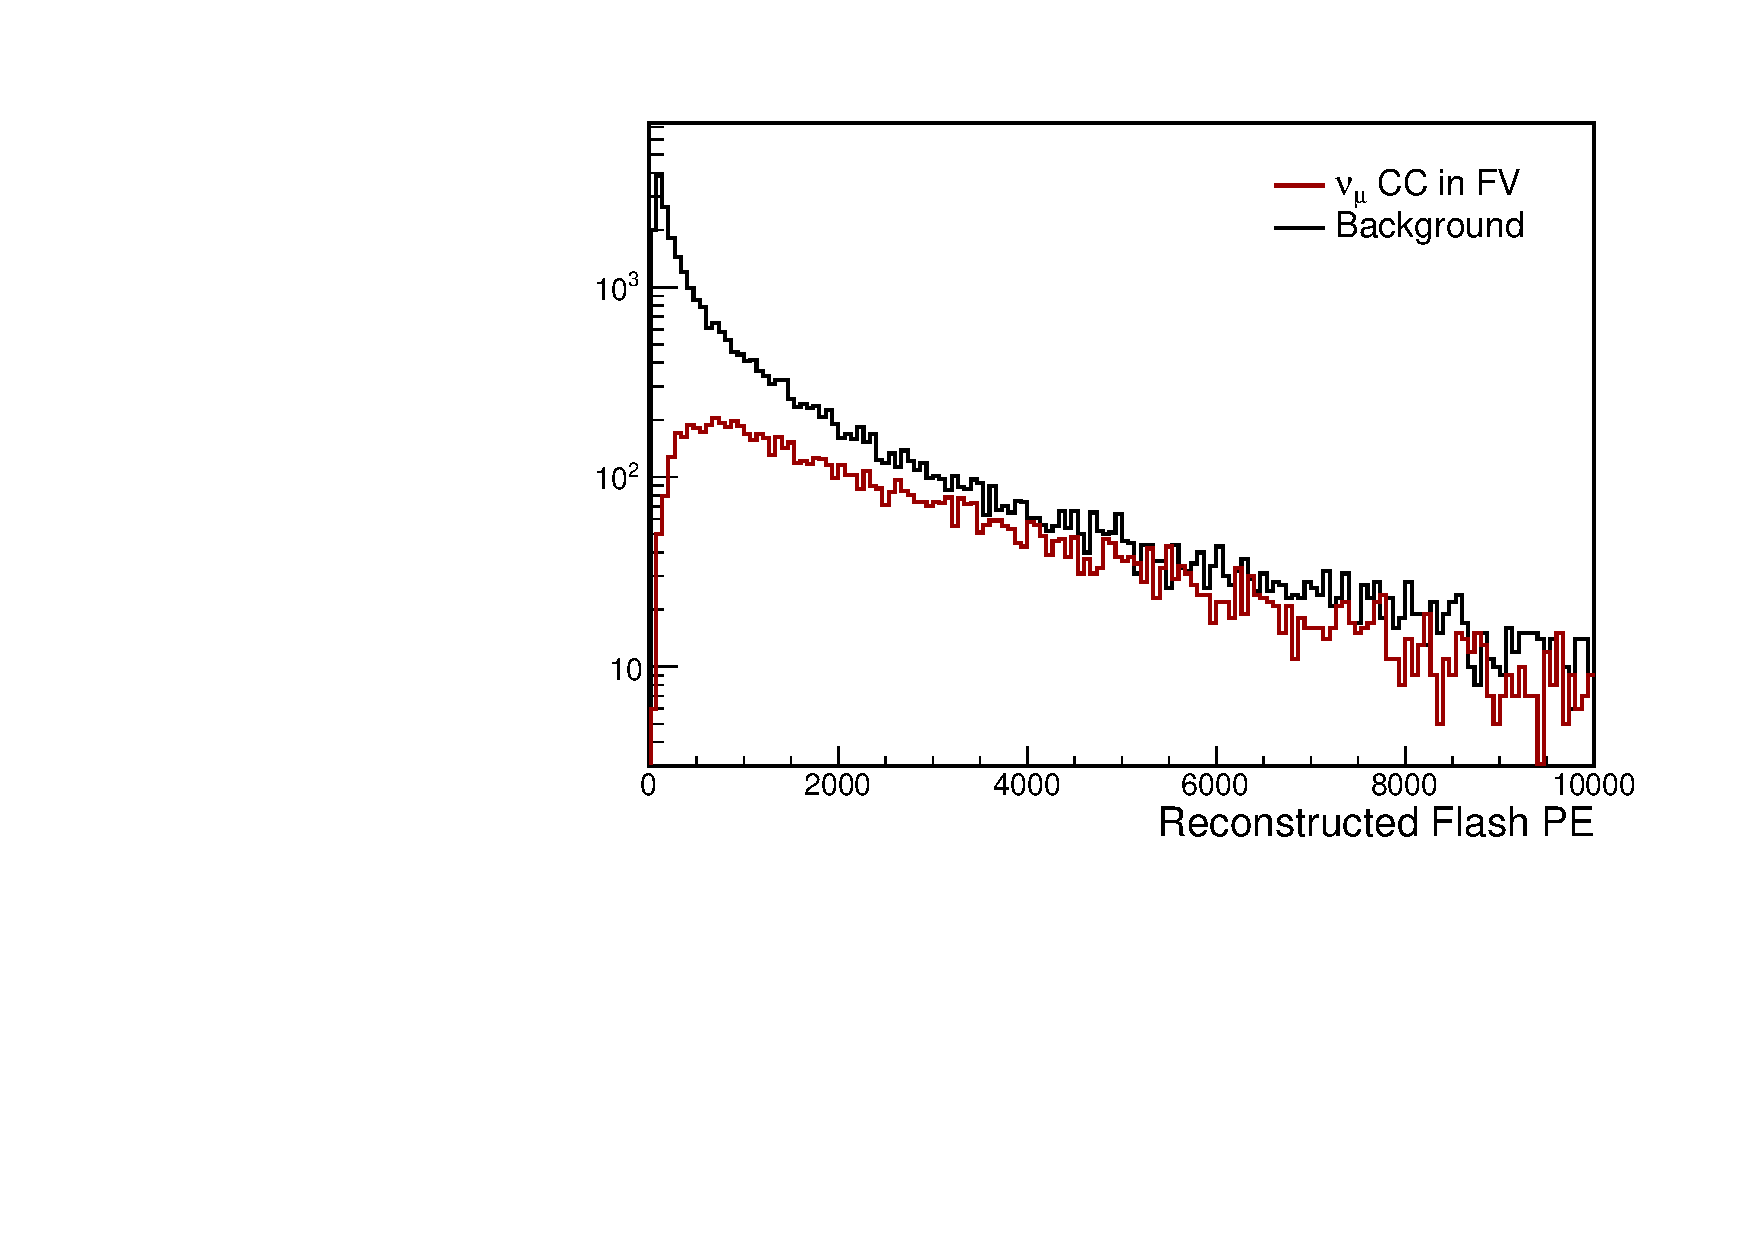
\includegraphics[width=.50\textwidth]{images/flash_pe_0_10000_mcc8_6}
   \label{fig:flash_pe_0_10000_mcc8_6}}
\subfloat[][Enlargement in the low \acrshort{pe} region.]
   {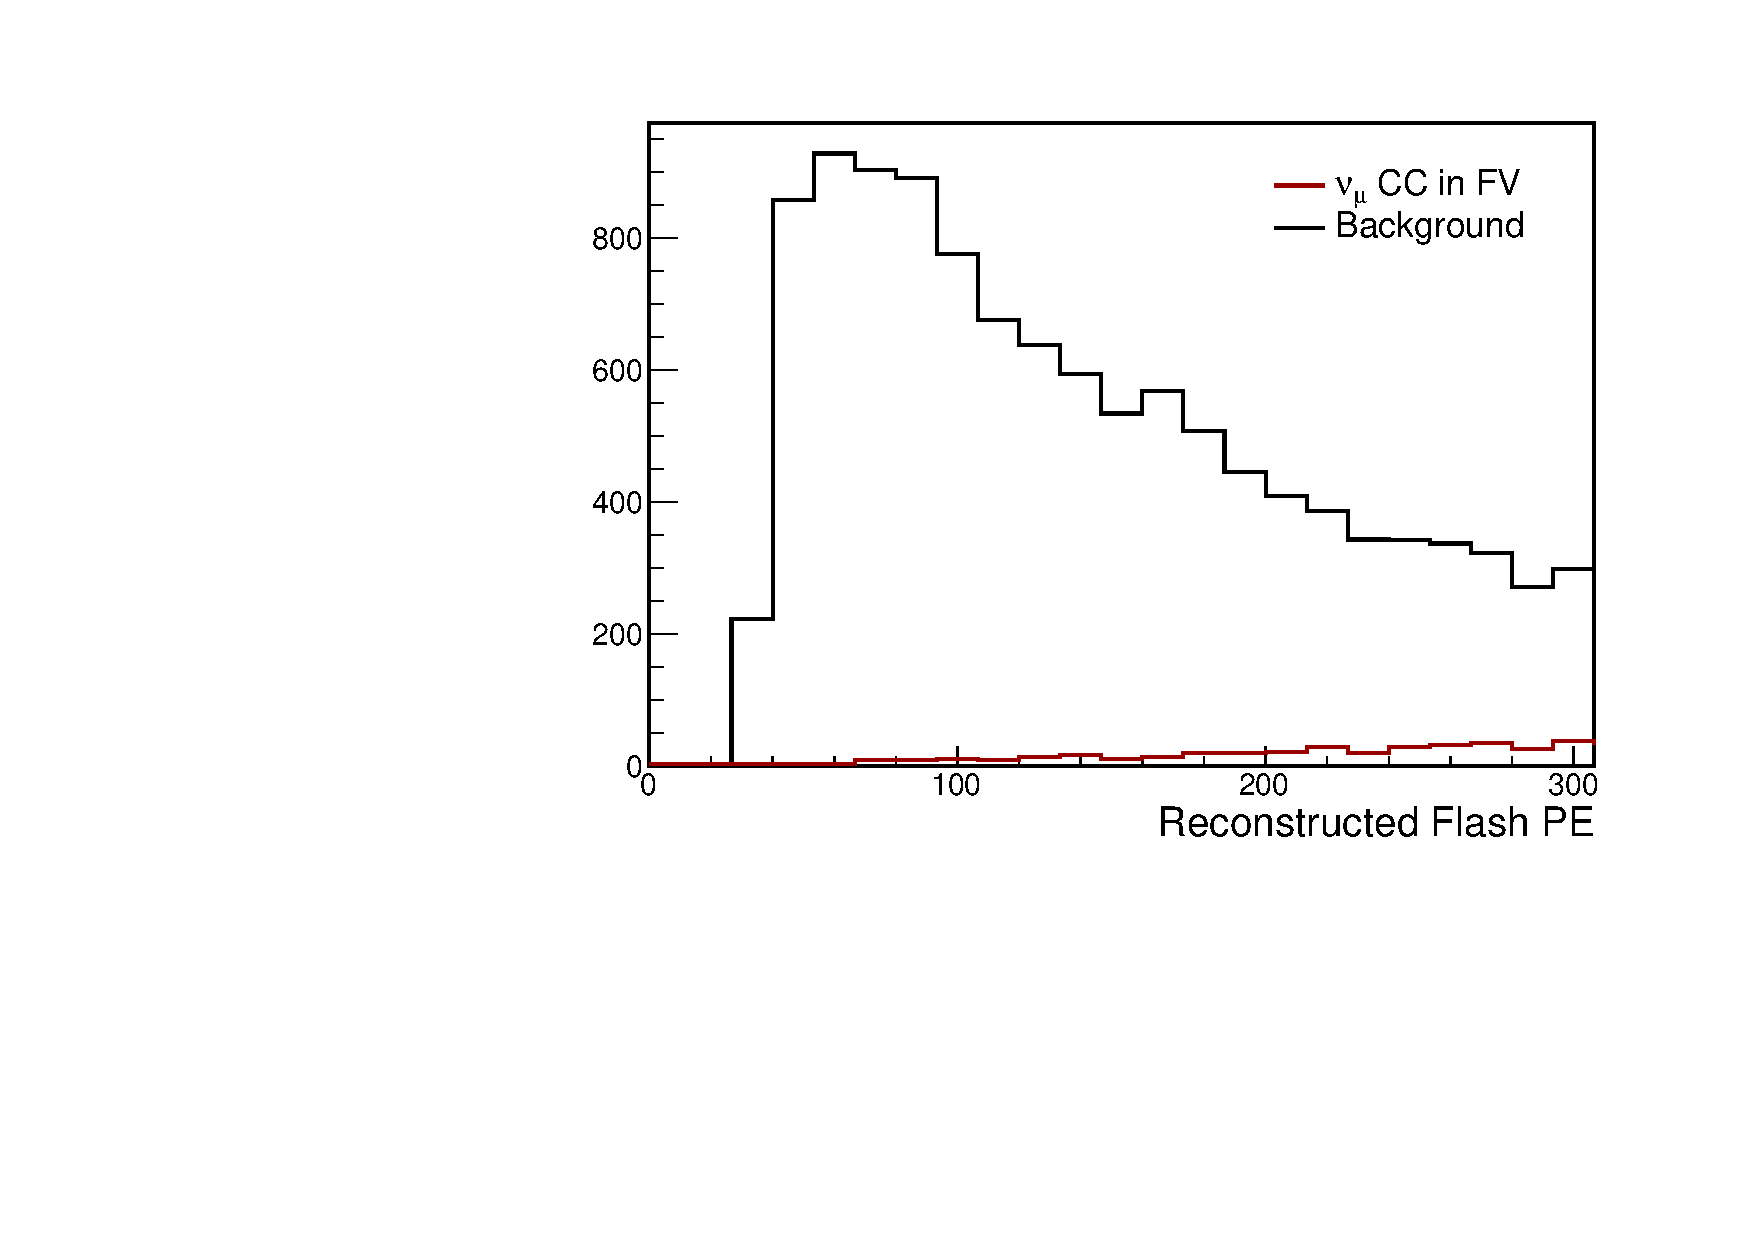
\includegraphics[width=.50\textwidth]{images/flash_pe_0_300_mcc8_6}
   \label{fig:flash_pe_0_300_mcc8_6}} \\ 
\caption[Flash \acrshort{pe} Distribution]{\acrshort{pe} distributions of reconstructed flashes, for flashes in the 1.6 $\mu$s simulated beam spill time window~\protect\subref{fig:flash_pe_0_10000_mcc8_6}. Red is for signal ($\nu_\mu$ \acrshort{cc} events), black for background (all other events). The plot in~\protect\subref{fig:flash_pe_0_300_mcc8_6} is an enlargement in the low \acrshort{pe} region.}
\label{fig:flash_pe}
\end{adjustwidth}
\end{figure}

\begin{figure}[]
\centering
\subfloat[][]
   {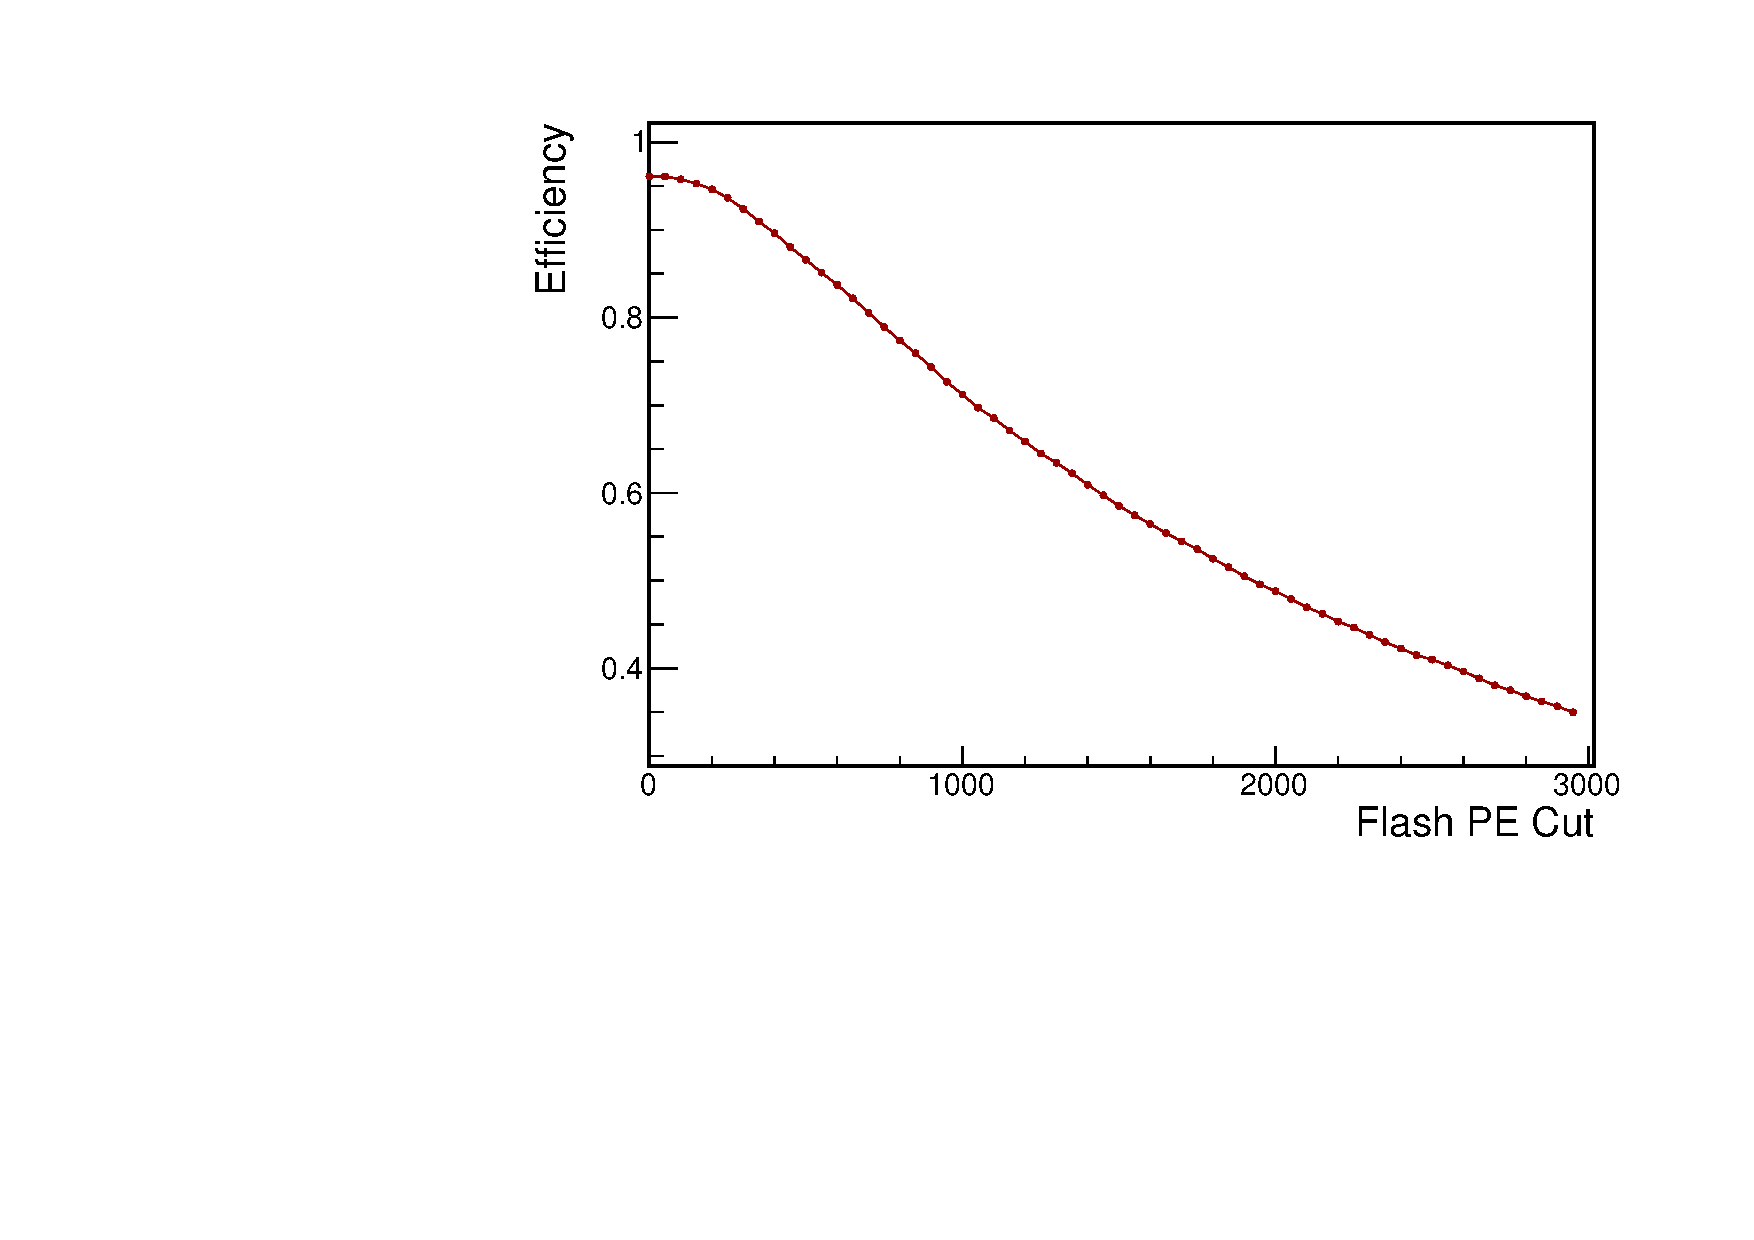
\includegraphics[width=.50\textwidth]{images/eff_pecut_0_3000_mcc8_6}
   \label{fig:eff_pecut_0_3000_mcc8_6}}  
\subfloat[][Enlargement in the low \acrshort{pe} region.]
   {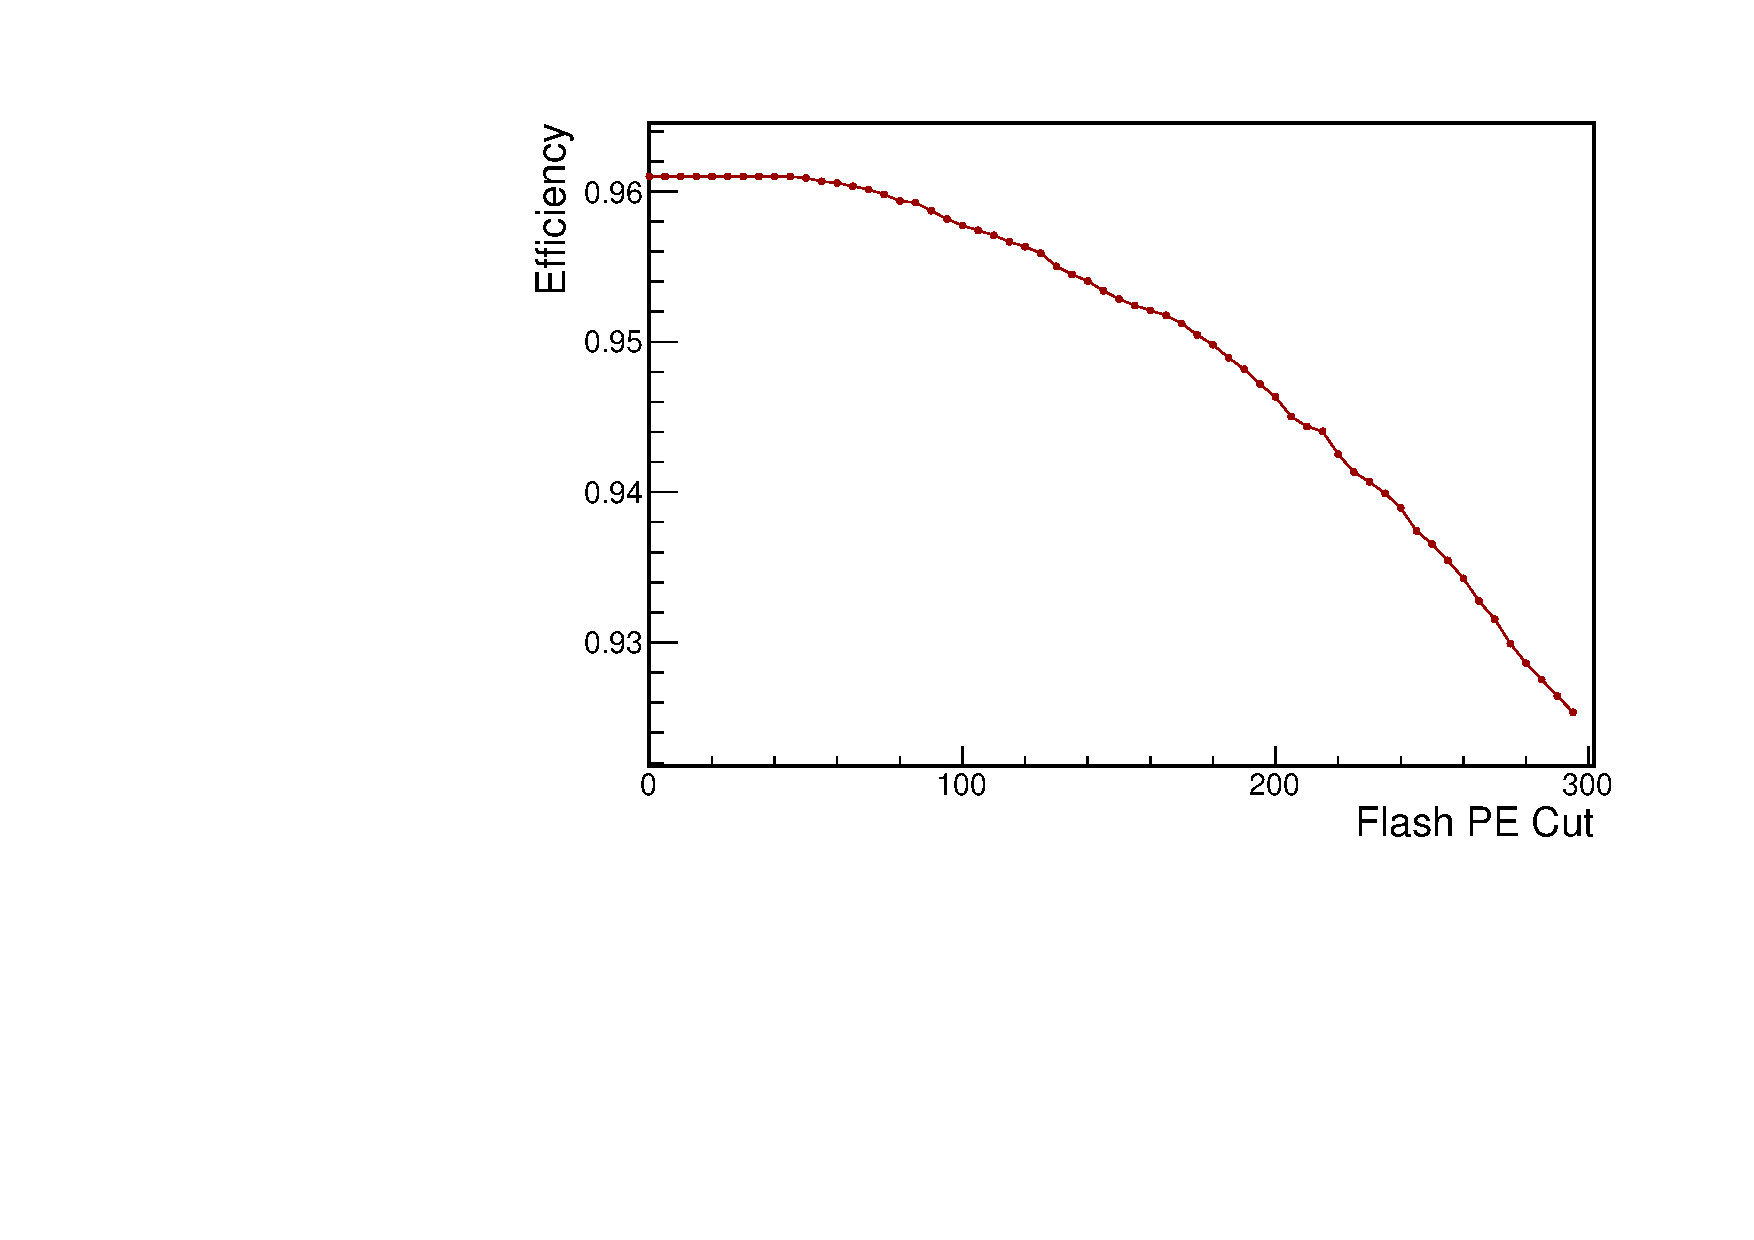
\includegraphics[width=.50\textwidth]{images/eff_pecut_0_300_mcc8_6}
   \label{fig:eff_pecut_0_300_mcc8_6}} \\ 
\caption[Flash \acrshort{pe} Cut Efficiency]{Efficiency of retaining signal events ($\nu_\mu$ \acrshort{cc} events) as a function of the cut applied on the total \acrshort{pe} of the flash in the 1.6 $\mu$s  beam spill~\protect\subref{fig:eff_pecut_0_3000_mcc8_6}. The plot in~\protect\subref{fig:eff_pecut_0_300_mcc8_6} is an enlargement in the low \acrshort{pe} region.}
\label{fig:flash_pe_2}
\end{figure}

Figure~\ref{fig:nu_e_true_flash_sel} shows the effect of the cut at 50 \acrshort{pe} on the true neutrino energy distribution, estimated from simulations. A small number of neutrinos is lost after the cut is applied, while the energy spectrum remains unchanged in shape. For comparison, the energy distribution obtained for neutrinos passing the final selection is also shown.

\begin{figure}[]
\centering
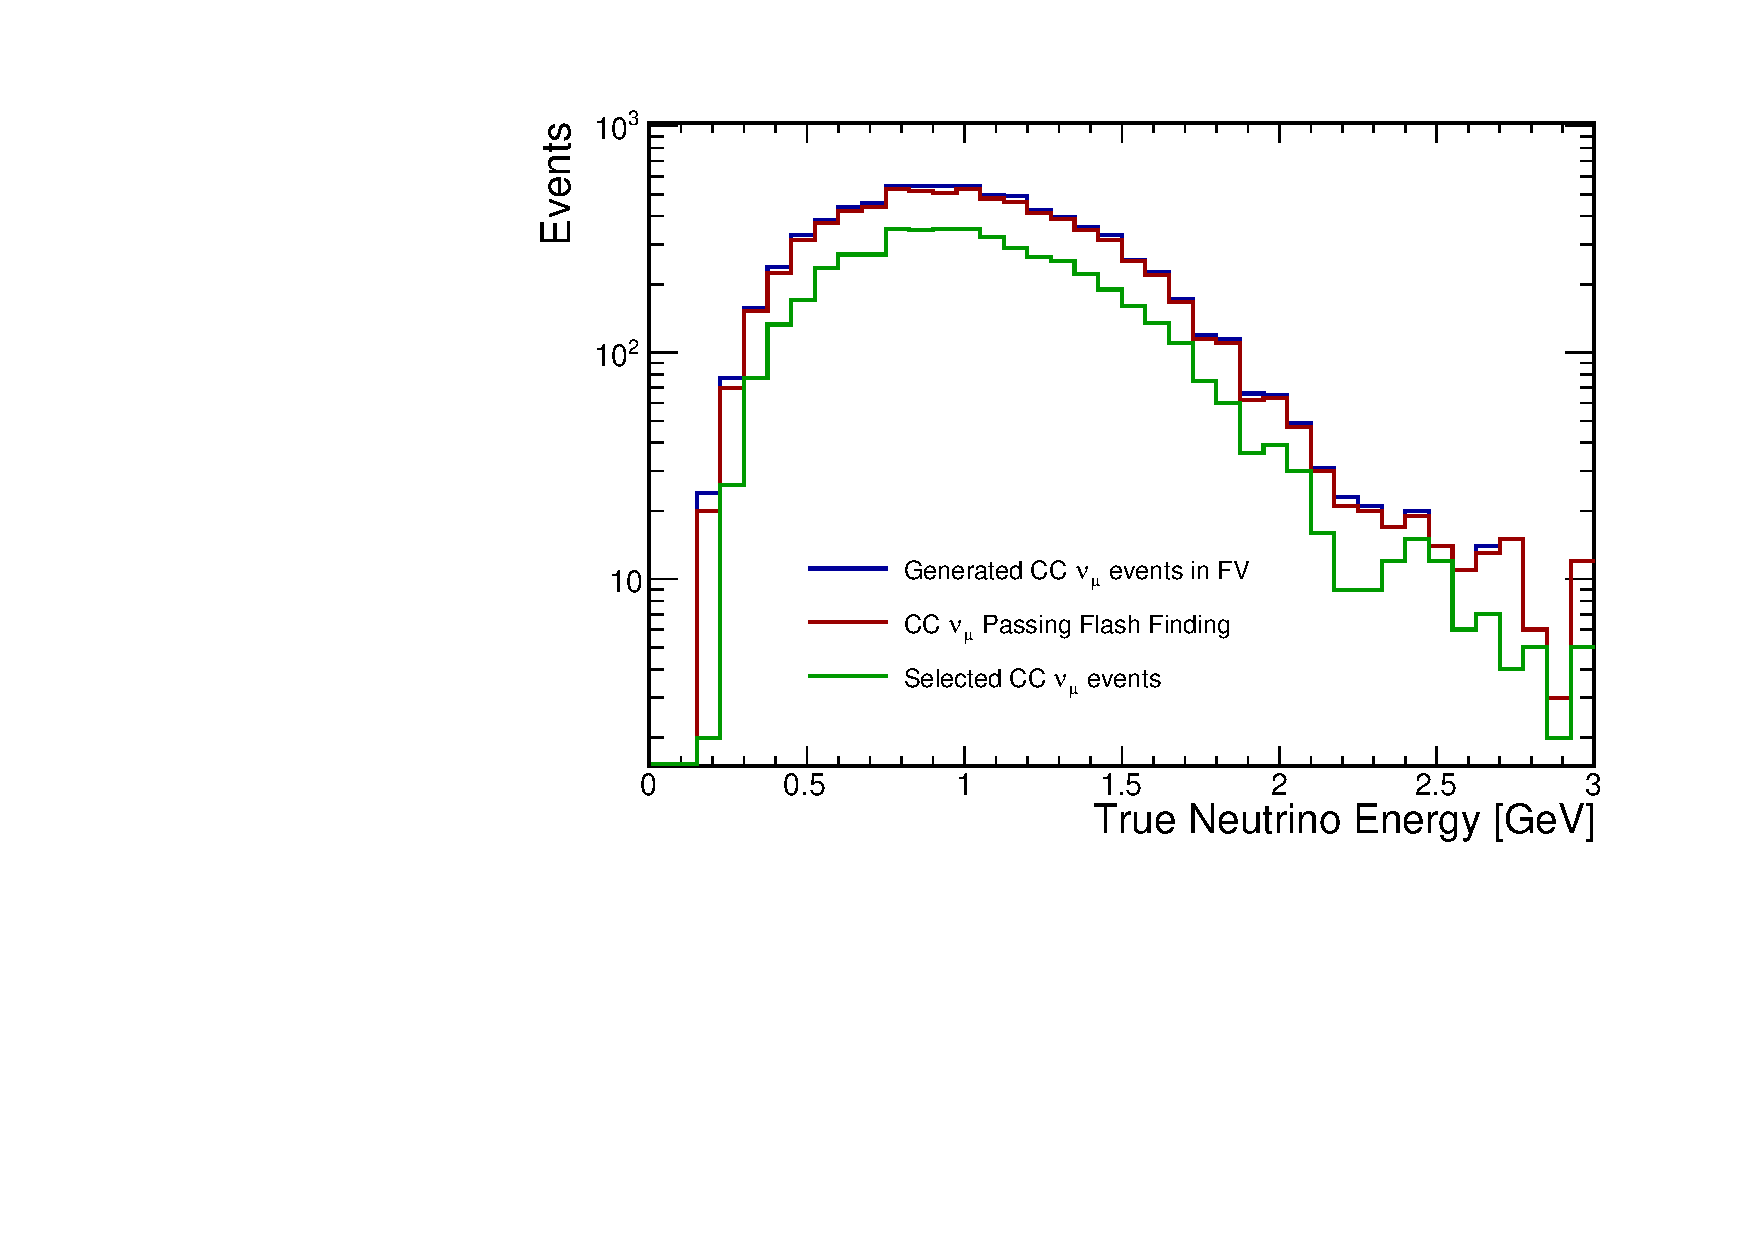
\includegraphics[width=.70\textwidth]{images/nu_e_true_flash_sel}
\caption[True Neutrino Energy Distribution After Flash \acrshort{pe} Cut]{Neutrino energy distributions. The blue histogram shows the generated $\nu_\mu$ \acrshort{cc} events, while the red one shows it immediately after the 50 \acrshort{pe} cut applied on the beam spill selected flash. For comparison, the green histogram shows the distribution of the final selected signal events.}
\label{fig:nu_e_true_flash_sel}
\end{figure}



\section{Additional Flash-Matching Cuts}
\label{sec:selection_fm}

\begin{figure}[]
\centering
\subfloat[][]
   {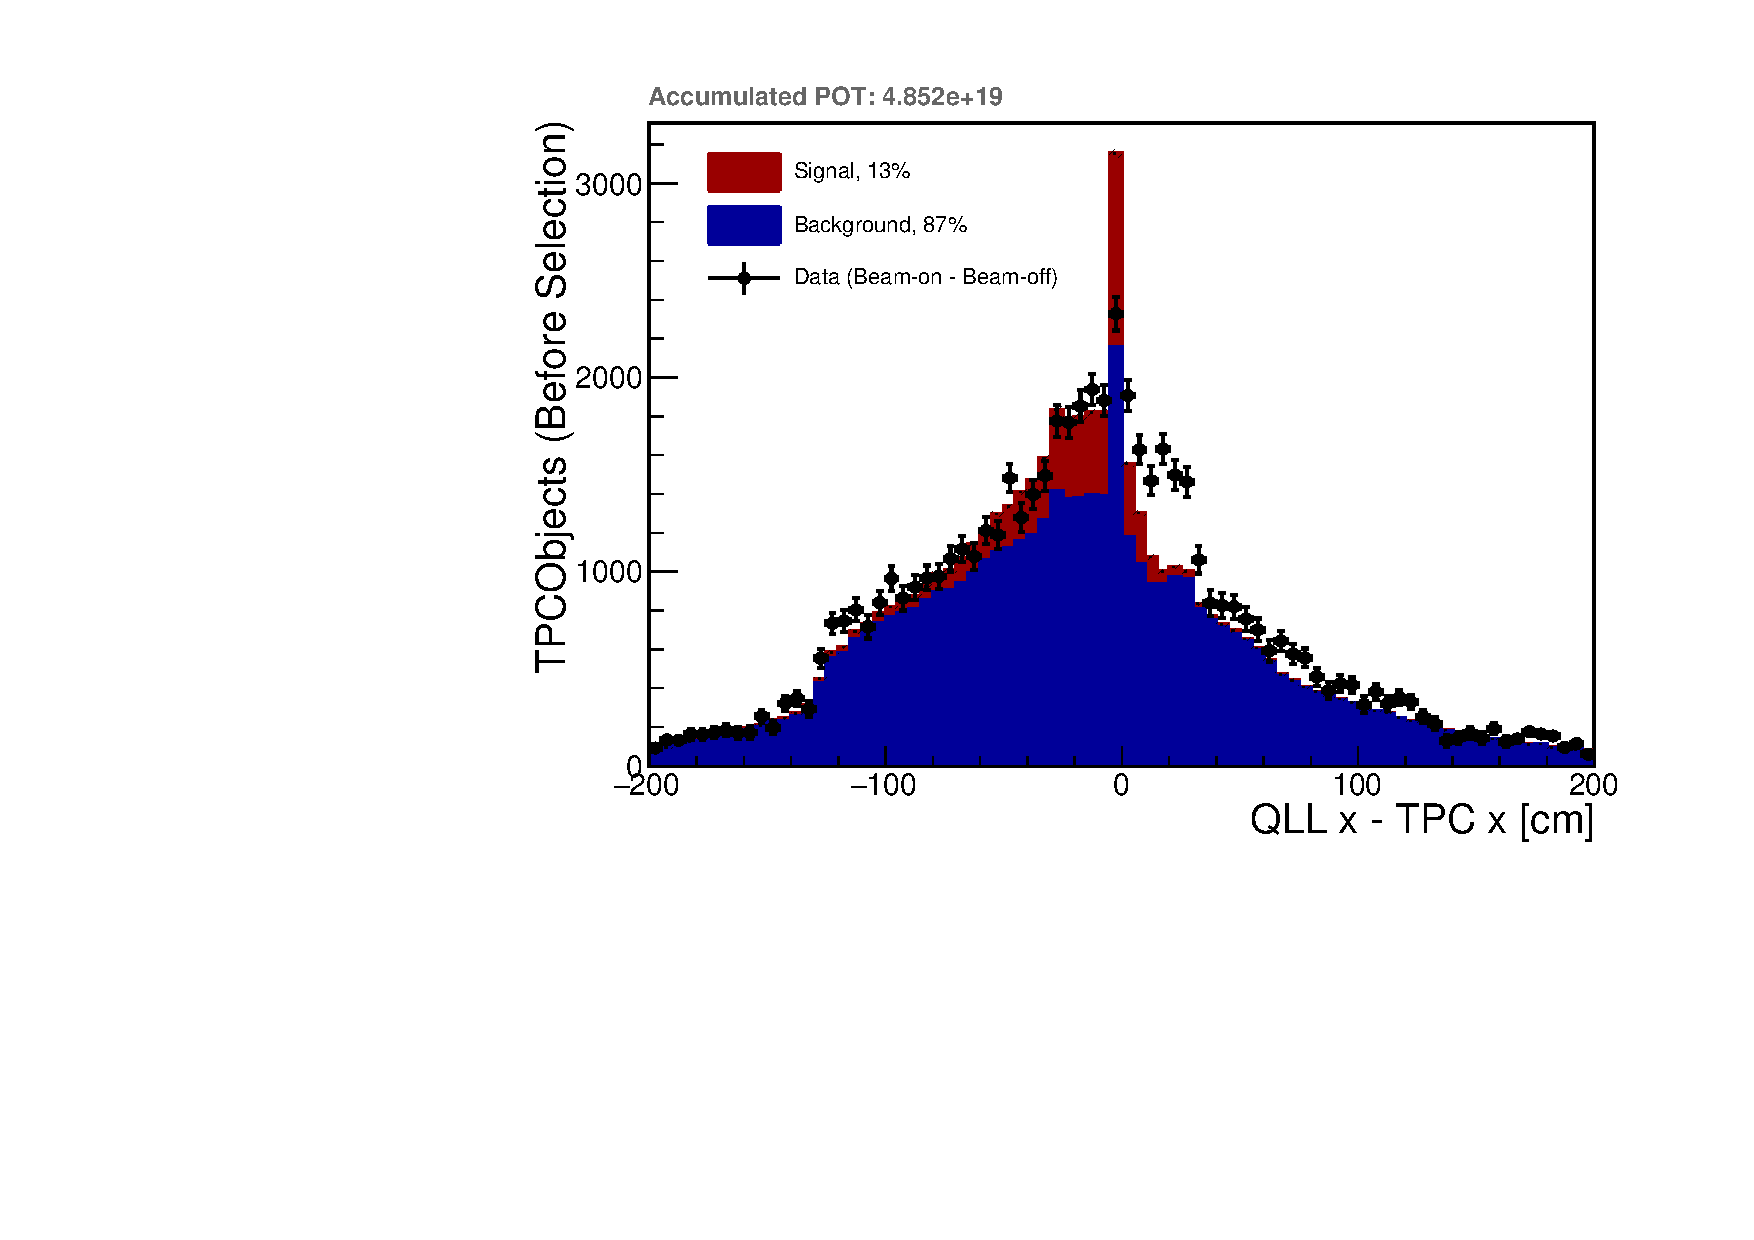
\includegraphics[width=.50\textwidth]{images/fm_deltax_beforesel}
   \label{fig:fm_deltax_beforesel}}
\subfloat[][]
   {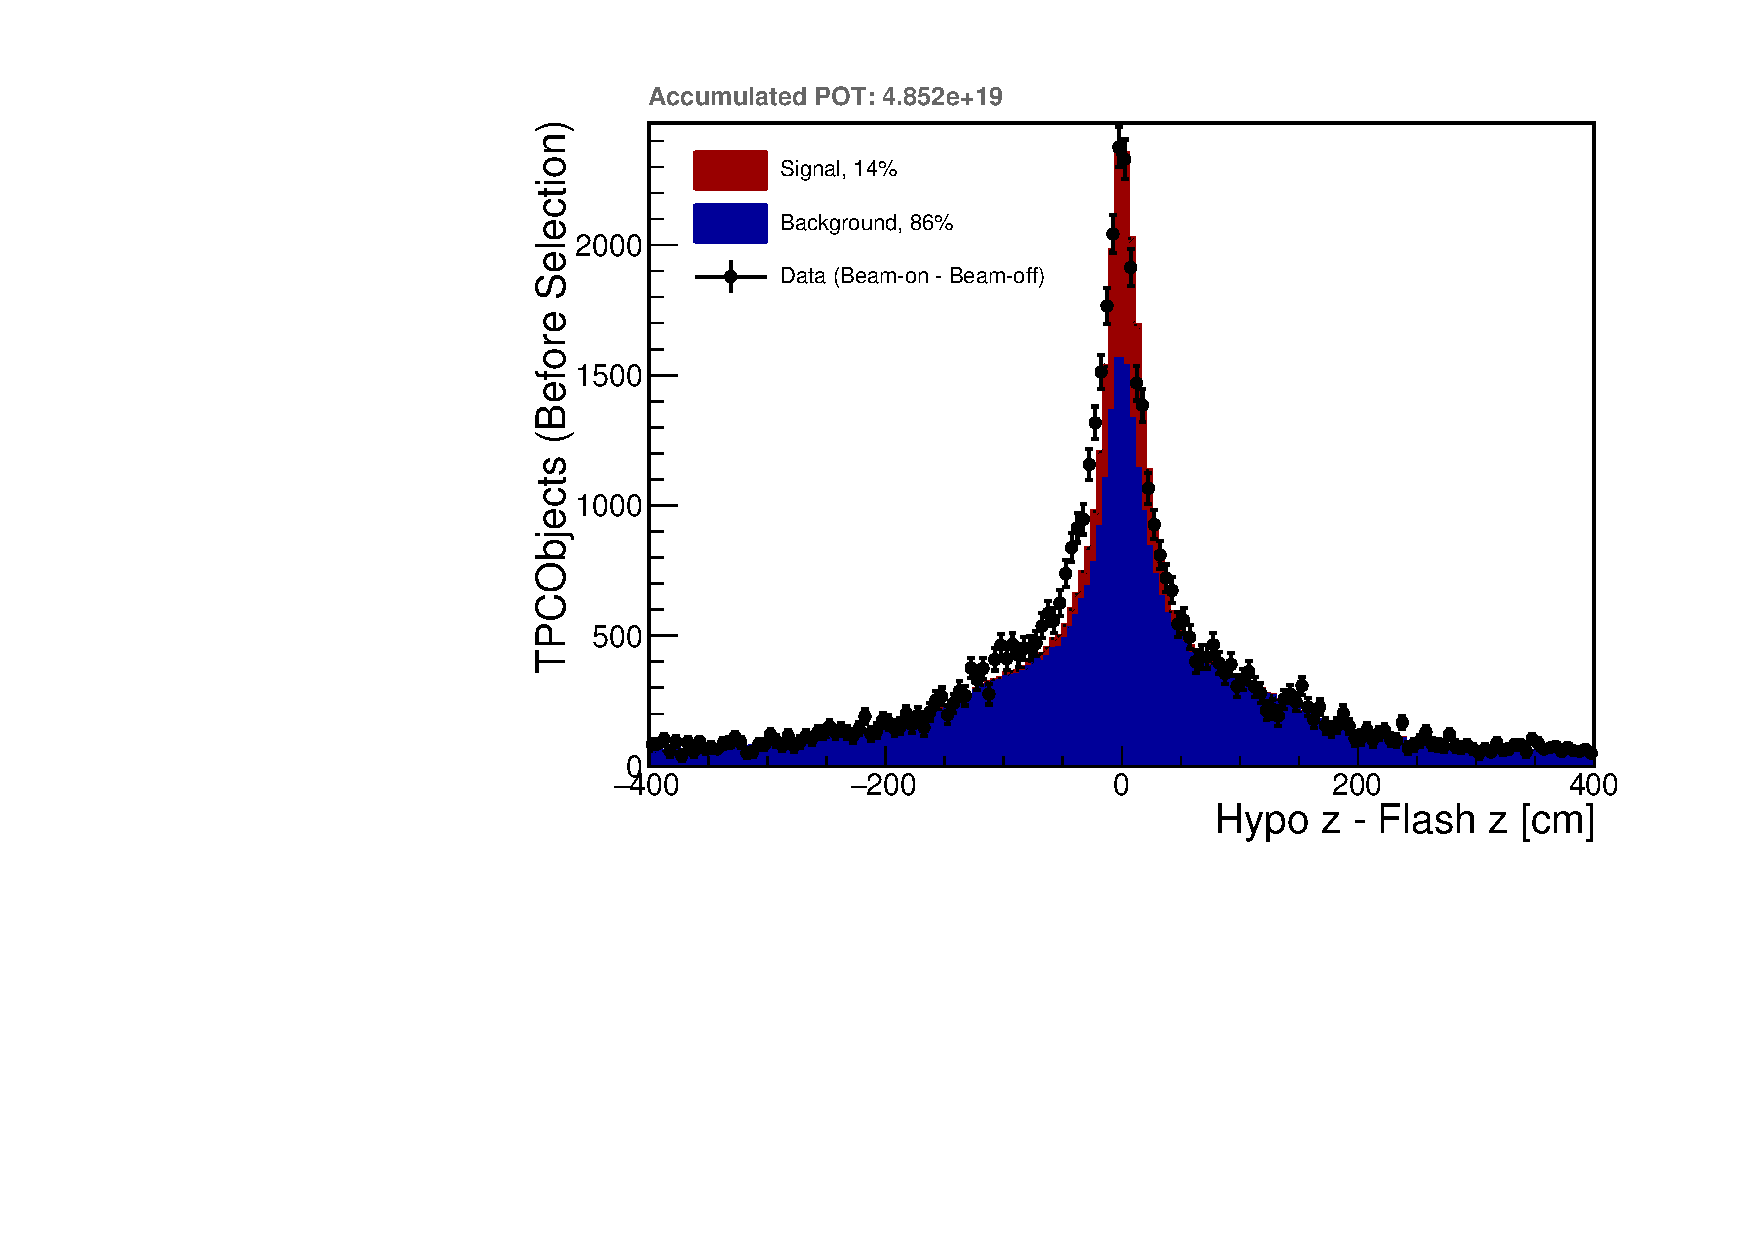
\includegraphics[width=.50\textwidth]{images/fm_deltaz_beforesel}
   \label{fig:fm_deltaz_beforesel}} \\ 
\caption[Flash Matching $\Delta x$ and $\Delta z$]{The left figure shows the difference between the predicted $x$ position and the $x$ position estimated via the flash time. The right plot shows the difference between the $z$ position of the hypothesis flash and the $z$ position of the reconstructed flash. The beam-off data has been subtracted from the beam-on data to make this plot. The red distributions shows simulated signal events ($\nu_\mu$ \acrshort{cc}), while the blue ones show the background event (all other events).}
\label{fig:fm_delta_beforesel}
\end{figure}

The \acrshort{fm} algorithm, described in the Section~\ref{sec:flashmatch}, is run with the flash selected with the criterion introduced in the previous section. The neutrino candidate with the best \acrshort{fm} score is selected by the algorithm, Two additional cuts are applied. The first is applied to the difference between the predicted $x$ position ($QLLx$) of the candidate interaction reconstructed in the \acrshort{tpc} and the $x$ position estimated via the flash time ($TPCx$). The second is applied to the difference between the $z$ position of the hypothesis flash and the $z$ position of the reconstructed flash. The flash $z$ position is calculated according to Equation~\eqref{eq:flash_z}. The distributions of these quantities before the cut is applied are shown in Figure~\ref{fig:fm_delta_beforesel}. Some disagreements between data and simulation are visible in both distributions. In the distribution of the difference in $x$, the data is more smeared than the simulation. To take this into account, a loose cut is applied: events pass this cut if they satisfy  $-100 \leq QLLx - TPCx \leq 50$ cm. In the distribution of the difference in $z$, there is a small offset between data and simulation, this is taken into account with a loose cut such that events with $-75 \leq Z_\text{hypo} - Z_\text{meas} \leq 75$ cm are retained.

%At this point in the event selection, the \acrshort{fm} has allowed to selected either one or no candidate per recorded event. The follow 






\section{Muon Candidate Selection}
\label{sec:selection_muon_candidate}

Given a flash-matched interaction in the \acrshort{tpc}, this interaction is assumed to represent a neutrino interaction in the detector. 
%No selection of \acrshort{cc} over \acrshort{nc} events has been made, yet. 
In order to select \acrshort{cc} over \acrshort{nc} interactions a muon candidate track has to be identified. In fact, a selected interaction usually contains multiple tracks as well as showers, because neutrino interactions can produce multiple particles in the final state. 

Except rare cases where a pion or proton track is the longest among all final state particles, usually the muon candidate track is the longest one. Combining the track length with the particle $\braket{dQ/dx}_\text{trunc}$, as previously described in Section~\ref{sec:tpc_reco}, allows a powerful discrimination between muons and protons.
The distribution of $\braket{dQ/dx}_\text{trunc}$, previously shown in Figure~\ref{fig:dqdx}, shows a good agreement between data and simulation in the proton region (Figure~\ref{fig:dqdx_trunc_calib_protonzoom}), allowing to use this quantity to separate protons from muons.
Figure \ref{fig:dqdx_svm} shows the track length as a function of the track $\braket{dQ/dx}_\text{trunc}$ for the longest track in a flash-matched interaction, and displays cases where such track is a simulated muon or a proton.
% 
\begin{figure}[]
\centering
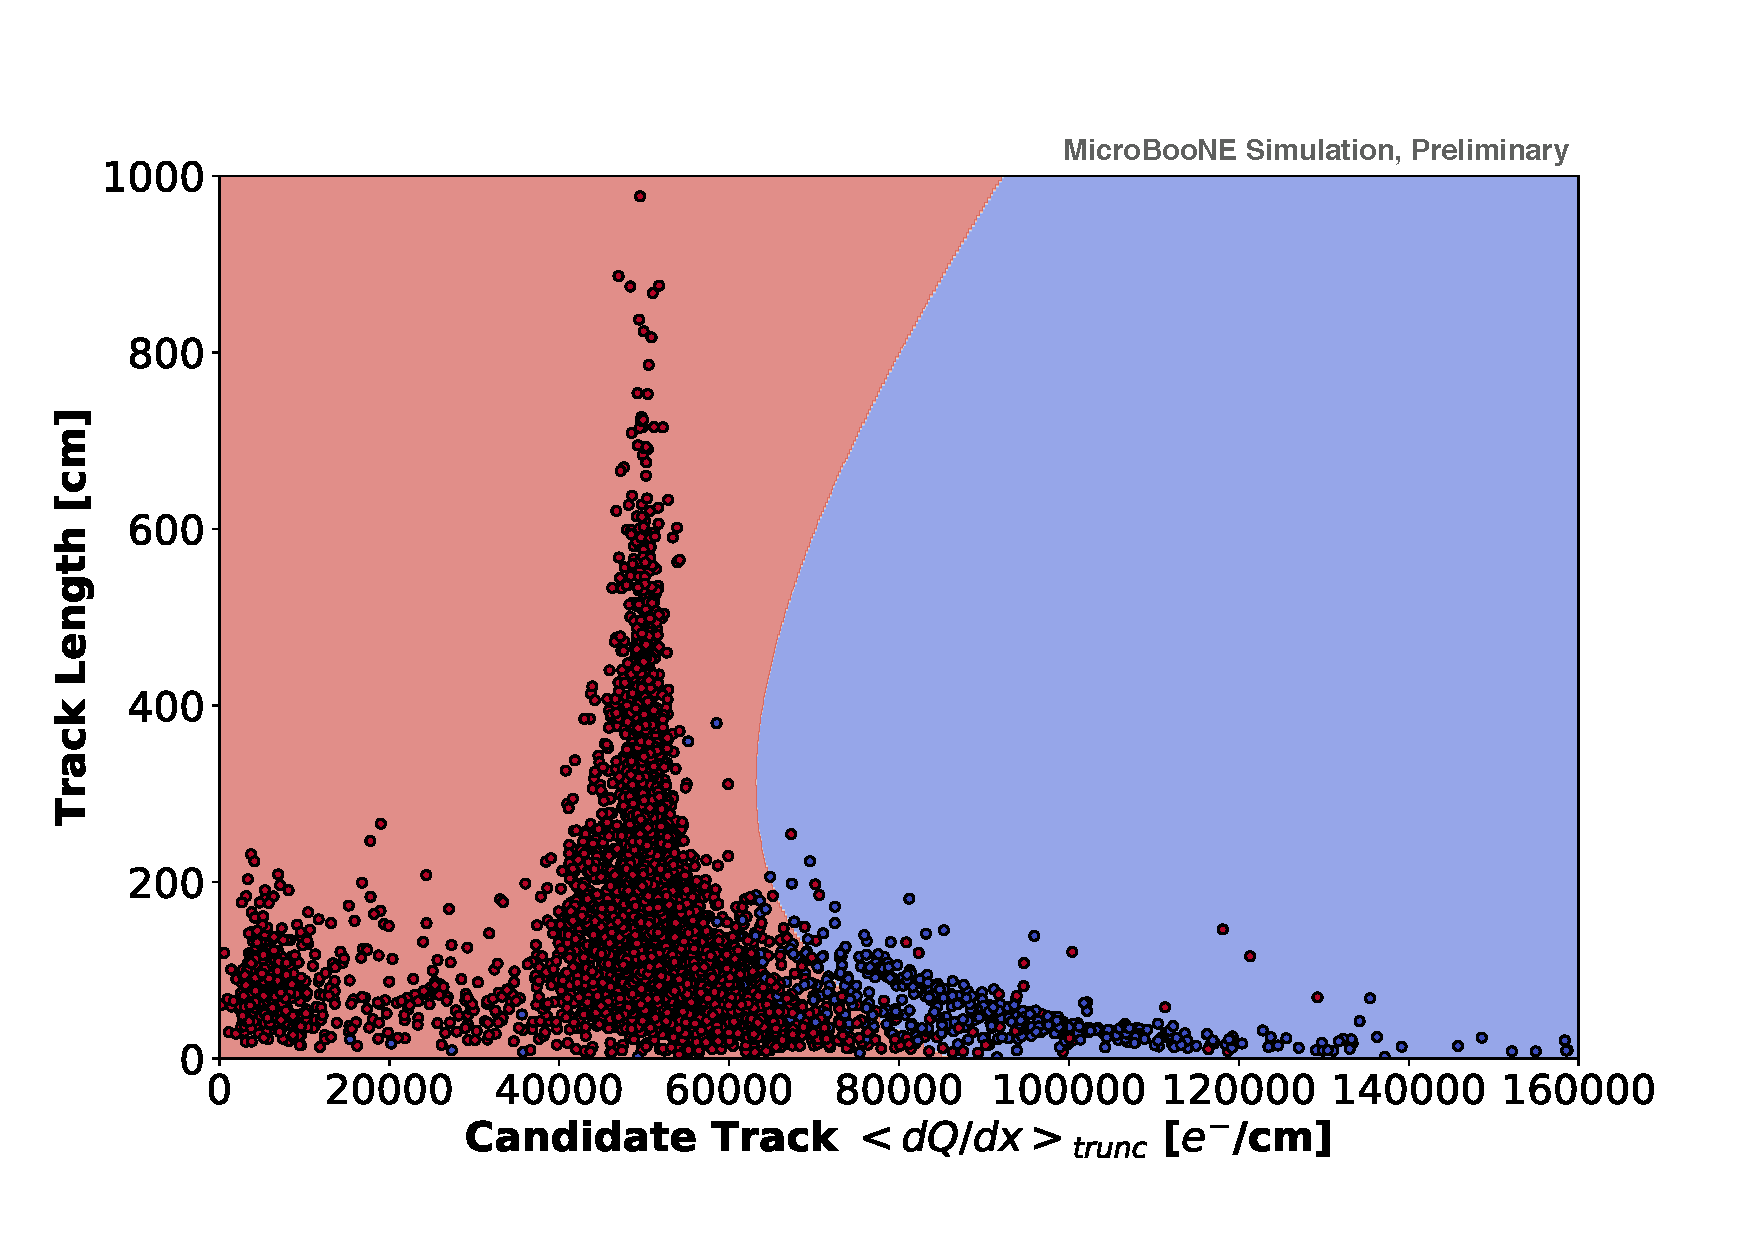
\includegraphics[width=.80\textwidth]{images/dqdx_svm_2}
\caption[Muon/Proton Classification]{Simulated track length as a function of the track $\braket{dQ/dx}_\text{trunc}$ for the longest track in flash-matched interactions. Red dots are simulated muons, blue ones are simulated protons. The light red and blue regions show the output of the \acrshort{svm} classifier. If a track falls in the blue region, it will not be considered as a muon candidate.}
\label{fig:dqdx_svm}
\end{figure}
%
This analysis uses a \acrfull{svm} \cite{svm} algorithm for a muon/proton classification. \acrshort{svm} is a supervised machine learning algorithm which can be used for classification tasks. The algorithm is provided with a training sample, made of vectors $\bm{x}$ that contain the $\braket{dQ/dx}_\text{trunc}$ and the track length $l$, $\bm{x} = (\braket{dQ/dx}_\text{trunc}, l)$, as well as labels for muons and protons. 
Not all the elements of the training sample are used, but only the ones that are near the muon-proton boundary. These are called the ``support vectors'', and are denoted as $\bar{\bm{x}}$.
The goal of the algorithm is to identify a decision boundary that separates the muon and proton populations. The decision boundary is characterised by a decision function $D(\bm{x})$ such that a certain vector $\bm{x}$ is classified as muon if $D(\bm{x}) > 0$ or as proton otherwise.
The decision function $D(\bm{x})$ is found by minimising the Euclidean distance between the decision boundary and the support vectors $\bar{\bm{x}}$.
For this particular application, the decision function is chosen to have the form  
\begin{equation}
D(\bm{x}) =  \sum_{i=1}^{n} \alpha_i K( \bar{\bm{x}}_i, \bm{x}) + \rho,
\end{equation}
where the coefficients $\alpha_i$ and the bias $\rho$ are parameters adjusted by the algorithm during training and $K$ is the so-called Kernel function, here chosen to be
\begin{equation}
K( \bar{\bm{x}}_i, \bm{x}) = \left ( \gamma \, \bar{\bm{x}}_i \cdot \bm{x} + r \right ) ^d,
\end{equation}
with $d = 2$, $\gamma = 0.1$ and $r = 0$. Different parameterisations of the kernel function have been tested, and this one turned out to be giving the best performances in terms of the fraction of events that were classified incorrectly.
The training of the \acrshort{svm} algorithm, aimed to identify the $\alpha_i$ and $\rho$ parameters, was performed on a separate simulated sample. The output of the classifier is shown Figure~\ref{fig:dqdx_svm}. 

To summarise this section, given a flash-matched reconstructed interaction, the candidate muon track is the longest track in such interaction not classified as a proton.








\section{Selected Track Quality}
\label{sec:selection_quality}


Since the goal of this analysis is to provide a cross-section measurement as a function of muon momentum and angle, it is very important to ensure that the muon candidate track and the neutrino vertex are well reconstructed. If the track is reconstructed shorter than its true length, the momentum estimation can be affected. If the vertex is in the wrong position, it may give a wrong value for the muon angle.
Broken tracks, two separate tracks that come from a single vertex, but represent the same particle, are also an issue.
%
\begin{figure}[]
\centering
\subfloat[][]
   {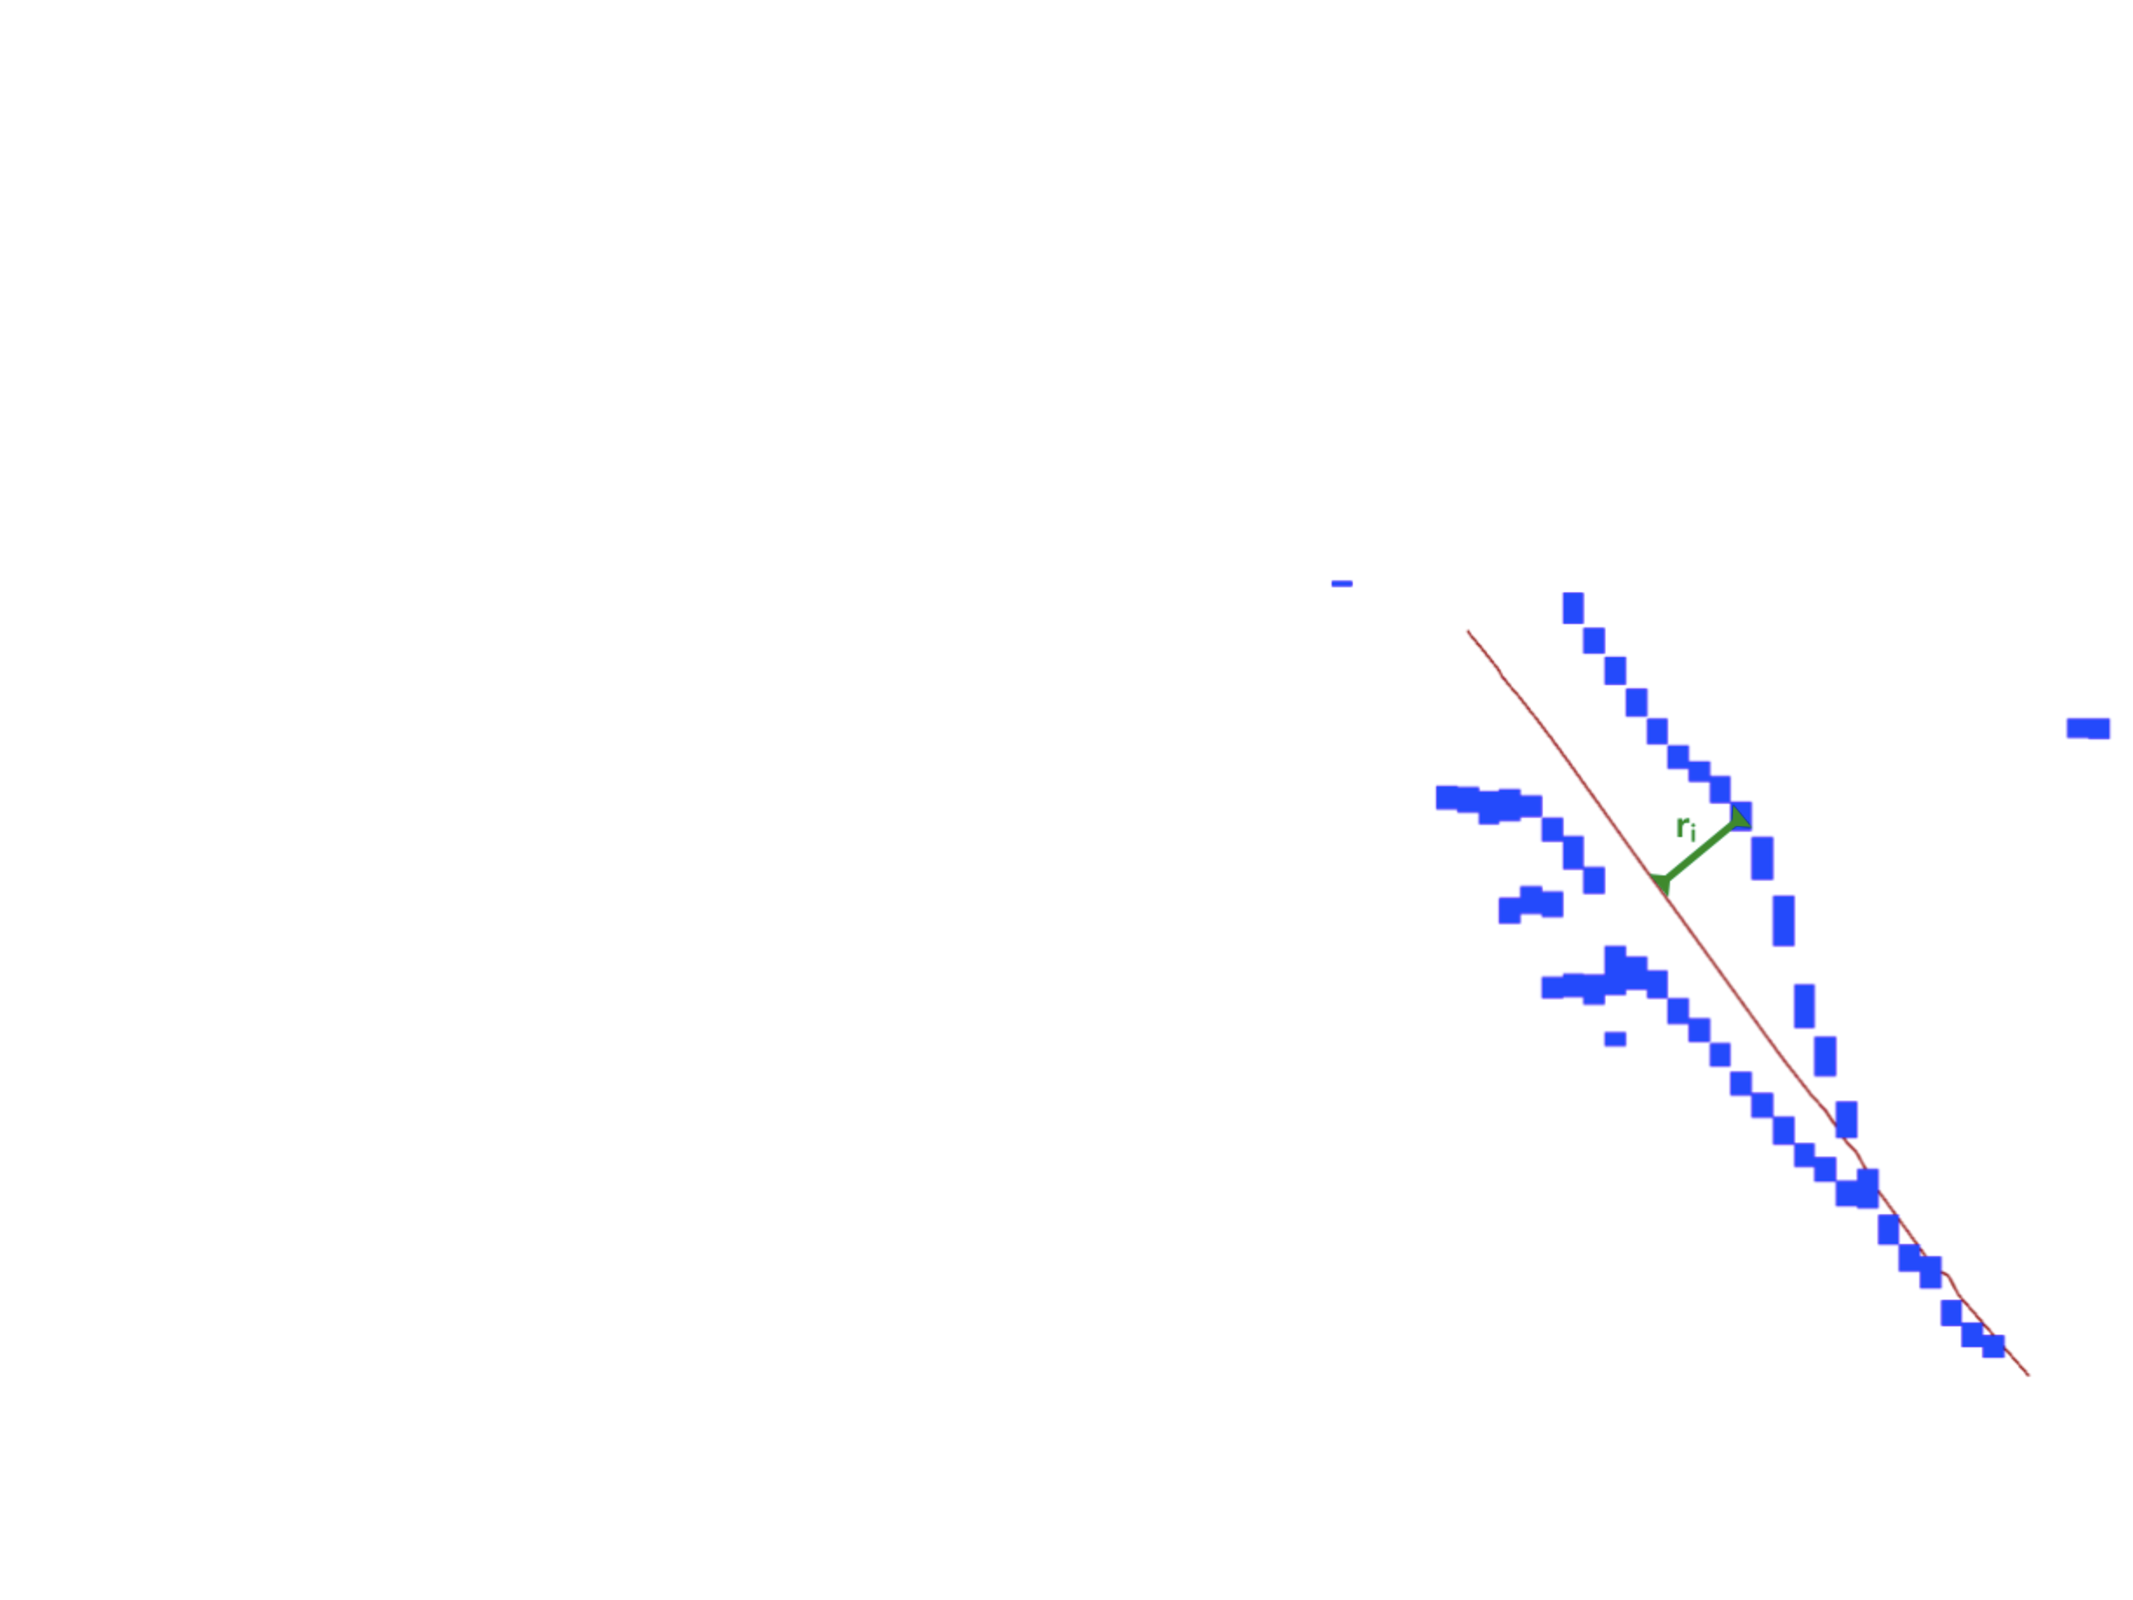
\includegraphics[width=.30\textwidth]{images/figure_hit_residuals}
   \label{fig:figure_hit_residuals}}\quad\quad
\subfloat[][]
   {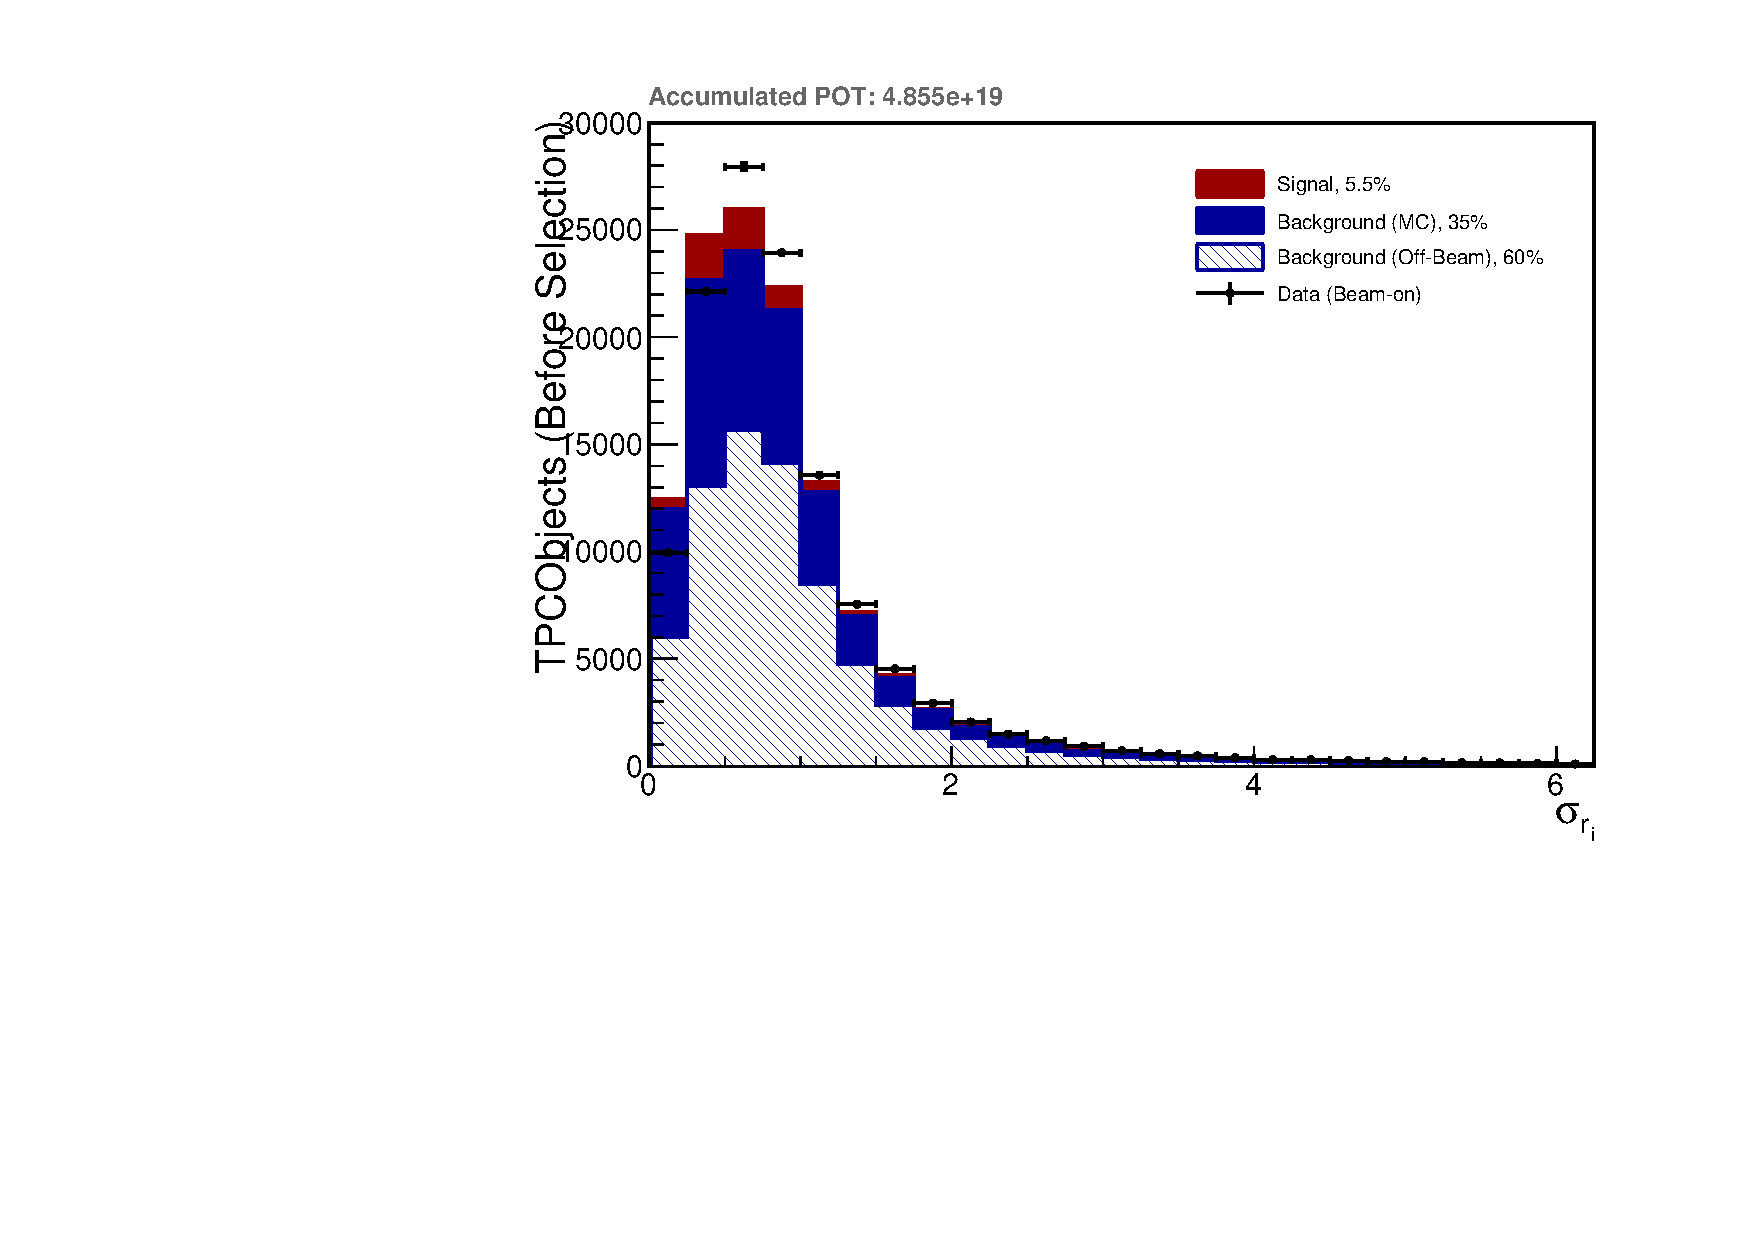
\includegraphics[width=.55\textwidth]{images/aa_residuals_std}
   \label{fig:aa_residuals_std}} \\ 
\caption[Distribution of Hit Residuals]{\protect\subref{fig:figure_hit_residuals}~Illustration of how the hit residuals are calculated, taking the projection of the track on the collection plane, and measuring the distance between the hit and the closest track trajectory point. \protect\subref{fig:aa_residuals_std}~Distribution of the \acrshort{std} of the hit residuals in the collection plane for all flash-matched interactions. Black points are data points. The coloured histograms show the beam-off \acrshort{cr} contribution (hashed), the simulated background (blue) and the simulated $\nu_\mu$ \acrshort{cc} signal events (red).}
\label{fig:aa_trk_quality_residuals}
\end{figure}
%
Another issue arises when electrons or photons, producing electromagnetic showers, are reconstructed as tracks. Electrons and photons should be reconstructed as shower objects as they do not produce a track-like signature in the detector. To remove these mis-reconstructed tracks, the distribution of the hits in the collection plane is studied, to check if the hit dispersion along the track is small. If it is large, then the track is most likely fitting a shower-like object. 
The hit residuals $r_i$ are defined per each hit as the two dimensional distance between the hit and the closest track trajectory point projected onto the collection plane. Figure~\ref{fig:figure_hit_residuals} shows a one-event example, where a track fits a collection of hits from a shower-like particle. For every event, the \acrshort{std} of the residual distribution, $\sigma_{r_i}$, is considered, and it is shown in Figure~\ref{fig:aa_residuals_std} for all events at an intermediate stage in the event selection, after the flash matching has been applied, and after the muon candidate track has been selected. Tracks that populate the high $\sigma_{r_i}$ region have a high hit dispersion with respect to the track trajectory and a cut is applied so that events are selected if they have $\sigma_{r_i} < 2.5$ cm.

The track reconstruction actually takes as input reconstructed three dimensional space points, that are created by matching two dimensional hits from all three wire planes. An additional way to understand if the track is well reconstructed is to look at the number of hits that are associated to space points used for the track fitting. 
If the particle is not track-like, fewer hits will be associated to space points. The ratio between the number of hits associated to space-points and the total number of hits in the cluster allows to identify mis-reconstructed tracks. Only hits in the collection plane are used. Figure \ref{fig:aa_trk_quality_frac_used_hits} shows the hit fraction, $f_s$. A track-like particle has a $f_s$ close to one. A cut is applied to this distribution such that events are selected if they have $f_s > 0.7$.





\begin{figure}[]
\centering
\subfloat[][]
   {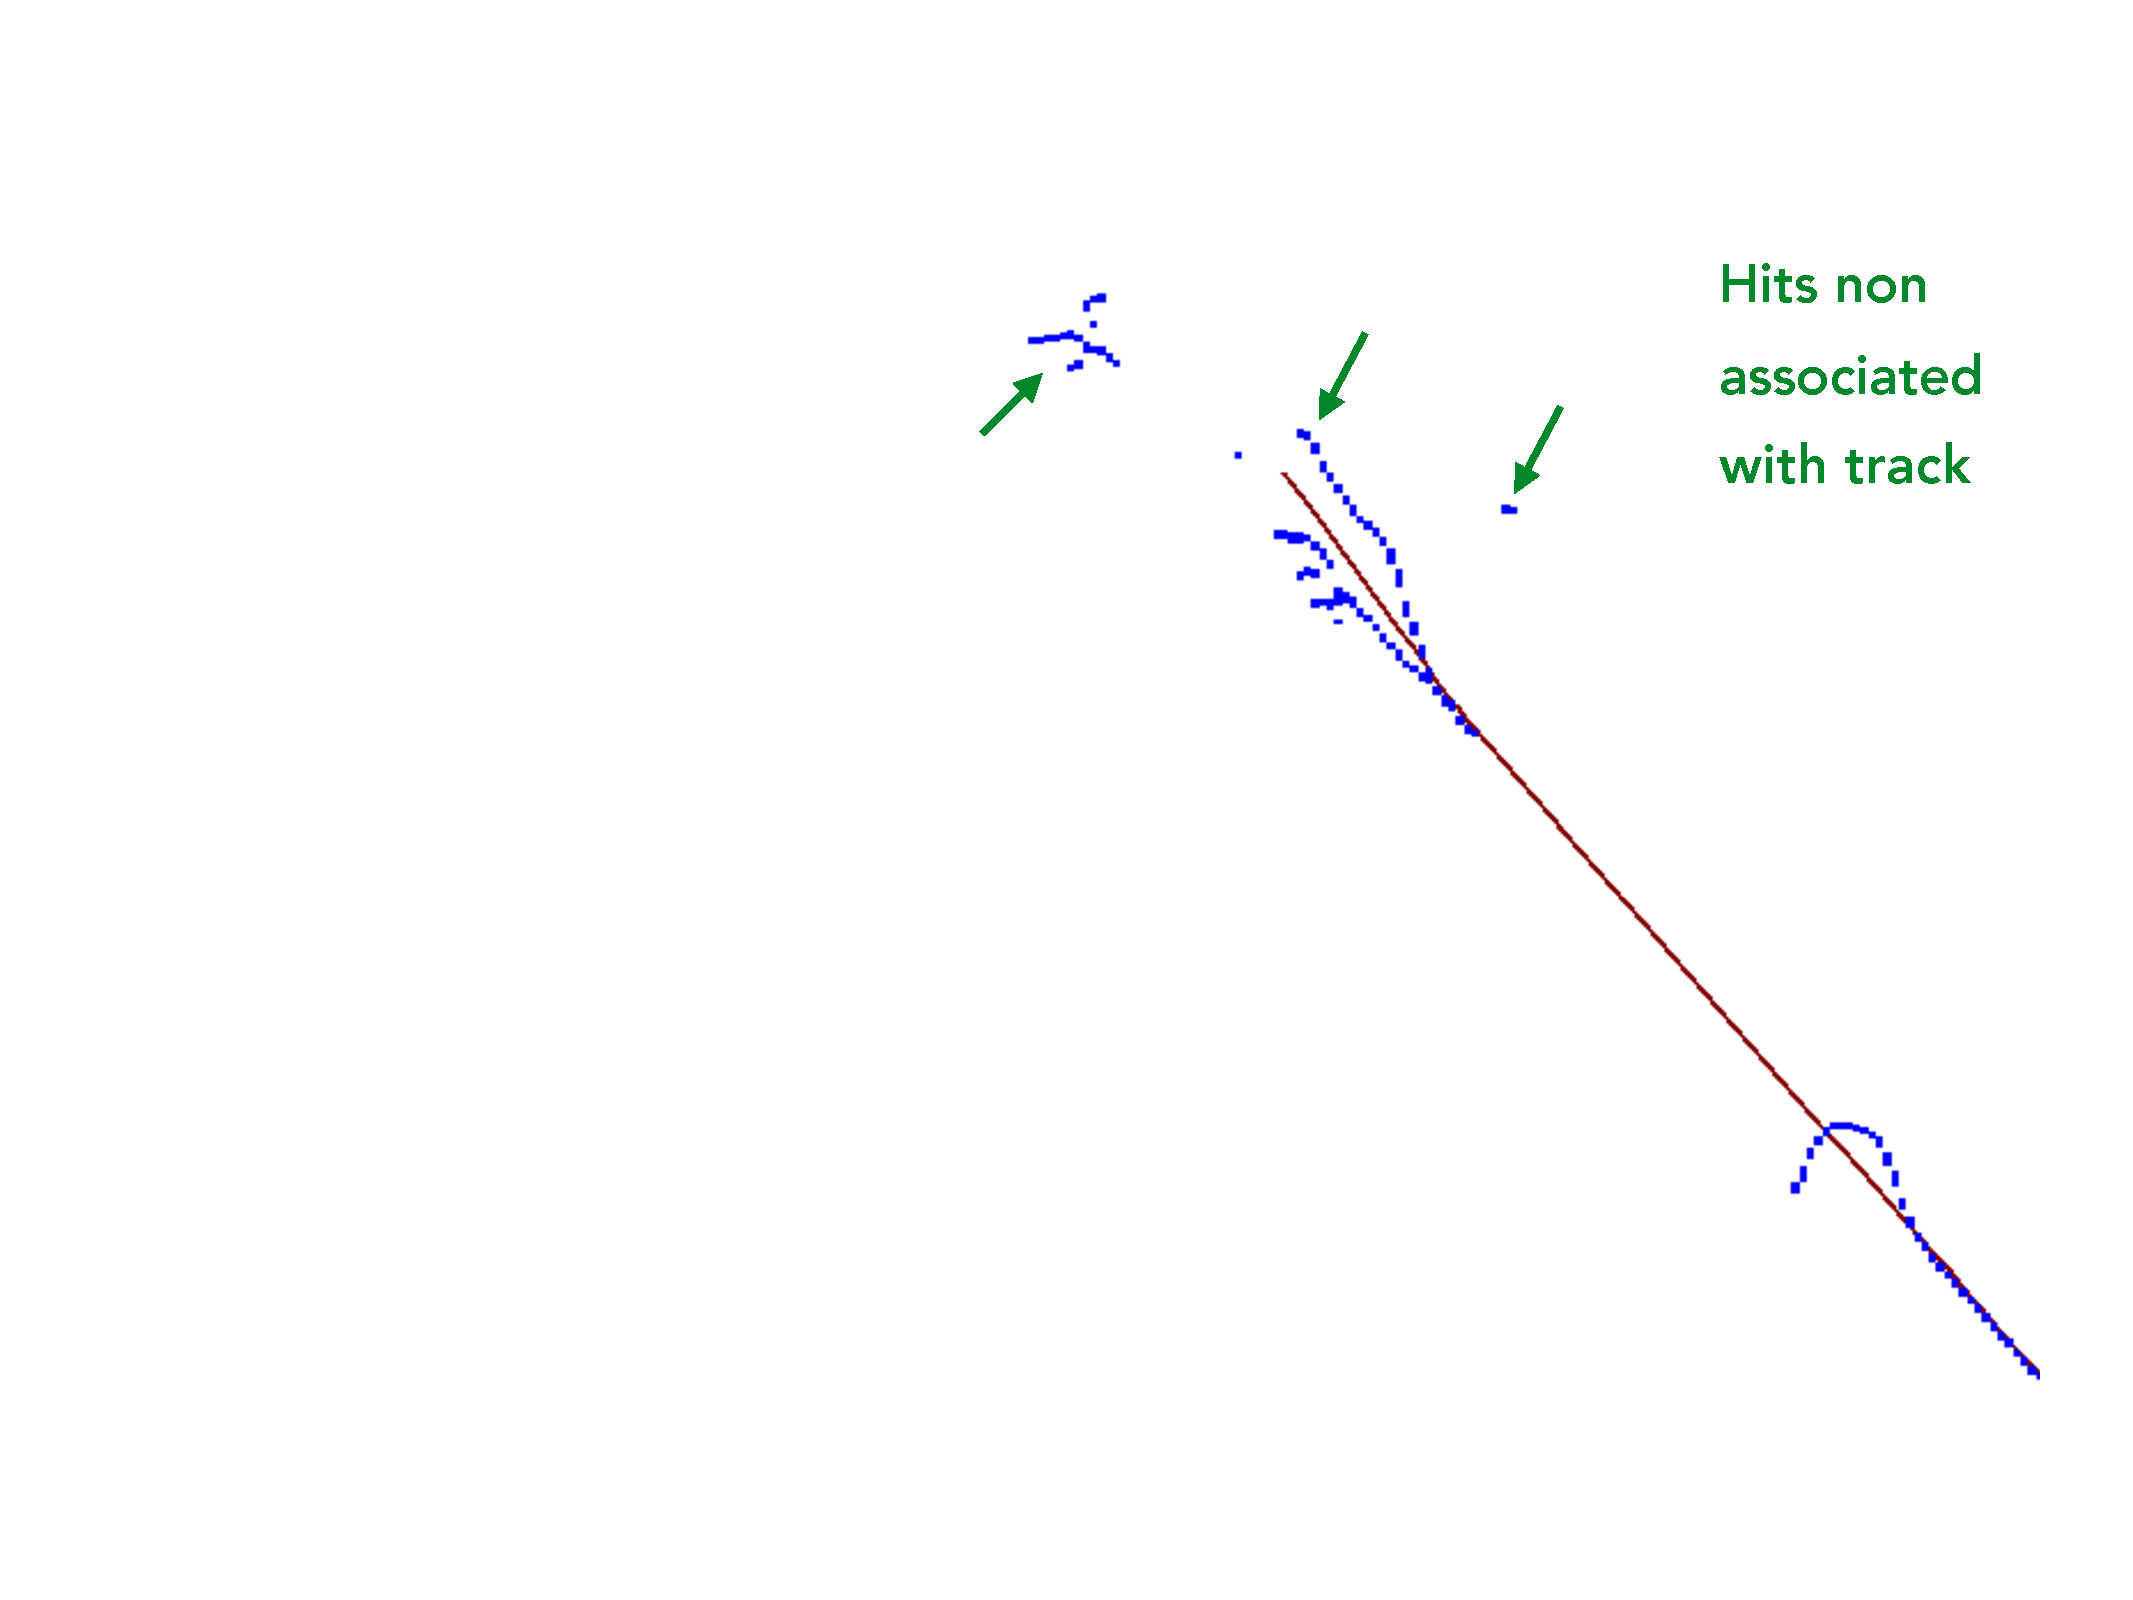
\includegraphics[width=.35\textwidth]{images/figures_hits_not_associated}
   \label{fig:figures_hits_not_associated}} \quad\quad
\subfloat[][]
   {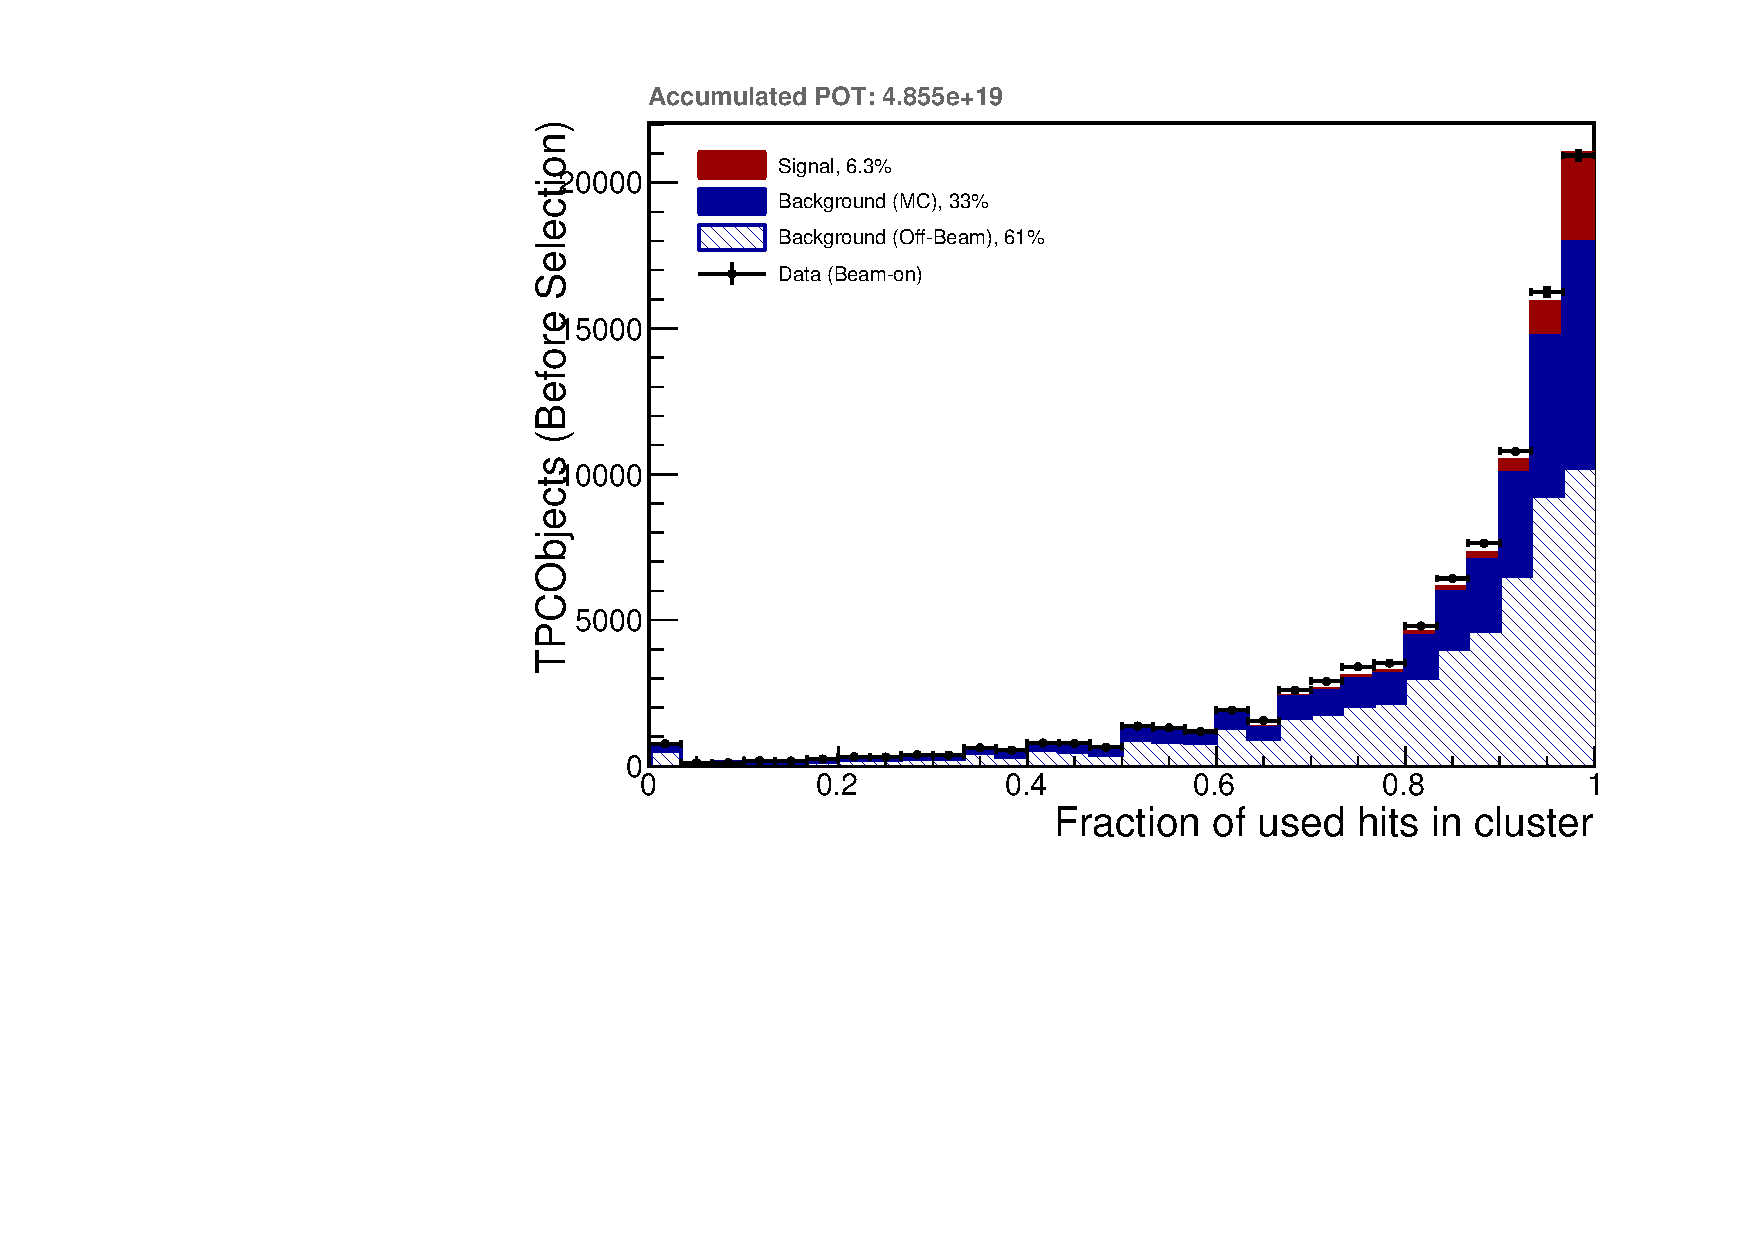
\includegraphics[width=.55\textwidth]{images/aa_frac_used_hits}
   \label{fig:aa_frac_used_hits}} \\ 
\caption[Distribution of Fraction of Used Hits in Clusters]{\protect\subref{fig:figures_hits_not_associated}~Example of simulated shower hits (blue) that were reconstructed as a track (red). All objects are projected onto the collection plane. Some hits (indicated by the green arrows) are not associated to the reconstructed track. 
\protect\subref{fig:aa_frac_used_hits}~Fraction of hits ($f_s$) that are present in the collection plane cluster and that are also associated with a track. A good reconstructed track would have this fraction close to one. Black points are data points. The coloured histograms show the beam-off \acrshort{cr} contribution (hashed), the simulated background (blue) and the simulated $\nu_\mu$ \acrshort{cc} signal events (red).}
\label{fig:aa_trk_quality_frac_used_hits}
\end{figure}

%All these track quality requirements are applied to all tracks in the best flash-matched TPCObject.



%\section[MCS v.s. Length Momentum]{MCS v.s. Length Momentum: Extra Check on Track Quality}
%\label{sec:mcs_lenght_cut}

The quality of a track can also be understood by comparing the \acrshort{mcs} momentum to the range-based momentum (a description of momentum reconstruction is in Section~\ref{sec:momentum_reco}). 
This study can only be performed on tracks spatially contained in the detector since the range-based momentum can only be measured for this kind of tracks.
This comparison is shown in Figure~\ref{fig:aa_mcs_length_2dplot} in a two-dimensional histogram with the \acrshort{mcs} momentum on the $y$ axis and the range-based momentum on the $x$ axis. This distribution shows a linear agreement between the two momentum estimation algorithms, but there are some off-diagonal points. This is better visible in Figure~\ref{fig:aa_mcs_length_1dplot} where the difference between the two momentum estimations is shown. There is a large tail in the positive region due to the mis-reconstructed tracks. Usually, these tracks do not reconstruct the full muon length, and so the range-based momentum is underestimated, but the \acrshort{mcs} momentum is still able to provide a good estimate for the momentum. The comparison between data and simulation for the difference between the two momentum estimations is shown in Figure~\ref{fig:mcs_length_cut_2}. An additional cut is then applied to further reject mis-reconstructed tracks: the \acrshort{mcs} and range-based momenta must agree within 0.2 GeV. 

\begin{figure}[]
\centering
\subfloat[][]
   {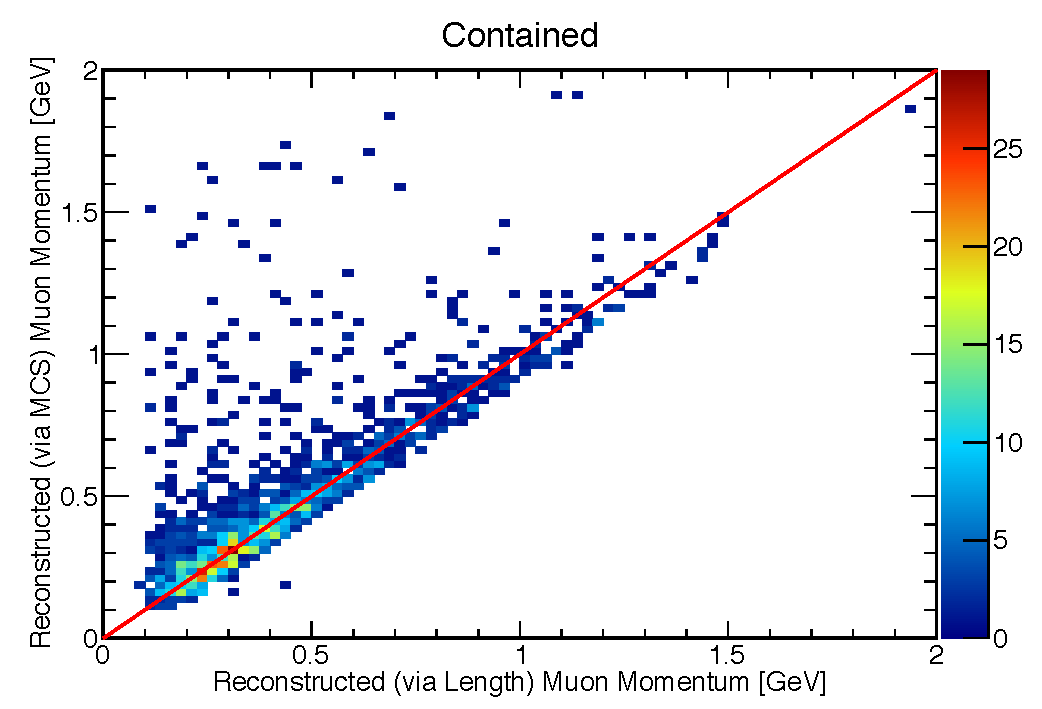
\includegraphics[width=.50\textwidth]{images/MCS/aa_mcs_length_2dplot}
   \label{fig:aa_mcs_length_2dplot}}
\subfloat[][]
   {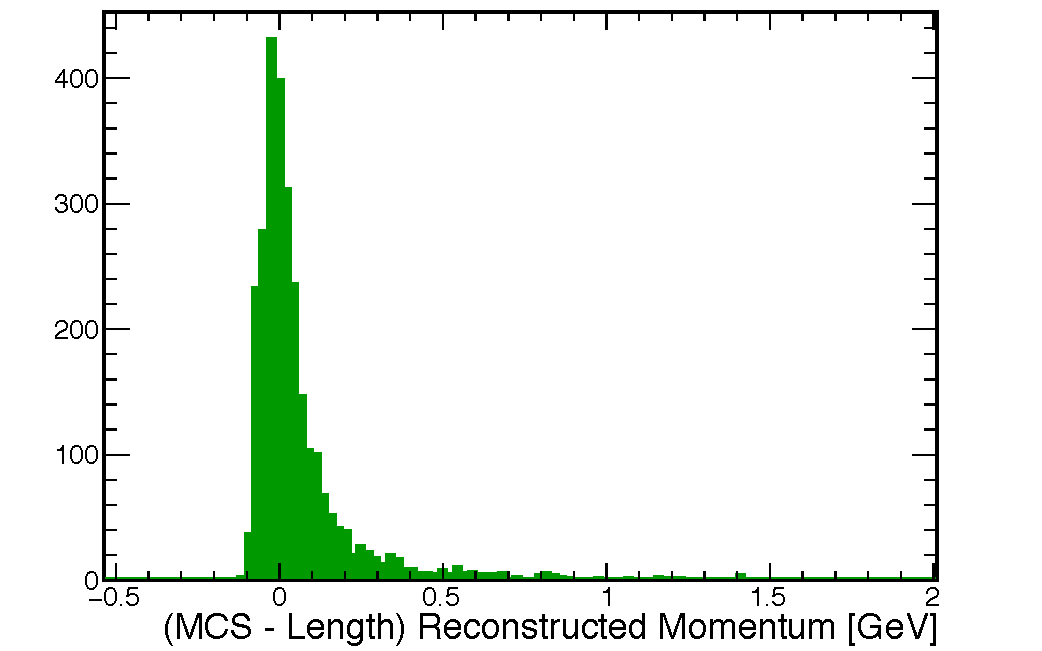
\includegraphics[width=.50\textwidth]{images/MCS/aa_mcs_length_1dplot}
   \label{fig:aa_mcs_length_1dplot}} \\
\caption[\acrshort{mcs} and Range-Based Momentum in Simulation]{\protect\subref{fig:aa_mcs_length_2dplot}~Two-dimensional histogram of the reconstructed muon momentum obtained with the \acrshort{mcs} fit ($y$ axis) and with the range-based algorithm ($x$ axis). \protect\subref{fig:aa_mcs_length_1dplot}~The difference between the two momentum estimations.}
\label{fig:mcs_length_cut}
\end{figure}

\begin{figure}[]
\centering
\subfloat[][Logarithmic scale.]
   {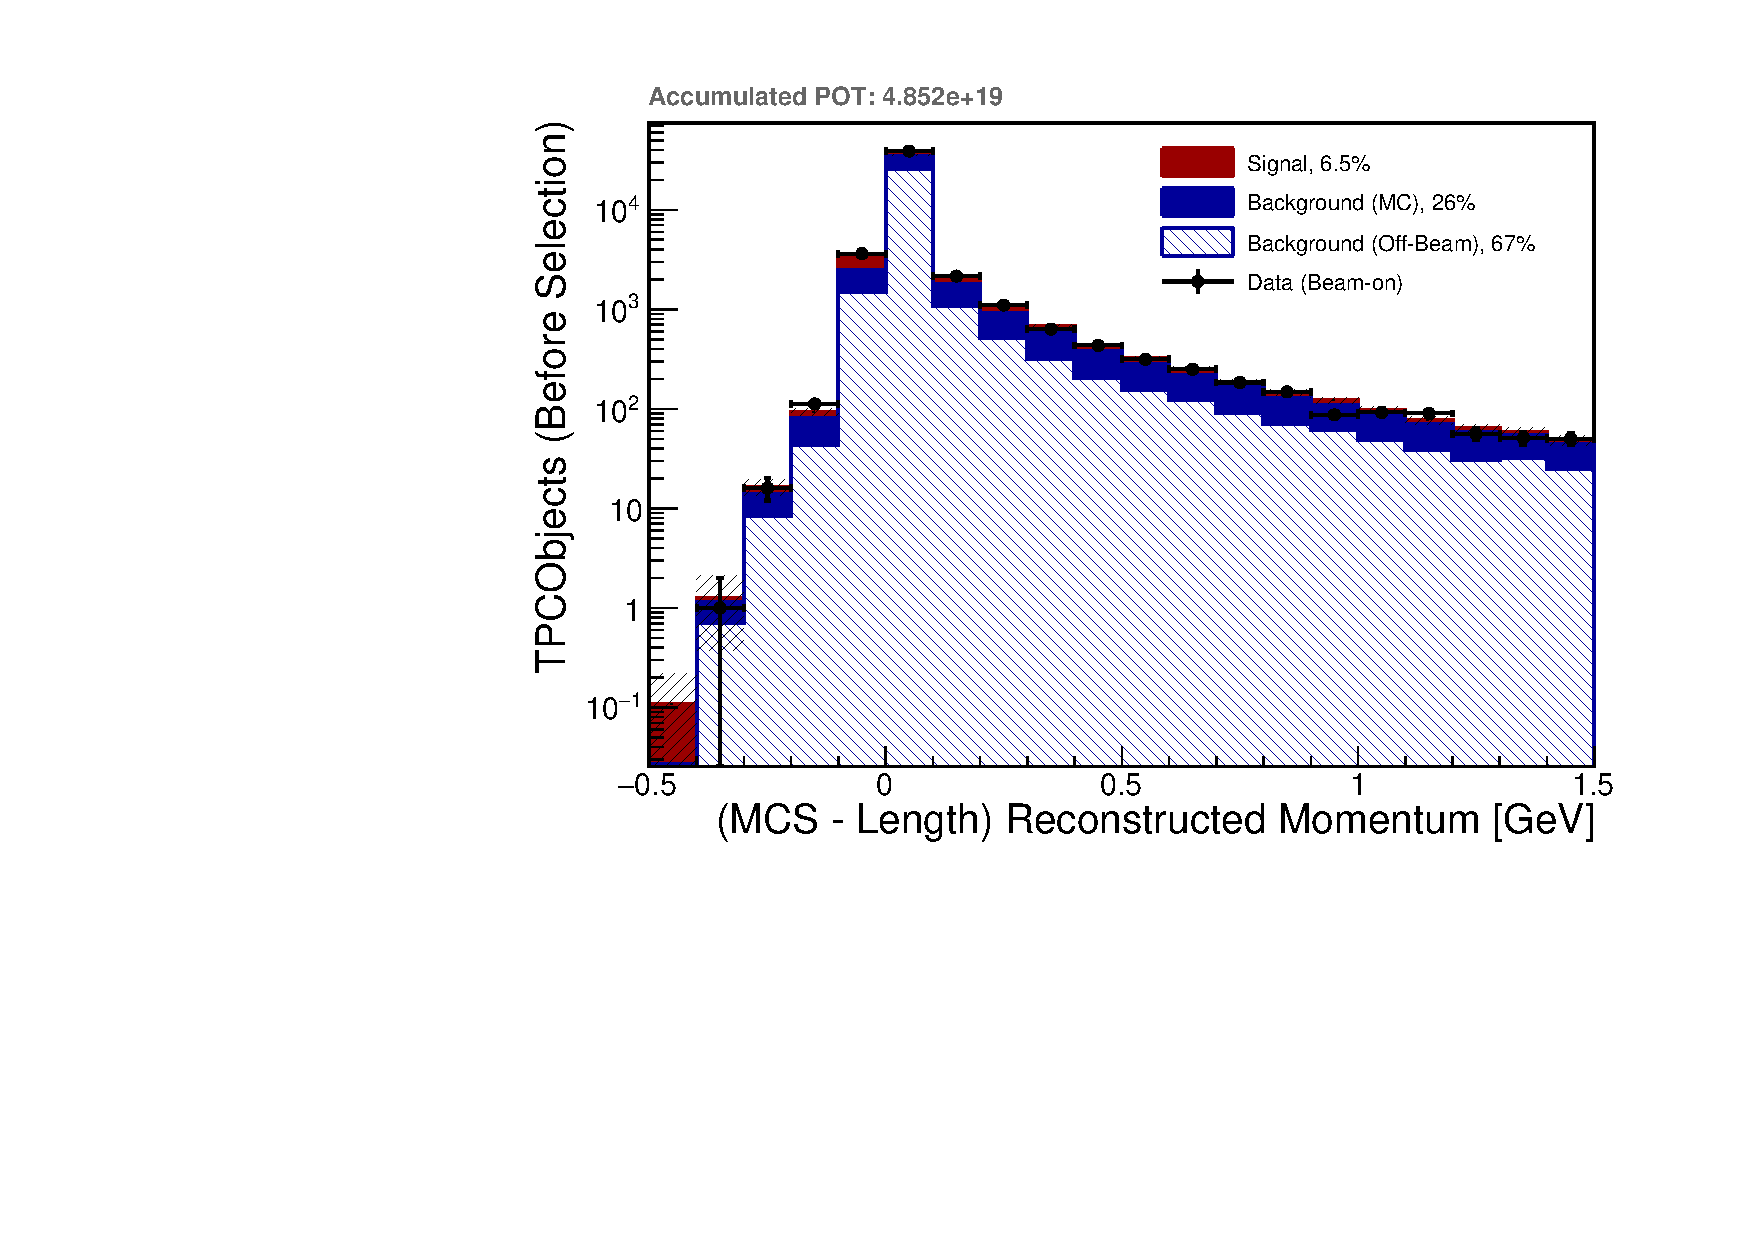
\includegraphics[width=.50\textwidth]{images/MCS/mcs_lenght_log}
   \label{fig:mcs_lenght_log}}
\subfloat[][Linear scale, enlarged in the cut region.]
   {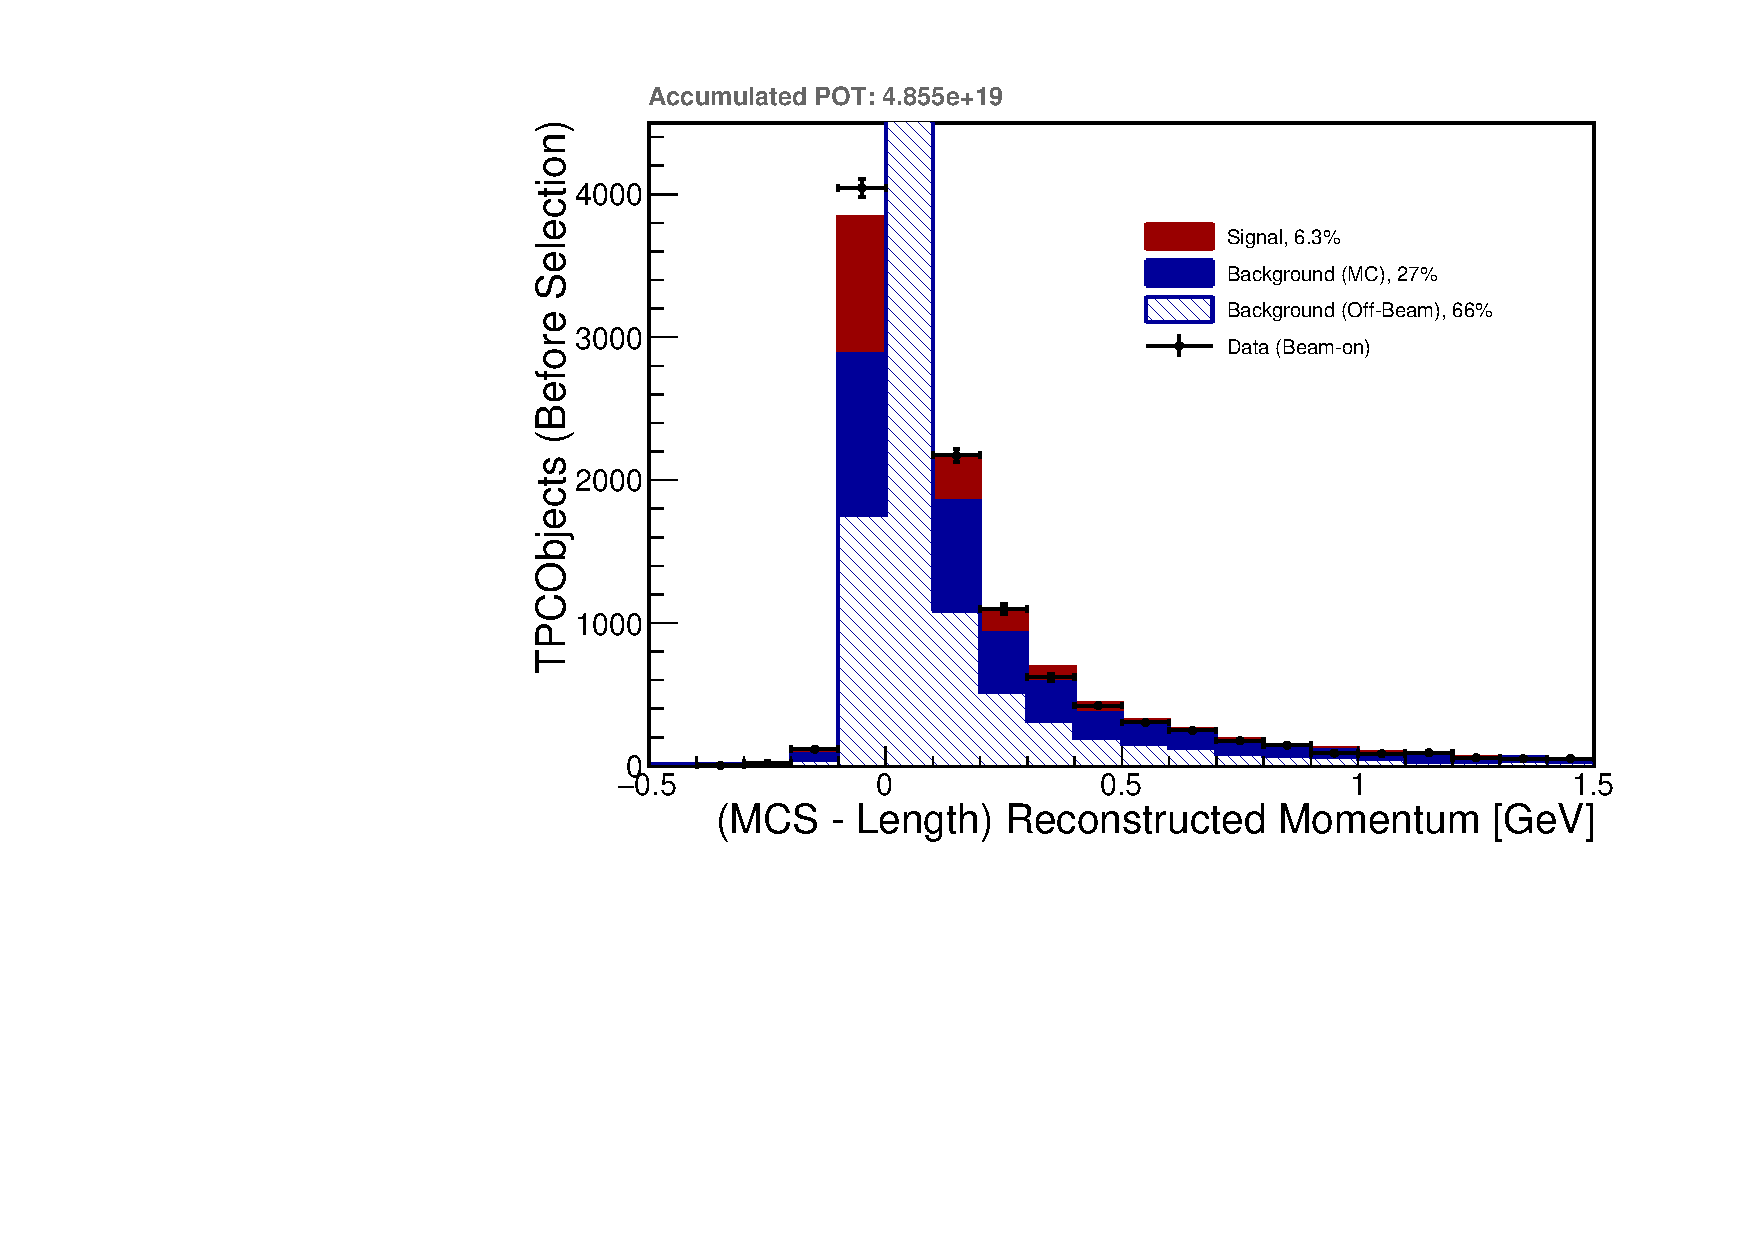
\includegraphics[width=.50\textwidth]{images/MCS/aa_mcs_length}
   \label{fig:aa_mcs_length}} \\
\caption[\acrshort{mcs} and Range-Based Momentum in Data]{Similar plot to \ref{fig:aa_mcs_length_1dplot}, but this time showing the simulation with the beam-off data (shaded) compared to beam-on data. Plots are \acrshort{pot} normalised. Plot~\protect\subref{fig:mcs_lenght_log} is in logarithmic scale, while plot~\protect\subref{fig:aa_mcs_length} is in linear scale and has been enlarged in the region where the cut is placed (0.2 GeV). The coloured histograms show the beam-off \acrshort{cr} contribution (hashed), the simulated background (blue) and the simulated $\nu_\mu$ \acrshort{cc} signal events (red).}
\label{fig:mcs_length_cut_2}
\end{figure}




\section{Fiducial Volume}
\label{sec:fiducial_volume}

A \acrshort{fv} is chosen in order to reduce the amount of  \acrshort{cr} muons contamination and also to remove unresponsive detector regions. The \acrshort{fv}, shown in Figure~\ref{fig:fiducial_volume} and is a rectangular parallelepiped whose faces are located at a distance of 35 cm from the top and bottom \acrshort{tpc} faces. It is defined in order to remove \acrshort{cr}s whose start and end positions are either misplaced by the space-charge effect or by mis-reconstruction issues. The \acrshort{fv} faces are also 25 cm distant from the front face and 85 cm from the end of the detector, to reject muons interacting in the very end of the \acrshort{tpc} that would not leave a substantial track, as they would be exiting immediately. In the drift direction, the faces are 12 cm distant. There is a 100 cm gap along the beam ($z$) direction that divides the \acrshort{fv} in two regions. This is done to exclude a region in the collection plane with unresponsive wires.

\begin{figure}[t]
\centering
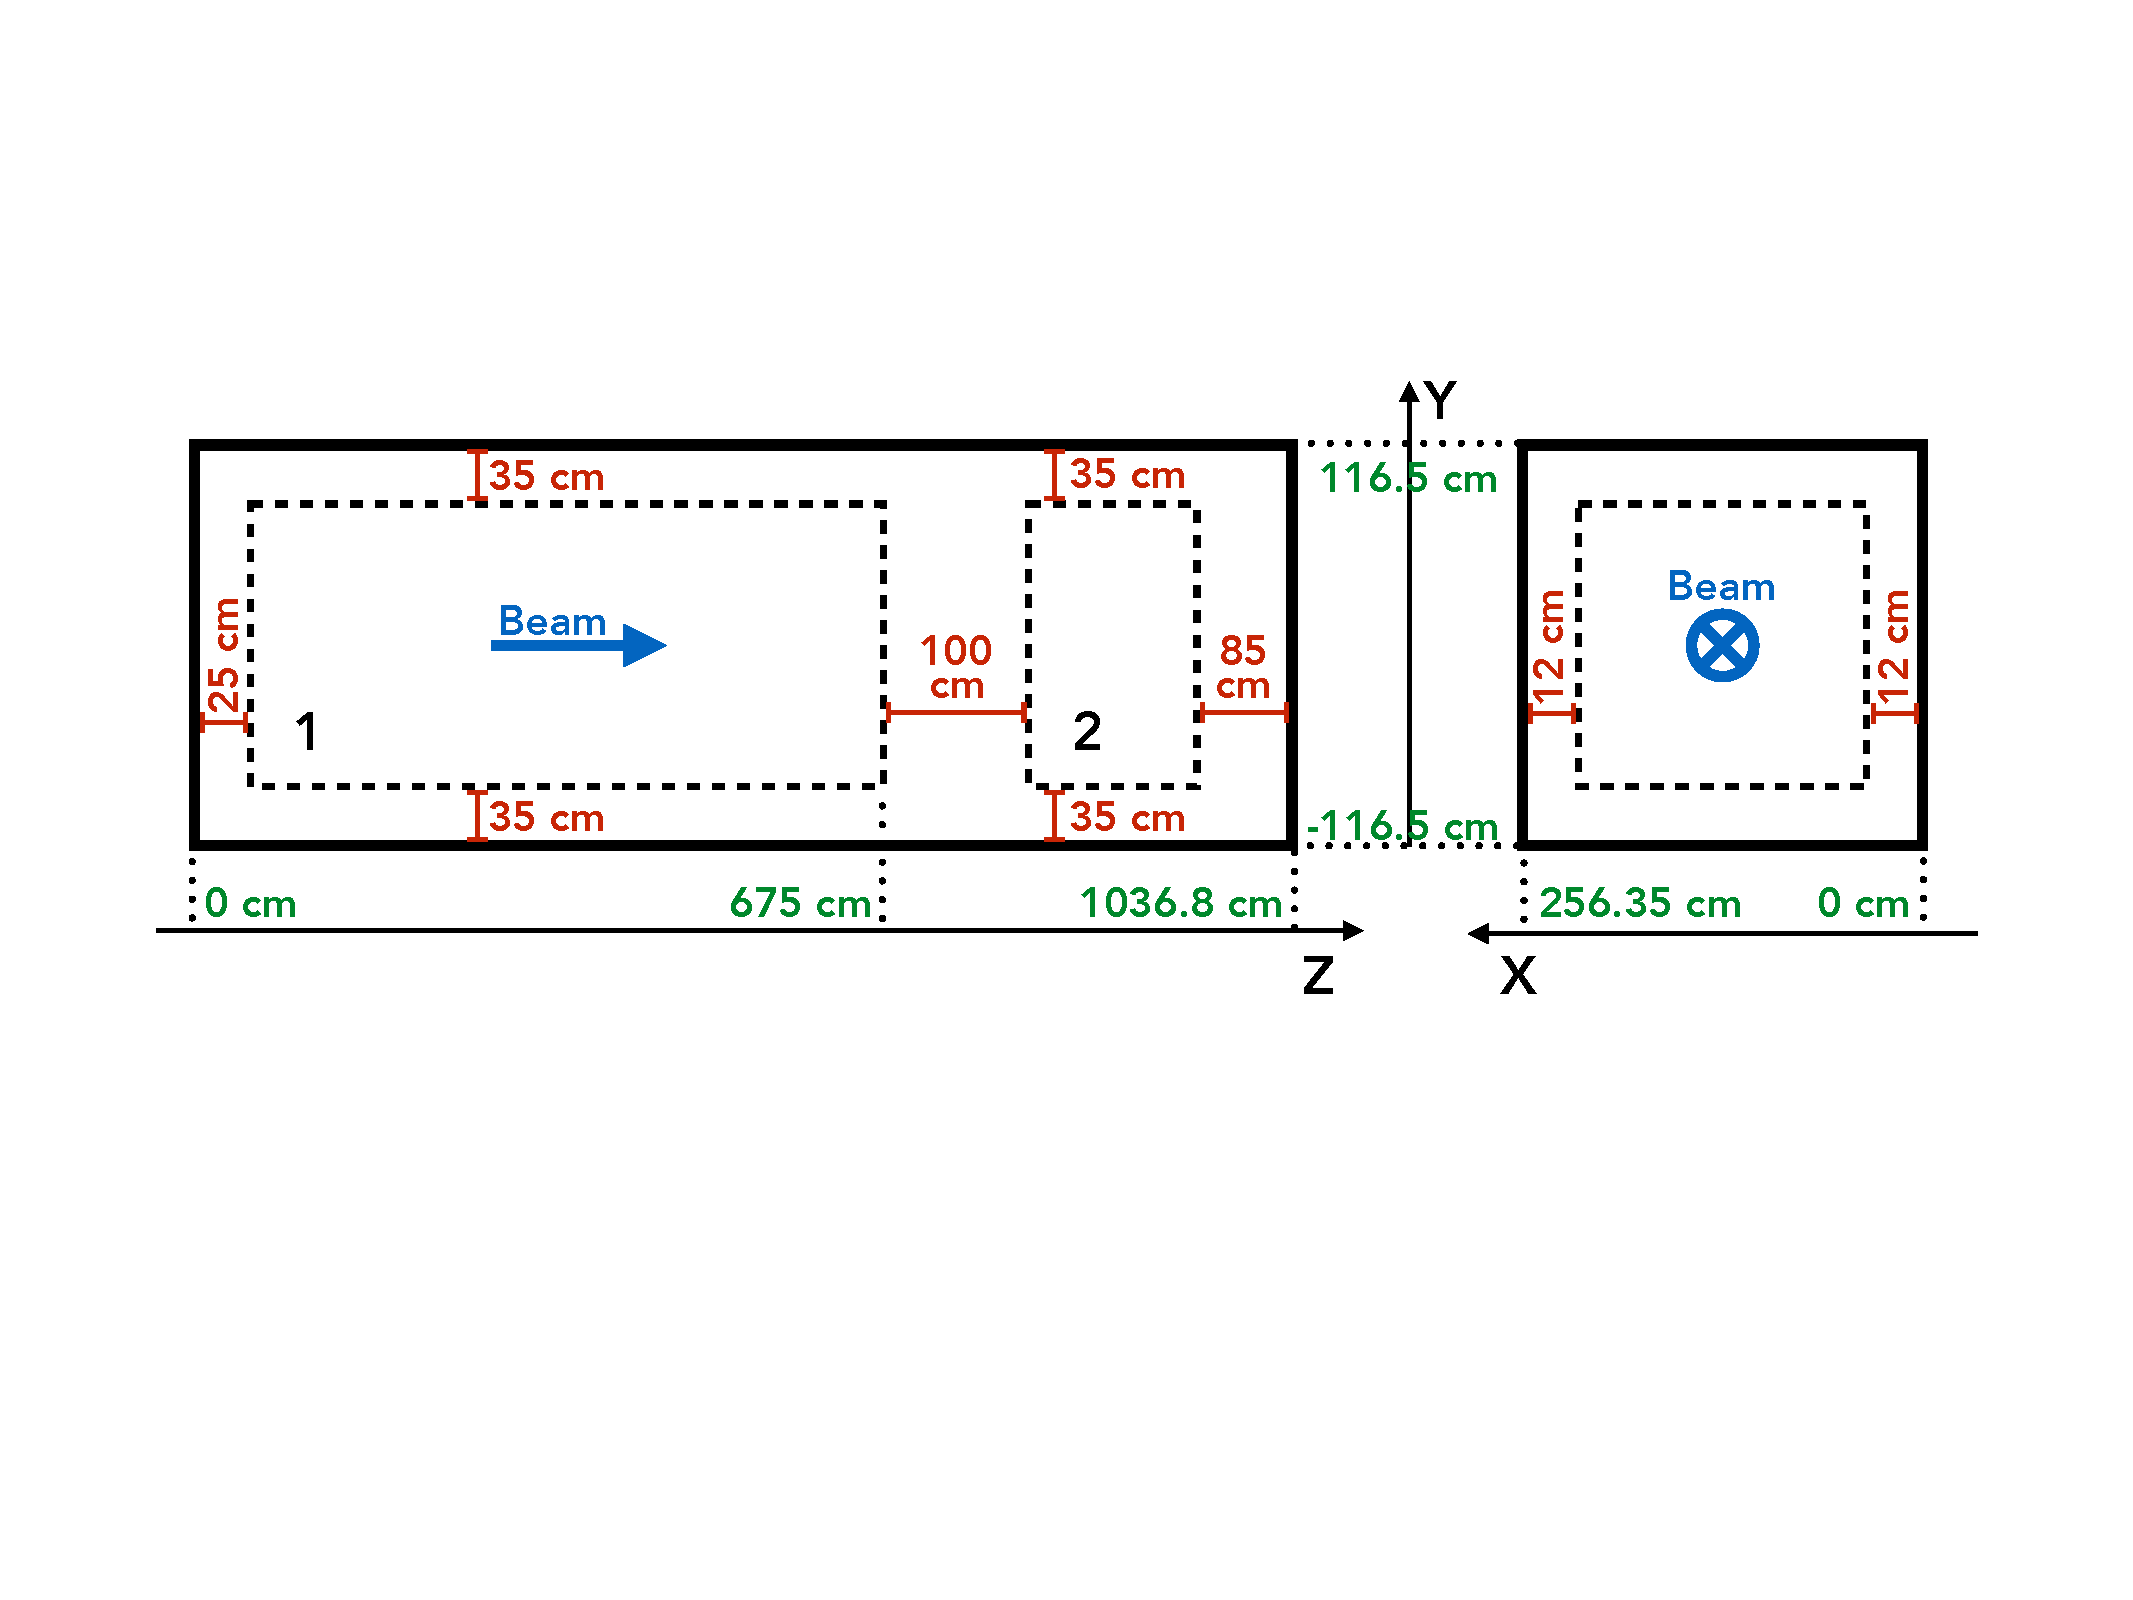
\includegraphics[width=.95\textwidth]{images/fiducial_volume}
\caption[Fiducial Volume]{The \acrshort{fv} used for this analysis. The solid black line is a schematic of the \acrshort{tpc}. The \acrshort{fv} is shown with a dashed line.}
\label{fig:fiducial_volume}
\end{figure}

As a final cut in the event selection, the reconstructed neutrino vertex is required to be in the aforementioned \acrshort{fv}.



\section{Selected Event Distributions}
\label{sec:event_distributions}

Figure~\ref{fig:final_dist} shows the distributions of the most relevant variables of the selected candidate muon track. The data distributions are compared with the two different \g configurations described in Section~\ref{sec:simulation}. However, only the ``\tuneone'' simulation, being the default MicroBooNE simulation,  will be used for the cross section extraction. The distributions shown are:
\begin{itemize} 
\item the measured muon momentum $p_\mu$ in \subref{fig:trkmom_tune1} and \subref{fig:trkmom_tune3},
\item the measured cosine of the muon angle with respect to the beamline $\cos\theta_\mu$ in \subref{fig:trkcostheta_tune1} and \subref{fig:trkcostheta_tune3},
\item the muon track length in \subref{fig:trklen_tune1} and \subref{fig:trklen_tune3},
\item the muon angle around the beamline $\phi$ in \subref{fig:trkphi_tune1} and \subref{fig:trkphi_tune3},
\item the number of reconstructed particles coming from the neutrino interaction vertex in \subref{fig:multpfp_tune1} and \subref{fig:multpfp_tune3},
%\item the number of track-like particles coming from the neutrino interaction vertex in \subref{fig:multtracktol_tune1} and \subref{fig:multtracktol_tune3},
\item the neutrino reconstructed vertex along the drift direction $x$ in \subref{fig:vtxx_tune1} and \subref{fig:vtxx_tune3},
\item the neutrino reconstructed vertex along the vertical direction $y$ in \subref{fig:vtxy_tune1} and \subref{fig:vtxy_tune3},
\item the neutrino reconstructed vertex along the neutrino beam direction $z$ in \subref{fig:vtxz_tune1} and \subref{fig:vtxz_tune3}.
\end{itemize}
The angle definitions are shown in Figure~\ref{fig:coord_system} for reference. The black data points represent beam-on data with statistical uncertainties only shown with vertical bars. Beam-off data is also shown with an hashed histogram, and is stacked together with simulated events, as described in Section~\ref{sec:simulation}. The data correspond to $1.592 \times 10^{20}$ \acrshort{pot}.
%
\begin{figure}[]
\centering
\subfloat[][\tuneone.]
   {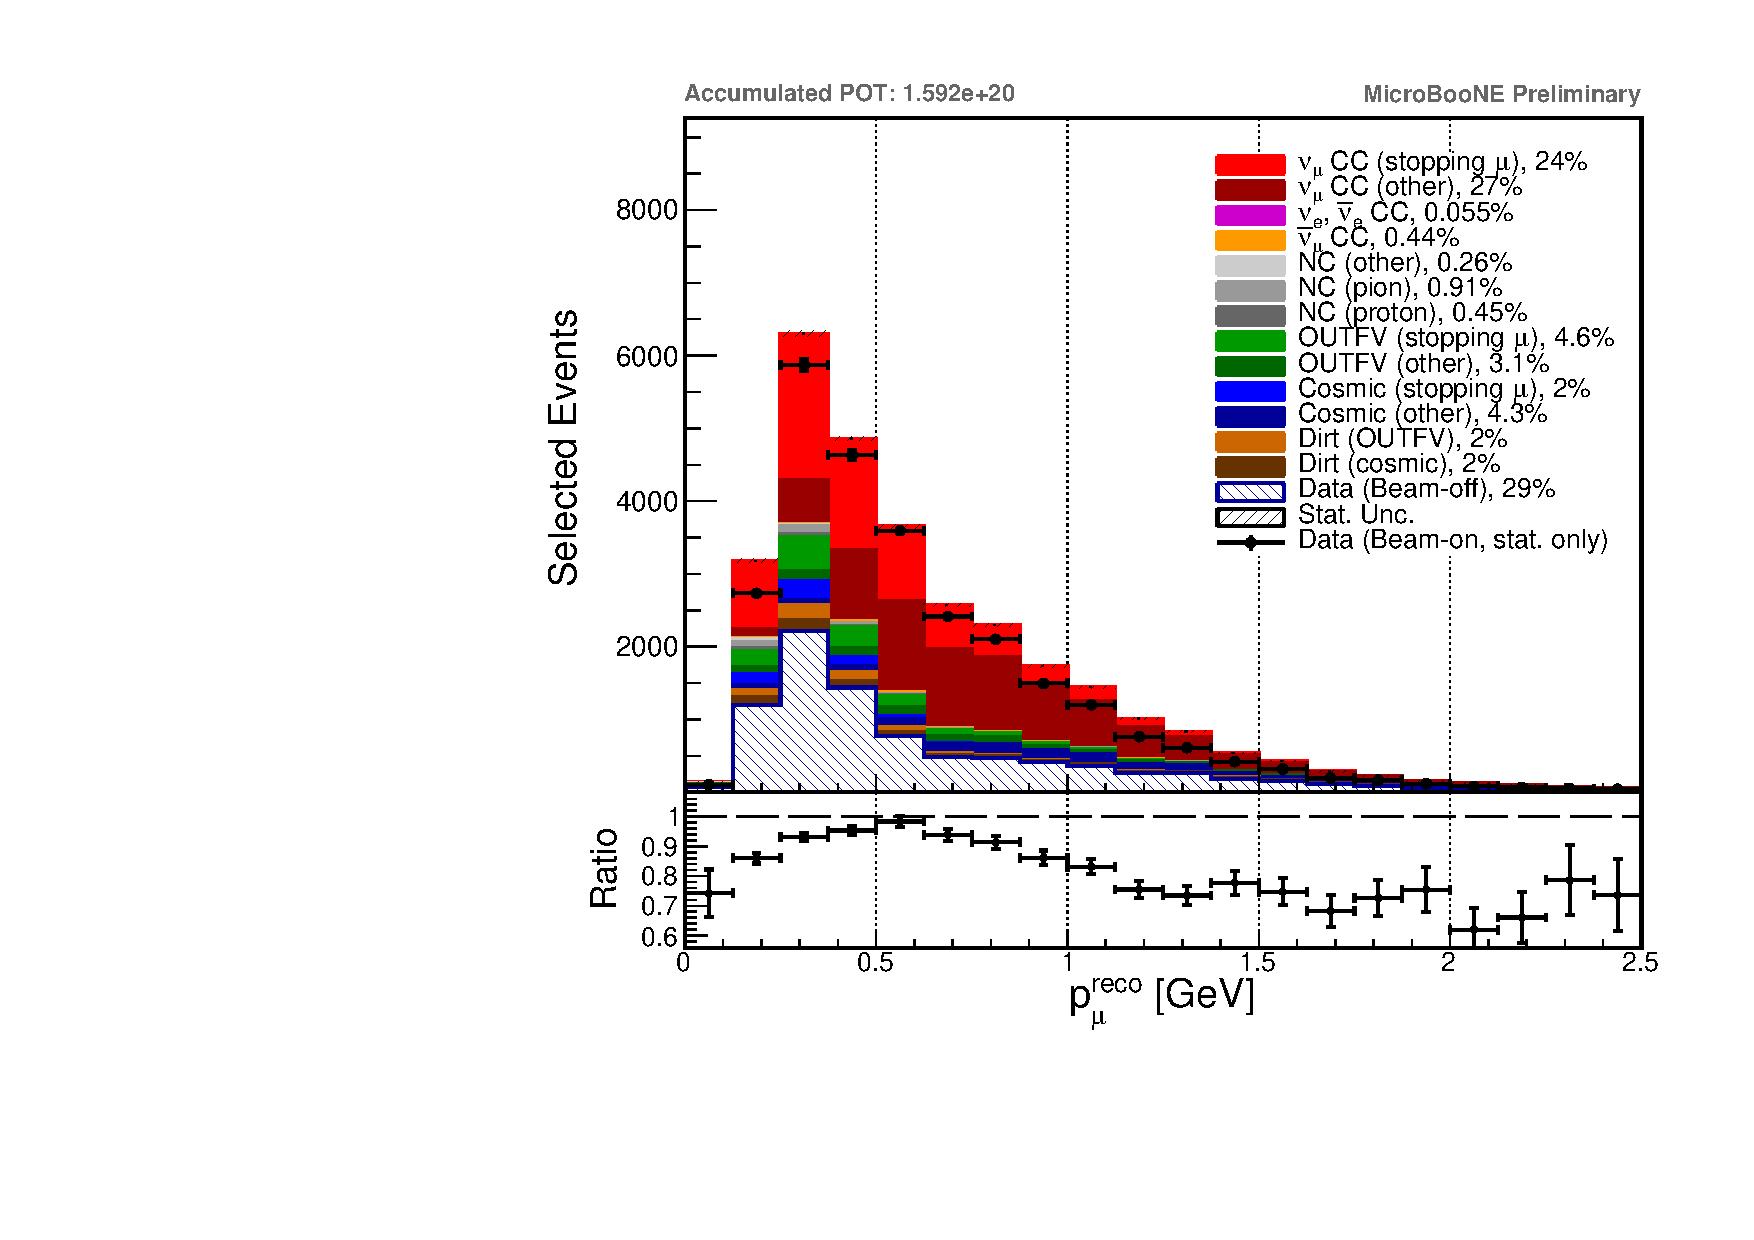
\includegraphics[width=.45\textwidth]{images/DataMC_Tune1/trkmom_tune1}
   \label{fig:trkmom_tune1}} \quad
\subfloat[][\tunethree.]
   {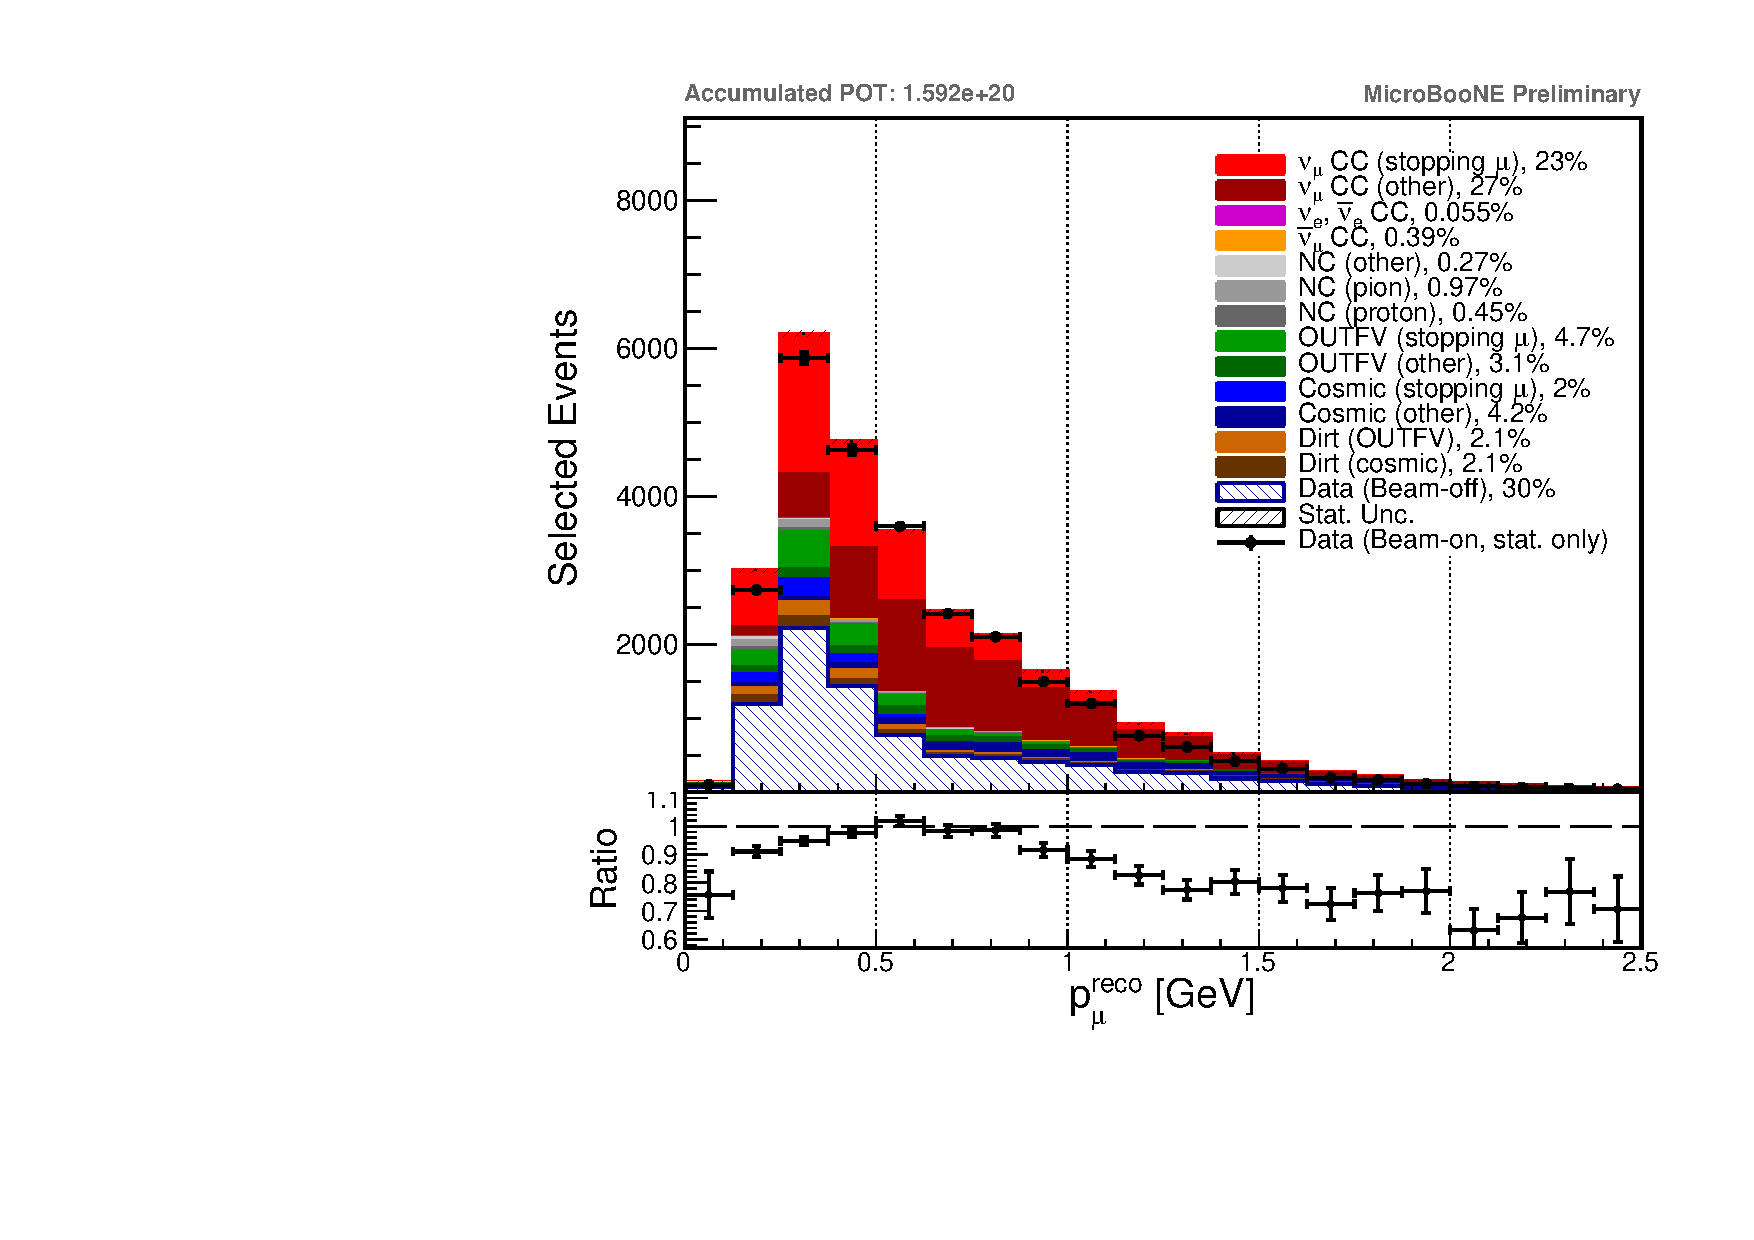
\includegraphics[width=.45\textwidth]{images/DataMC_Tune3/trkmom_tune3}
   \label{fig:trkmom_tune3}} \quad
\subfloat[][\tuneone.]
   {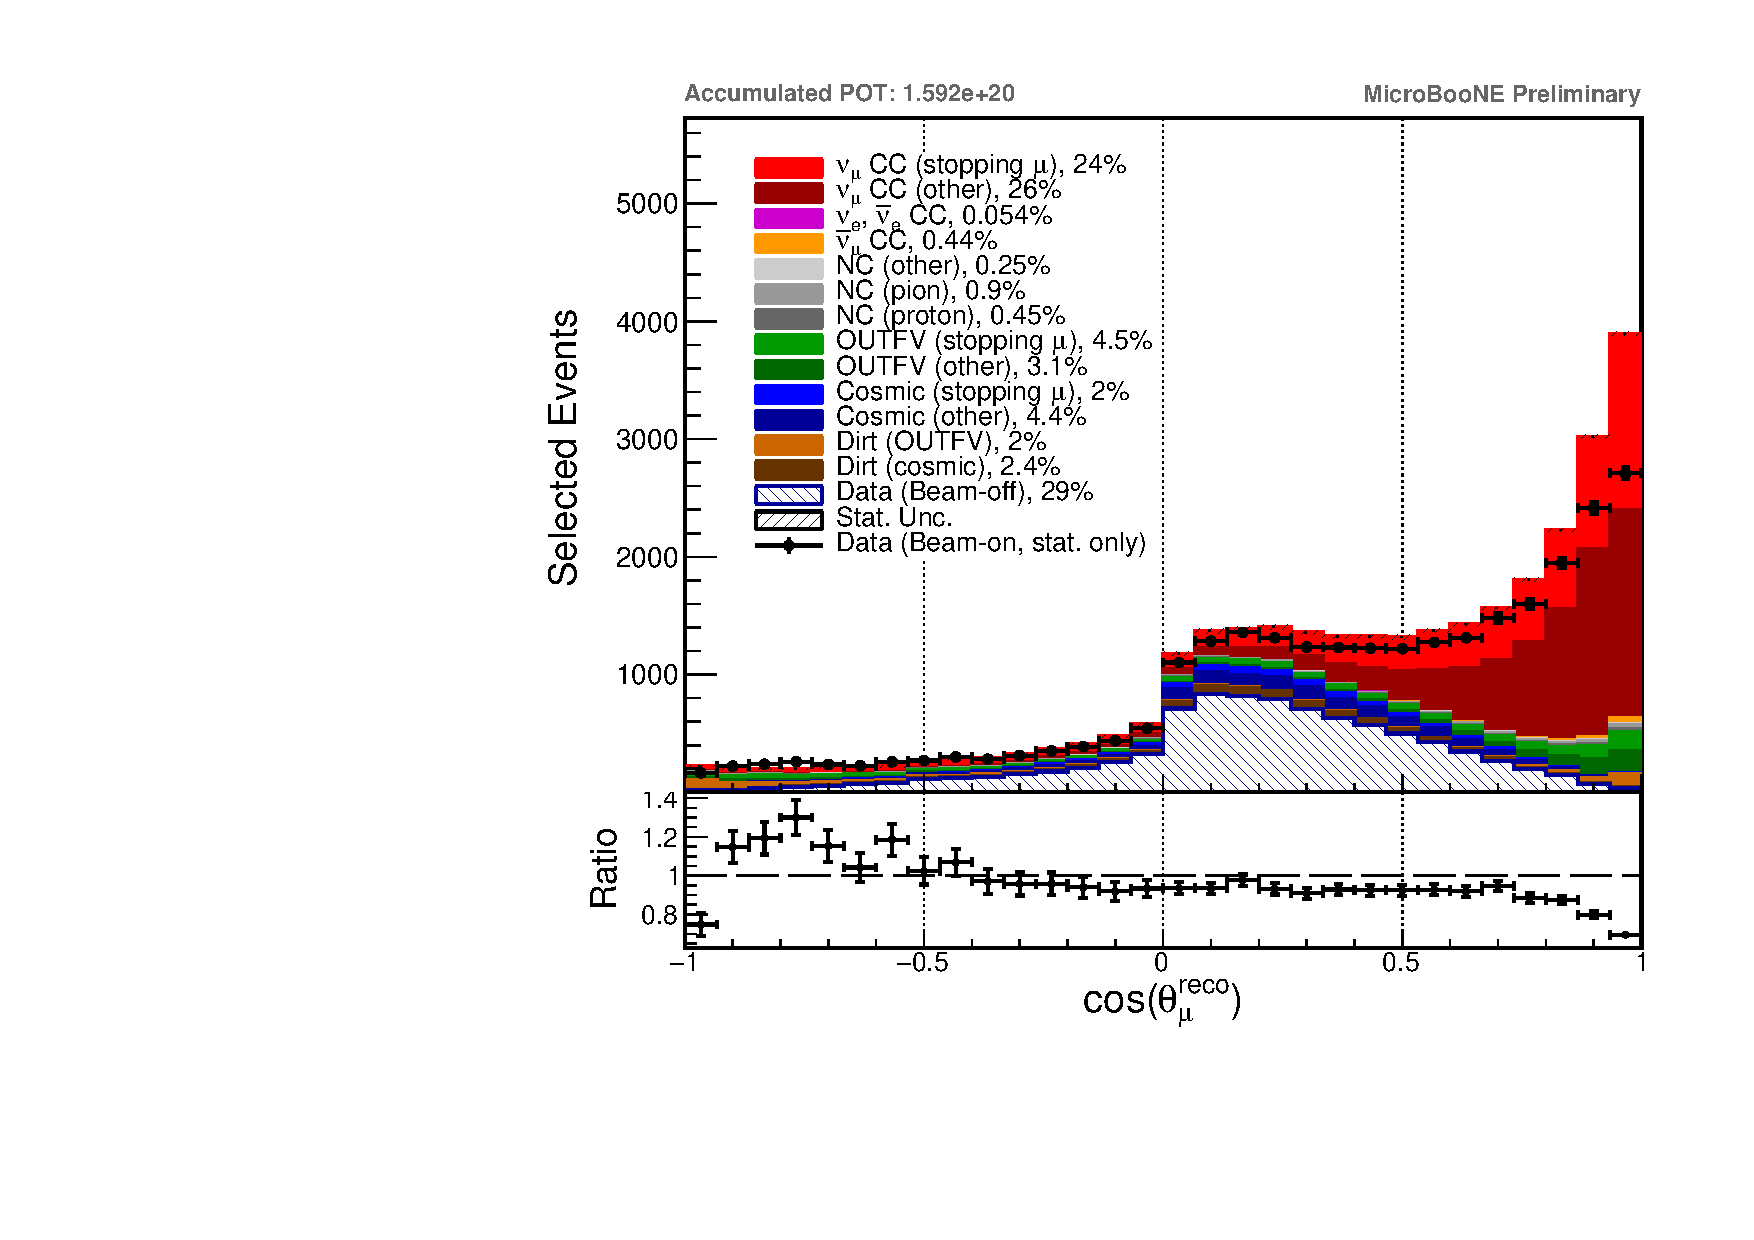
\includegraphics[width=.45\textwidth]{images/DataMC_Tune1/trkcostheta_tune1}
   \label{fig:trkcostheta_tune1}} \quad
\subfloat[][\tunethree.]
   {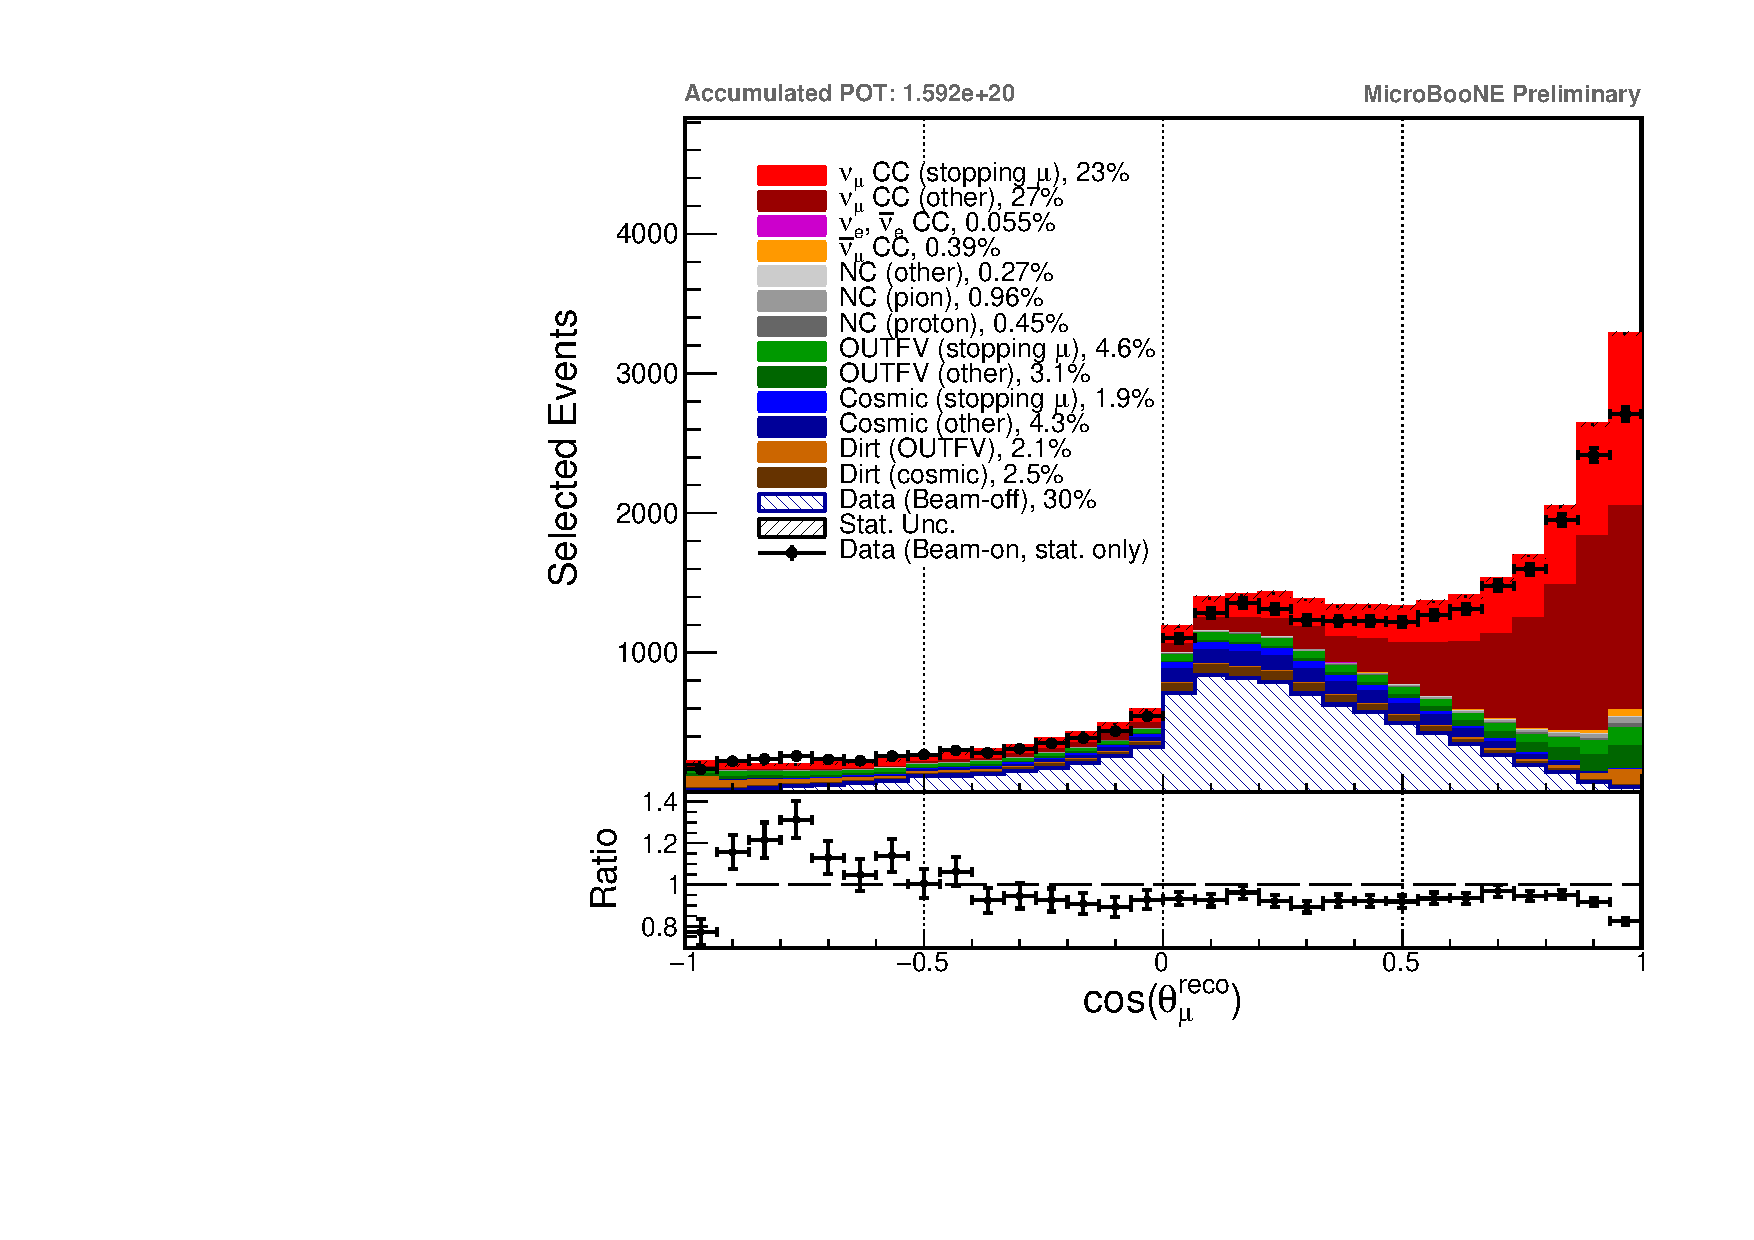
\includegraphics[width=.45\textwidth]{images/DataMC_Tune3/trkcostheta_tune3}
   \label{fig:trkcostheta_tune3}} \quad
\subfloat[][\tuneone.]
   {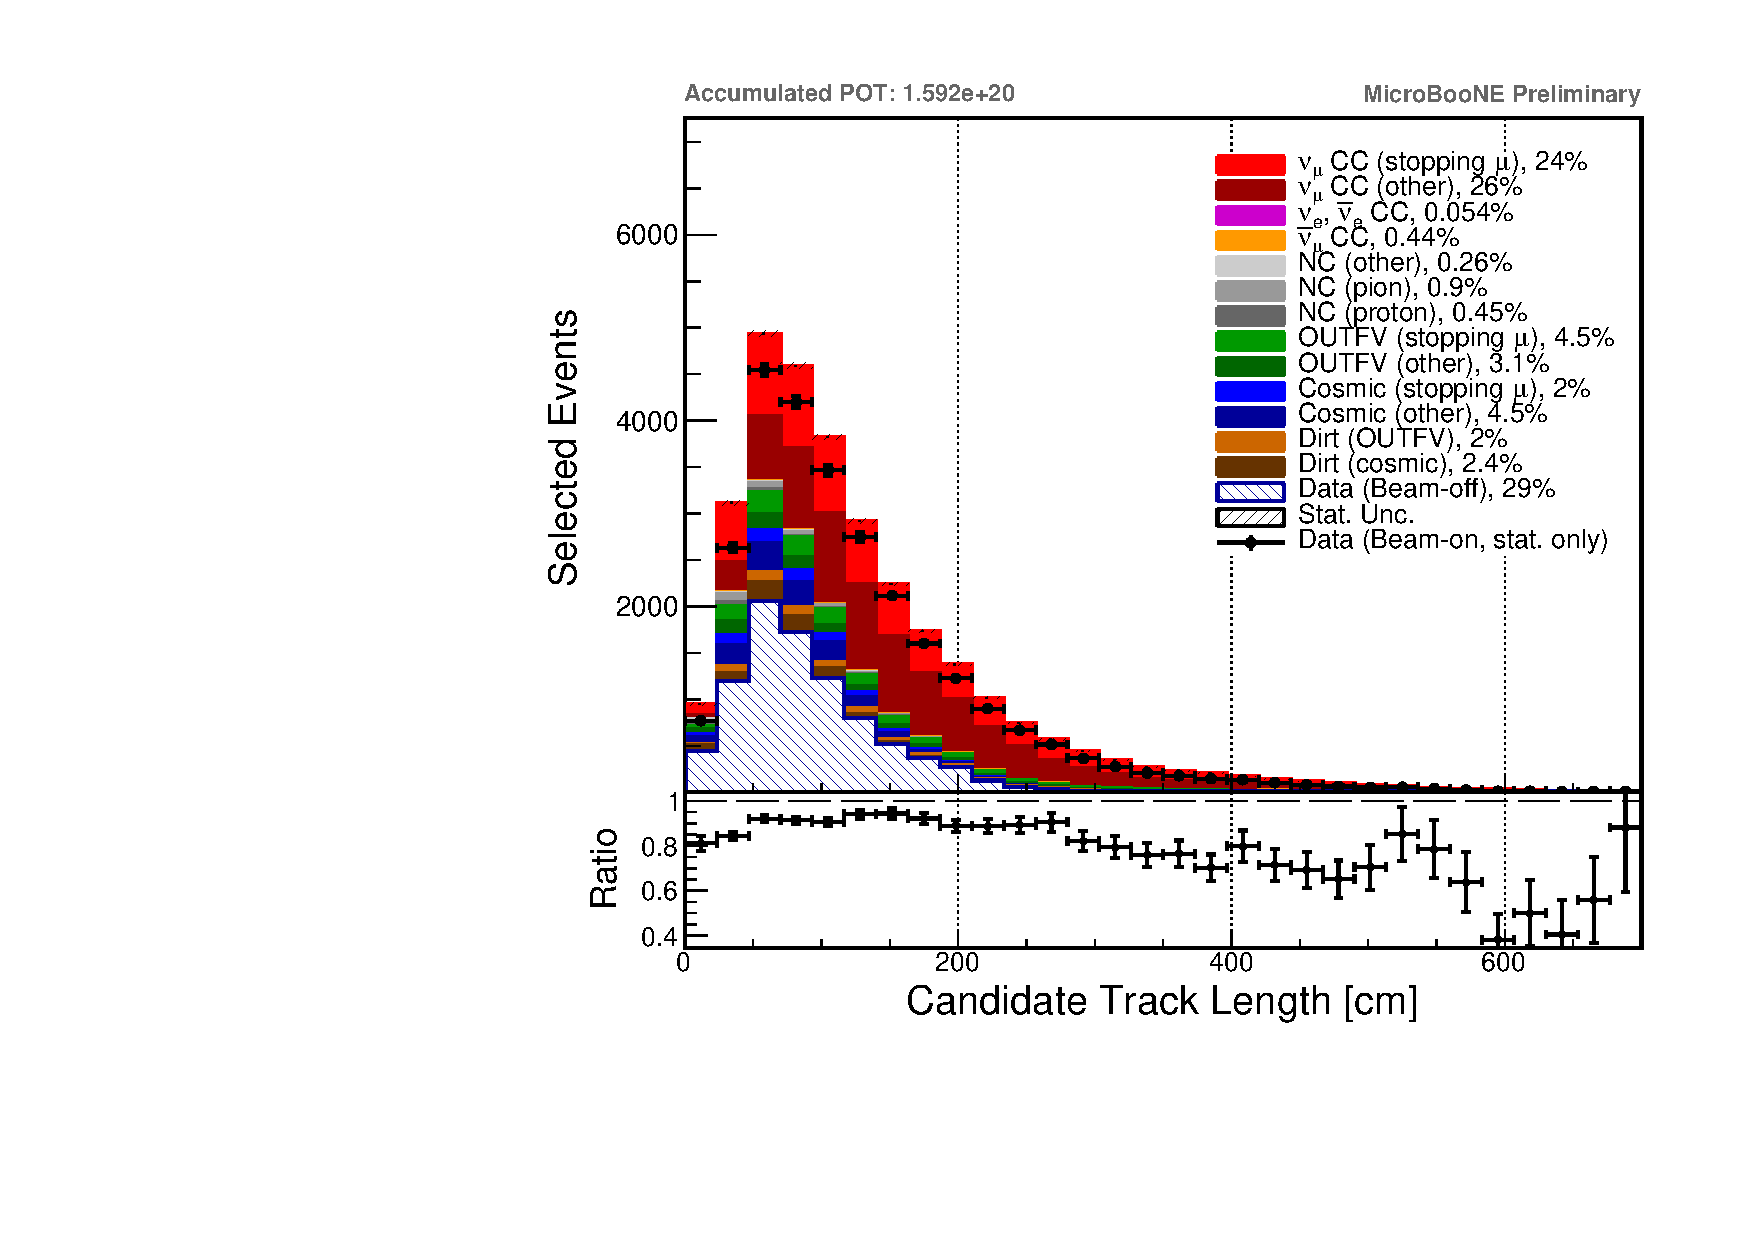
\includegraphics[width=.45\textwidth]{images/DataMC_Tune1/trklen_tune1}
   \label{fig:trklen_tune1}} \quad
\subfloat[][\tunethree.]
   {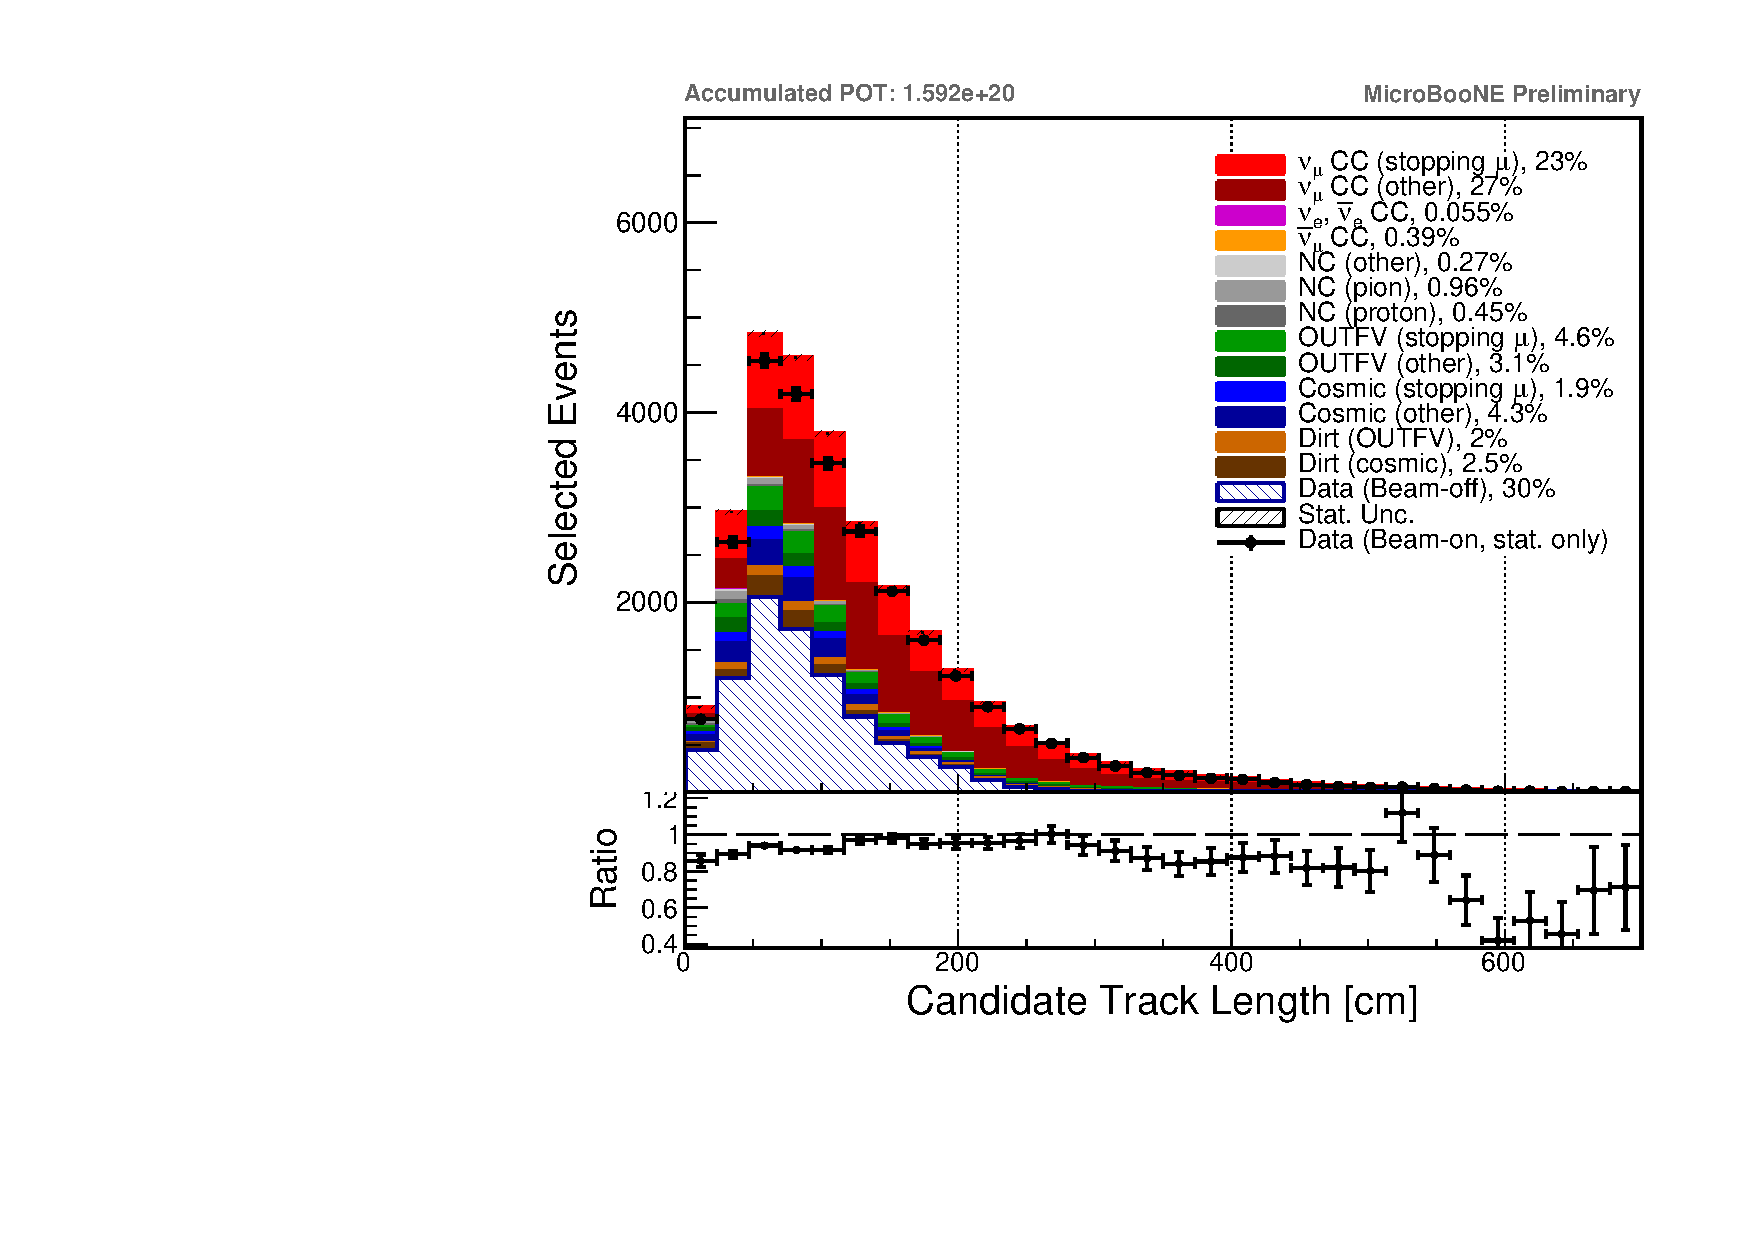
\includegraphics[width=.45\textwidth]{images/DataMC_Tune3/trklen_tune3}
   \label{fig:trklen_tune3}} \quad
\caption[Distribution of Selected Events ($p_\mu$, $\cos\theta_\mu$, $l$)]{Event distributions of the selected events. The black data points symbolise beam-on data with statistical uncertainties. The stacked coloured histograms represent the simulation, with the shaded bands representing the statistical uncertainty only. The red histograms shows the signal events. The hashed histogram is beam-off data. Data and \acrshort{mc} correspond to $1.592 \times 10^{20}$ \acrshort{pot}. Left plots show \acrshort{mc} from the ``\tuneone'' configuration, right ones from the ``\tunethree'' configuration.}
\label{fig:final_dist}
\end{figure}
%
\begin{figure}[]
\ContinuedFloat
\centering
\subfloat[][\tuneone.]
   {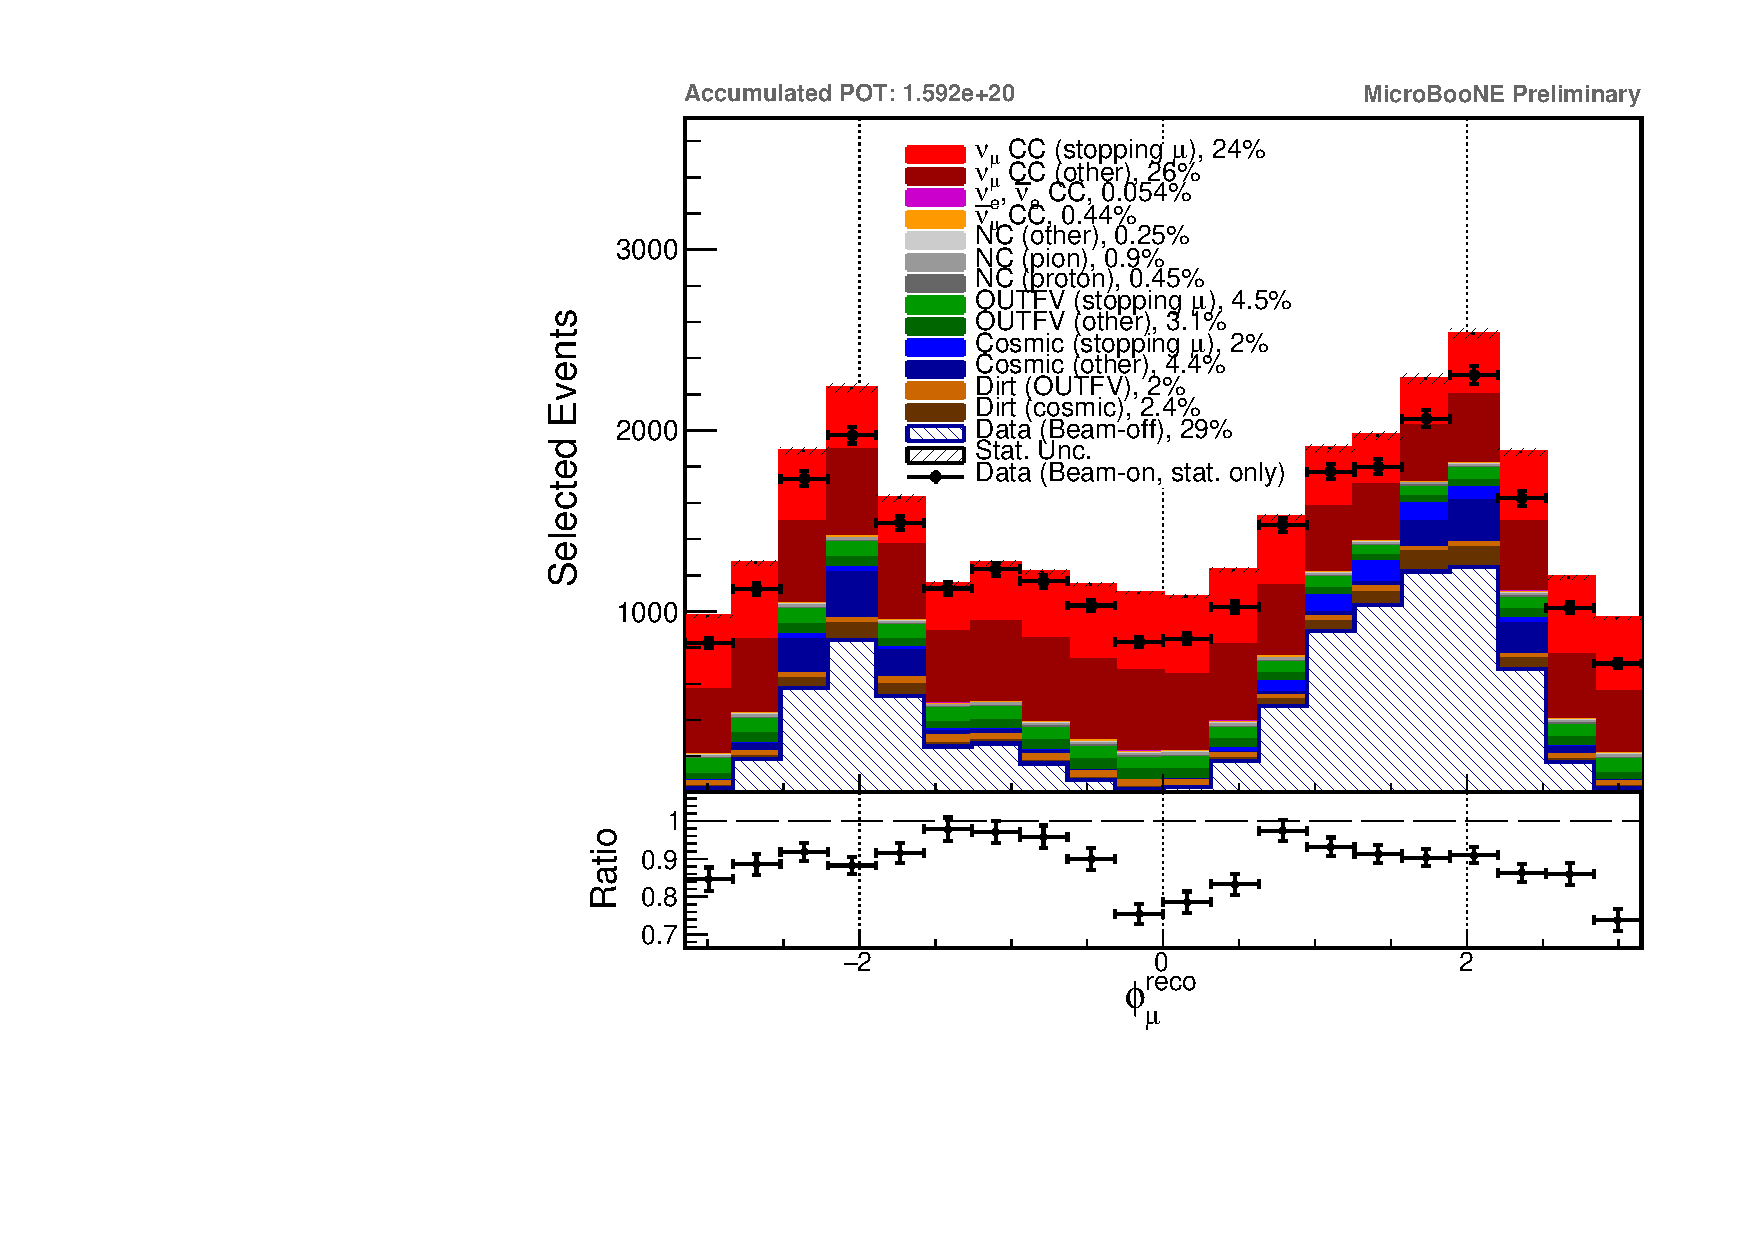
\includegraphics[width=.45\textwidth]{images/DataMC_Tune1/trkphi_tune1}
   \label{fig:trkphi_tune1}} \quad
\subfloat[][\tunethree.]
   {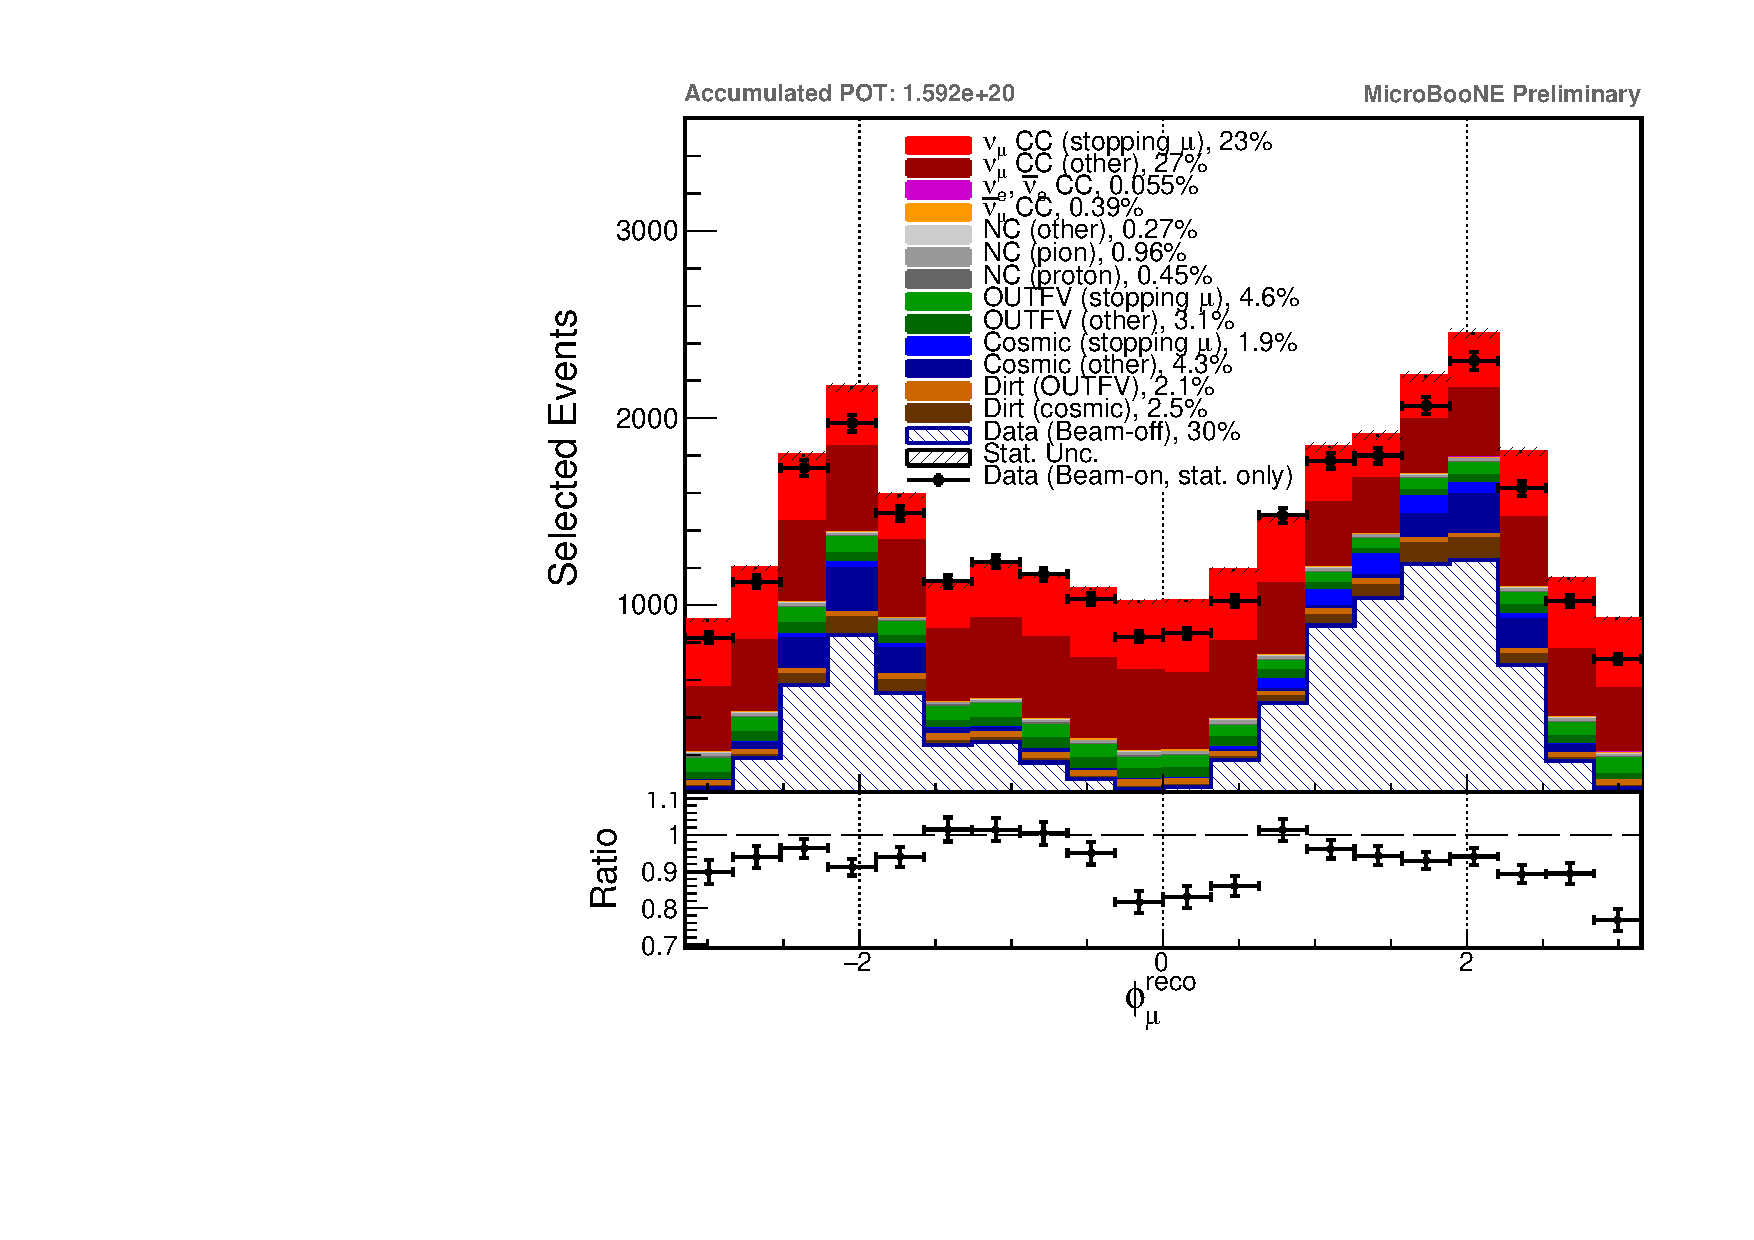
\includegraphics[width=.45\textwidth]{images/DataMC_Tune3/trkphi_tune3}
   \label{fig:trkphi_tune3}} \quad
\subfloat[][\tuneone.]
   {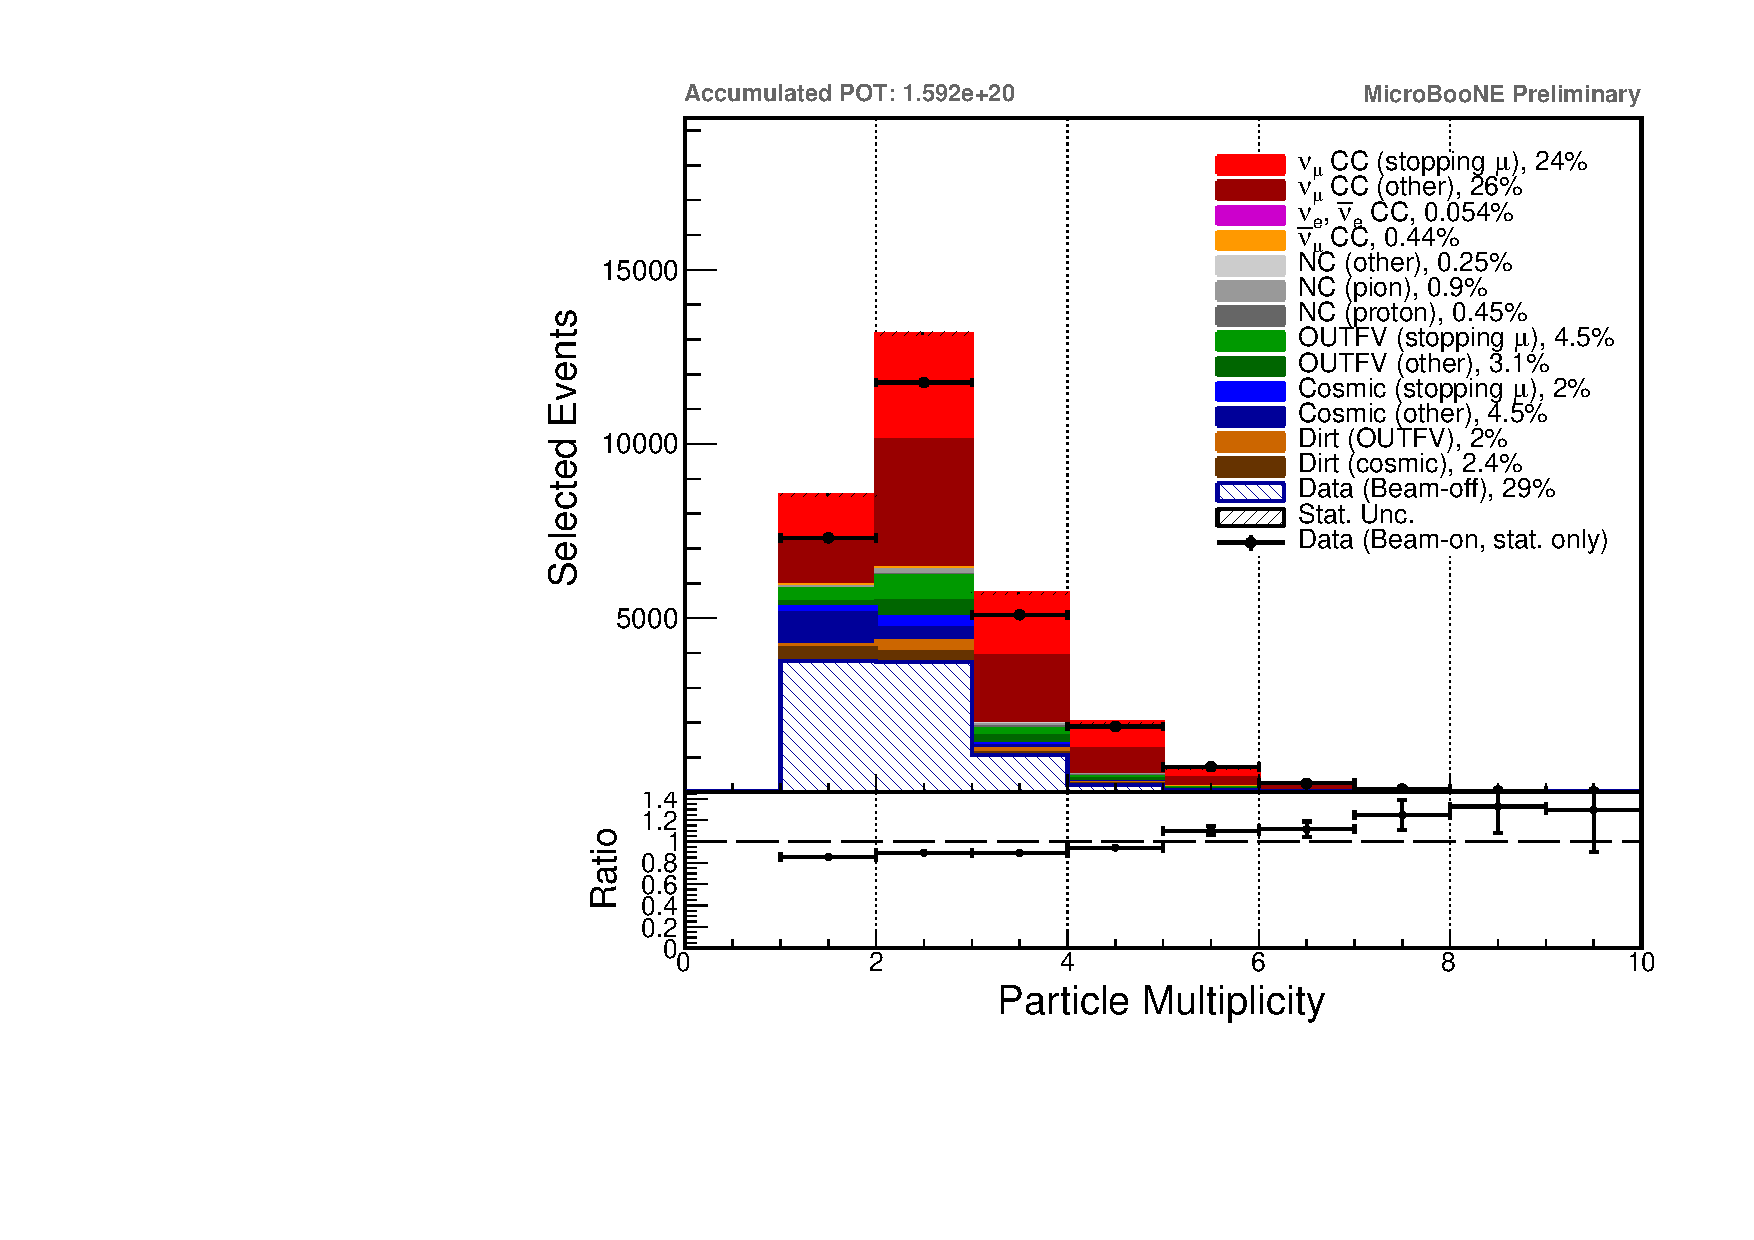
\includegraphics[width=.45\textwidth]{images/DataMC_Tune1/multpfp_tune1}
   \label{fig:multpfp_tune1}} \quad
\subfloat[][\tunethree.]
   {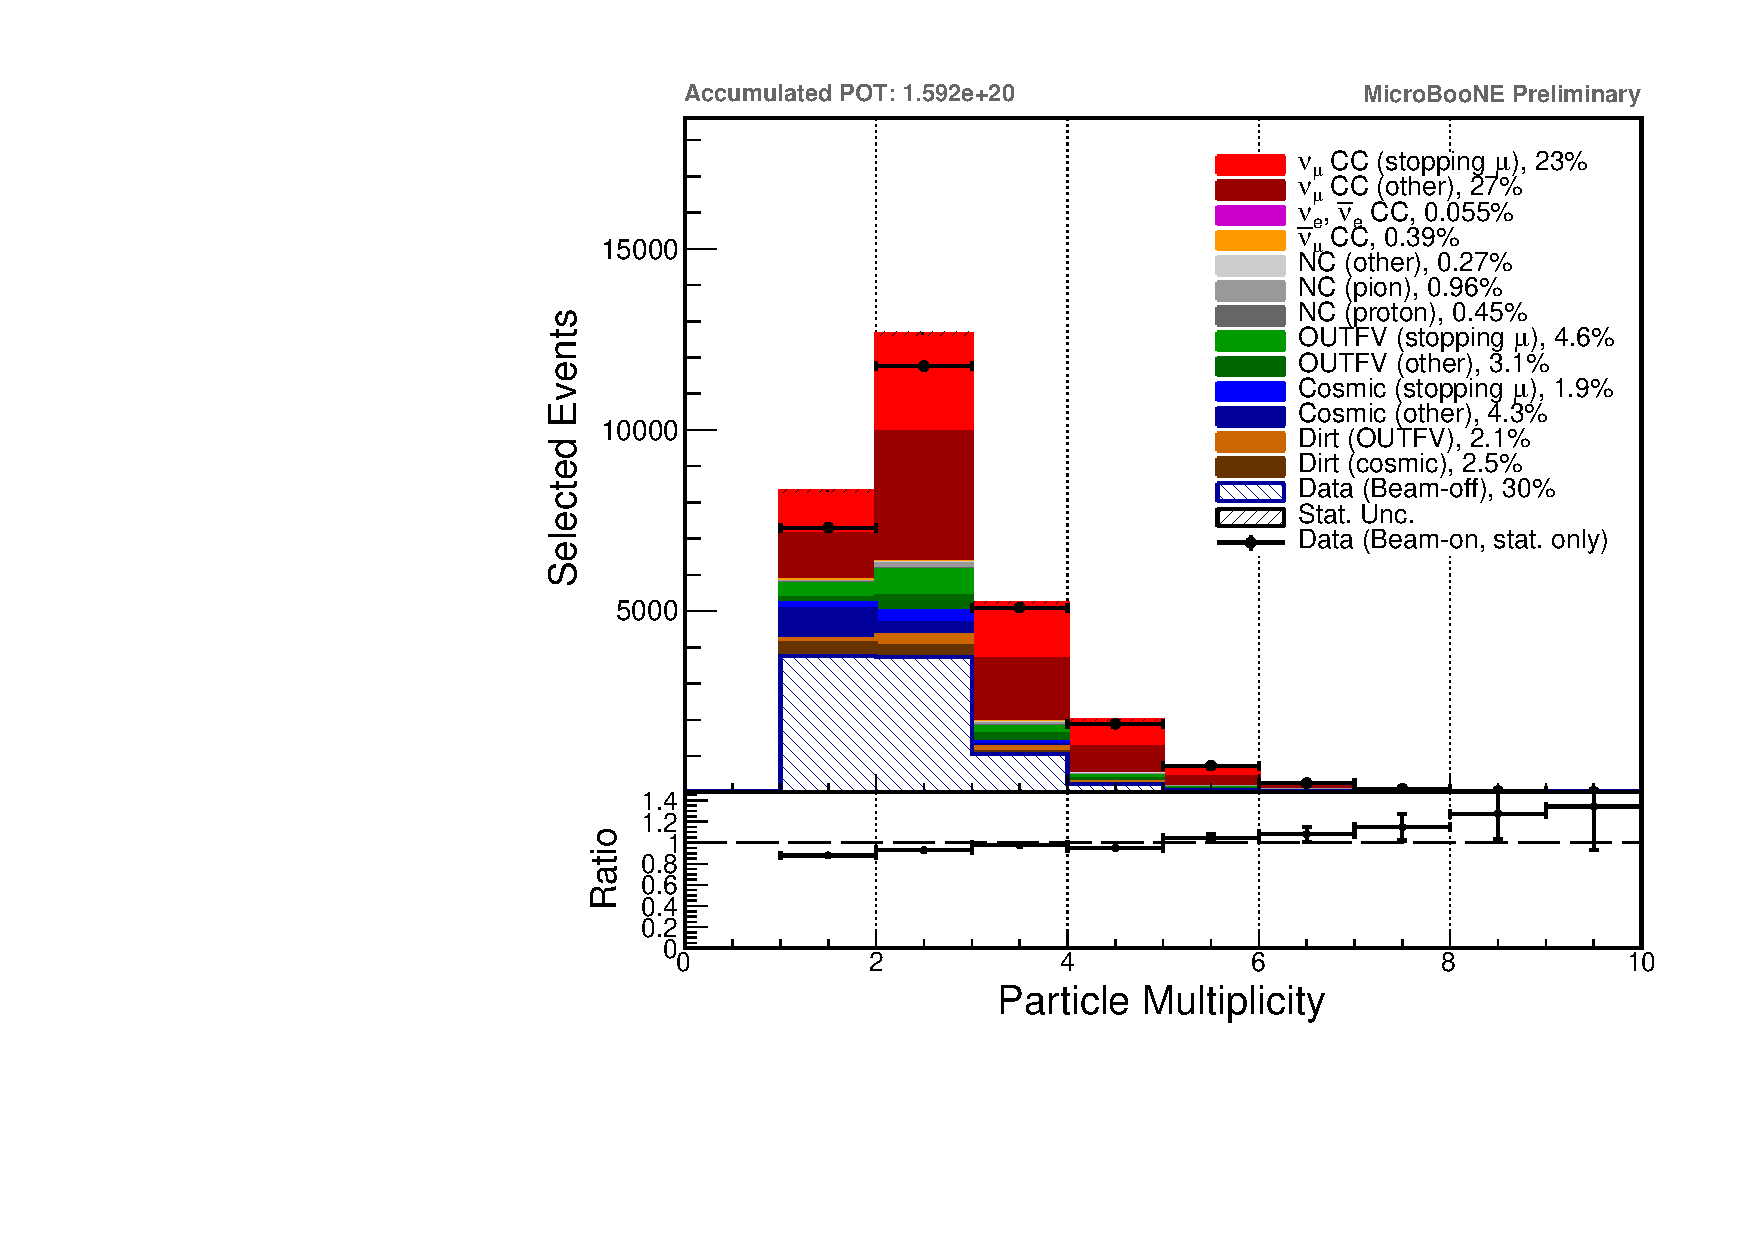
\includegraphics[width=.45\textwidth]{images/DataMC_Tune3/multpfp_tune3}
   \label{fig:multpfp_tune3}} \quad
%\subfloat[][\tuneone.]
%   {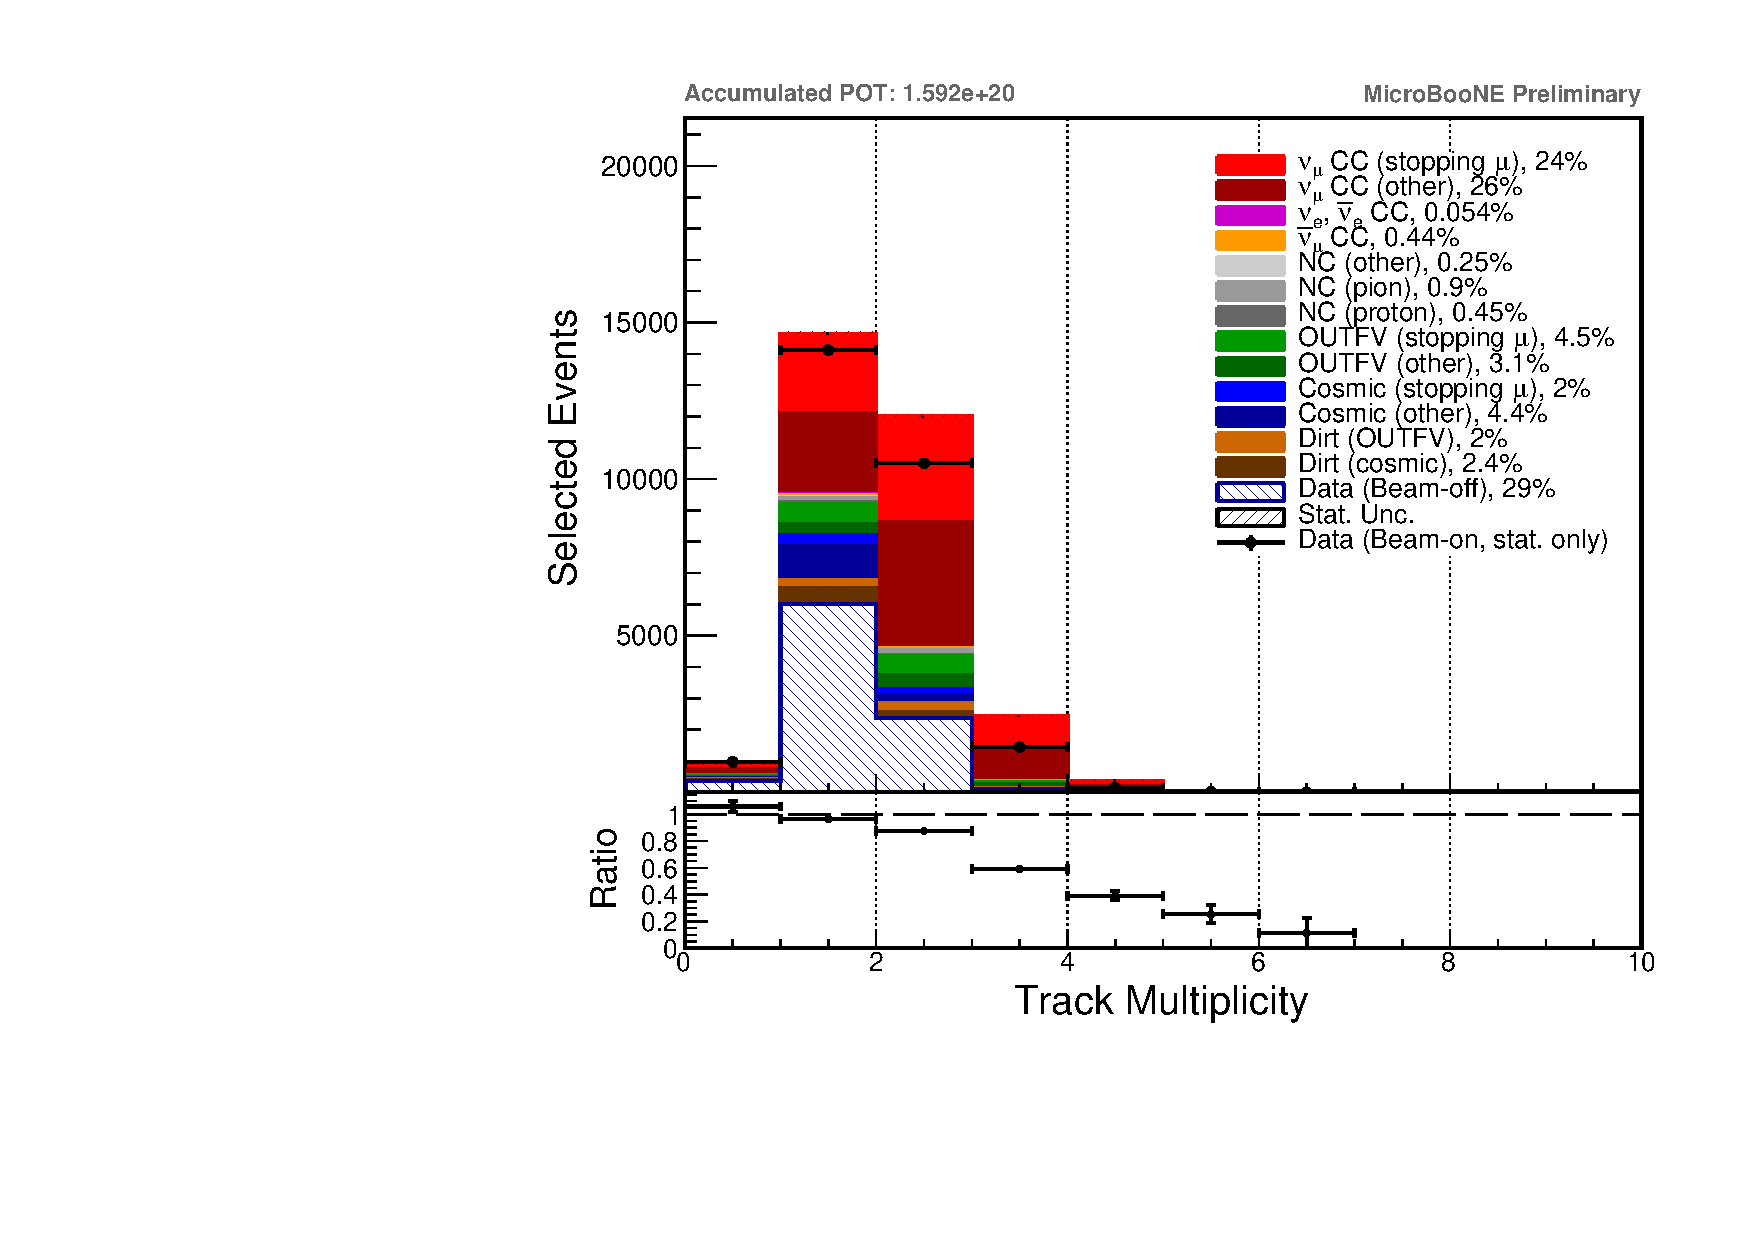
\includegraphics[width=.45\textwidth]{images/DataMC_Tune1/multtracktol_tune1}
%   \label{fig:multtracktol_tune1}} \quad
%\subfloat[][\tunethree.]
%   {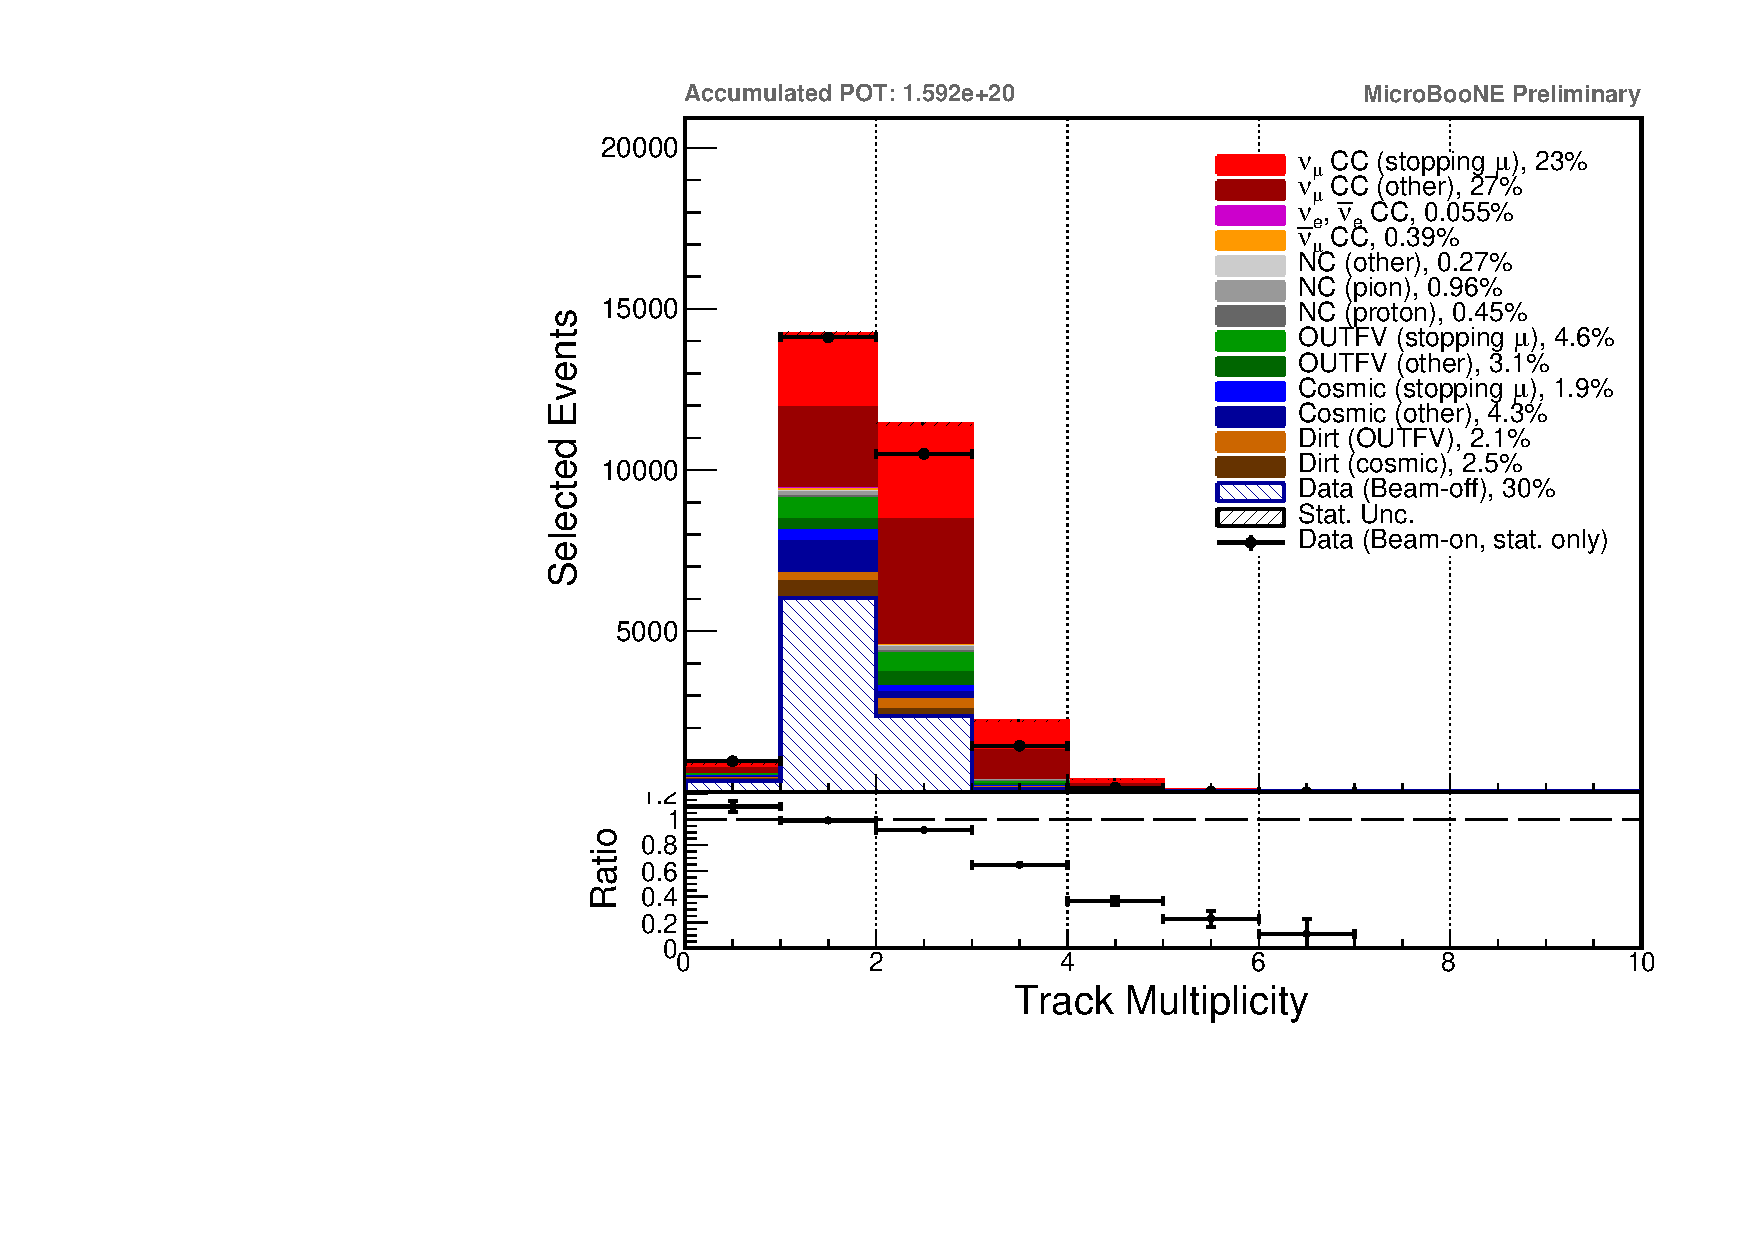
\includegraphics[width=.45\textwidth]{images/DataMC_Tune3/multtracktol_tune3}
%   \label{fig:multtracktol_tune3}} \quad
\caption[Distribution of Selected Events ($\phi$, multiplicity)]{\emph{(continues)} Event distributions of the selected events. The black data points symbolise beam-on data with statistical uncertainties. The stacked coloured histograms represent the simulation, with the shaded bands representing the statistical uncertainty only. The red histograms shows the signal events. The hashed histogram is beam-off data. Data and \acrshort{mc} correspond to $1.592 \times 10^{20}$ \acrshort{pot}. Left plots show \acrshort{mc} from the ``\tuneone'' configuration, right ones from the ``\tunethree'' configuration.}
\label{fig:final_dist}
\end{figure}
%
\begin{figure}[]
\ContinuedFloat
\centering
\subfloat[][\tuneone.]
   {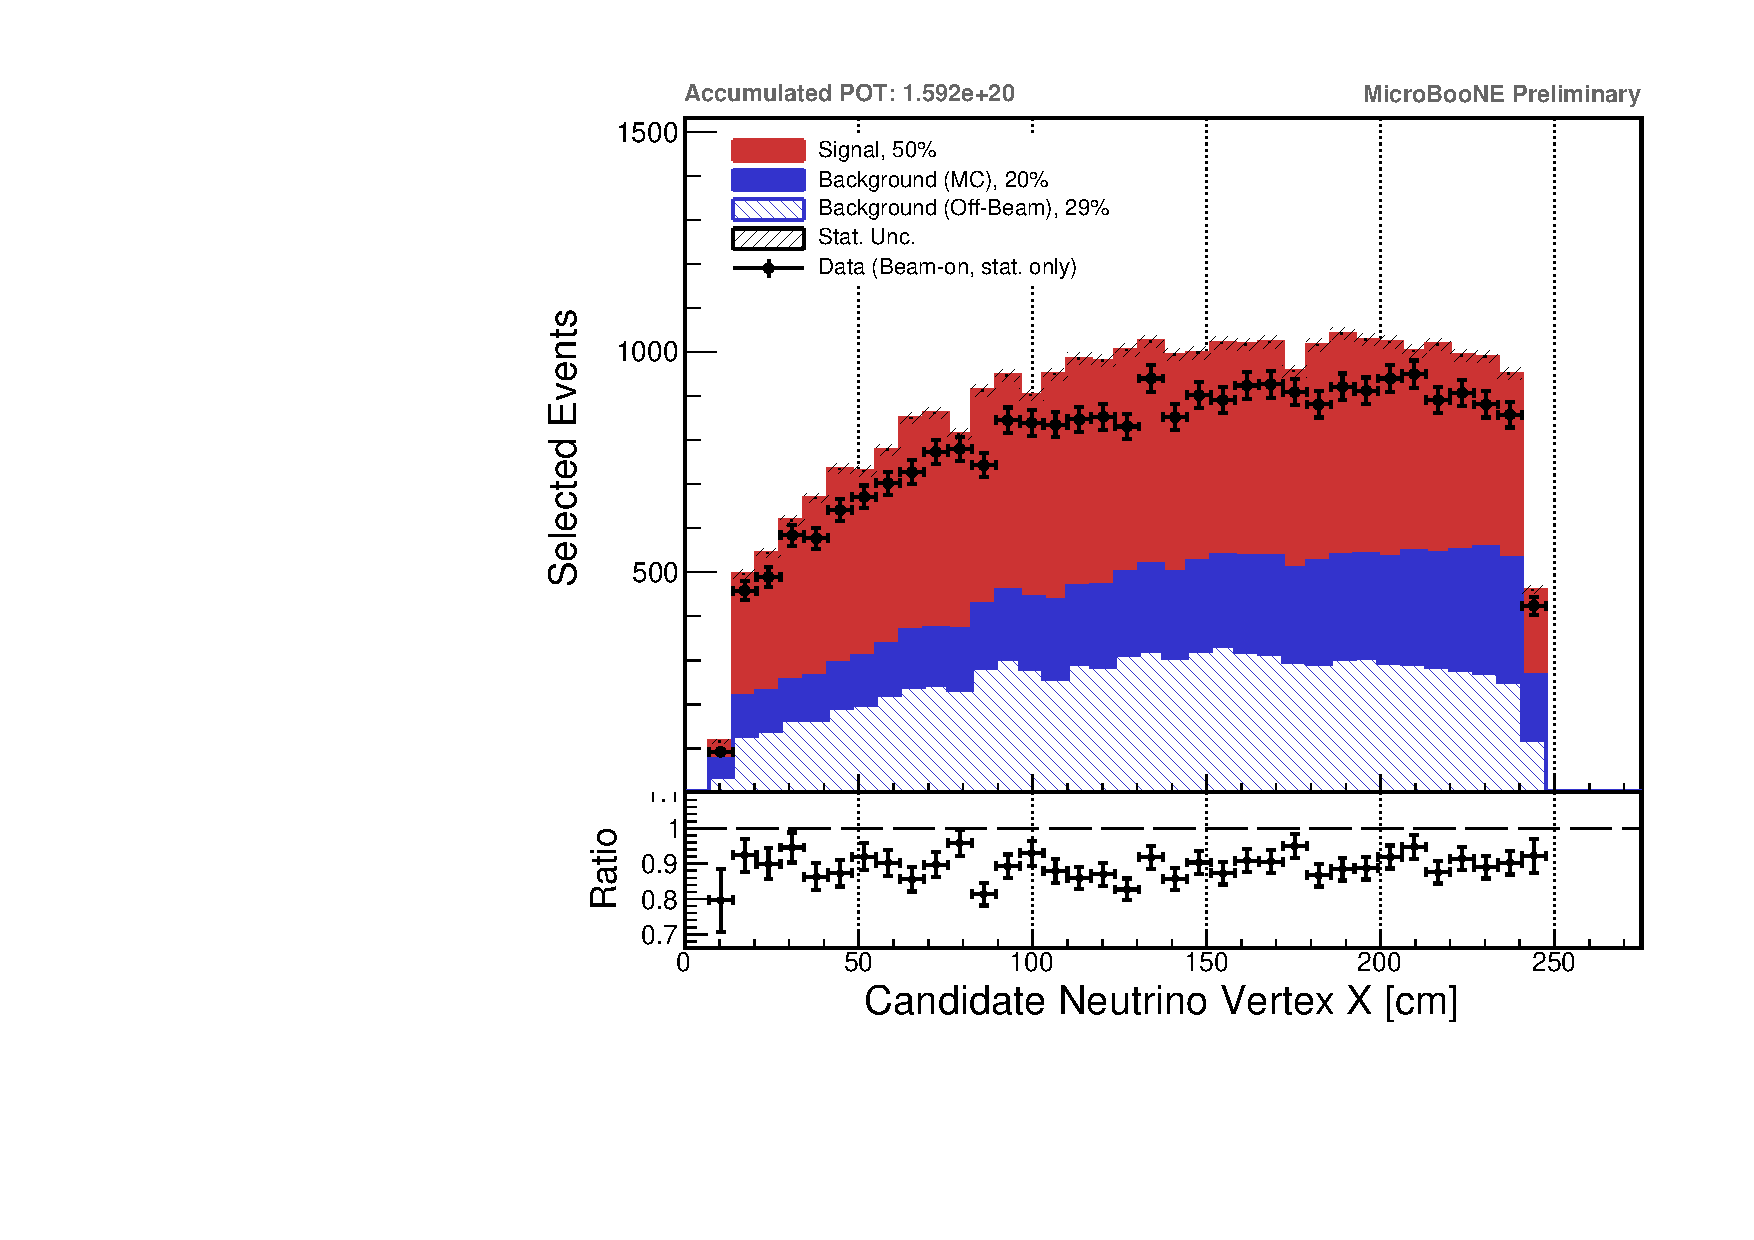
\includegraphics[width=.45\textwidth]{images/DataMC_Tune1/vtxx_tune1}
   \label{fig:vtxx_tune1}} \quad
\subfloat[][\tunethree.]
   {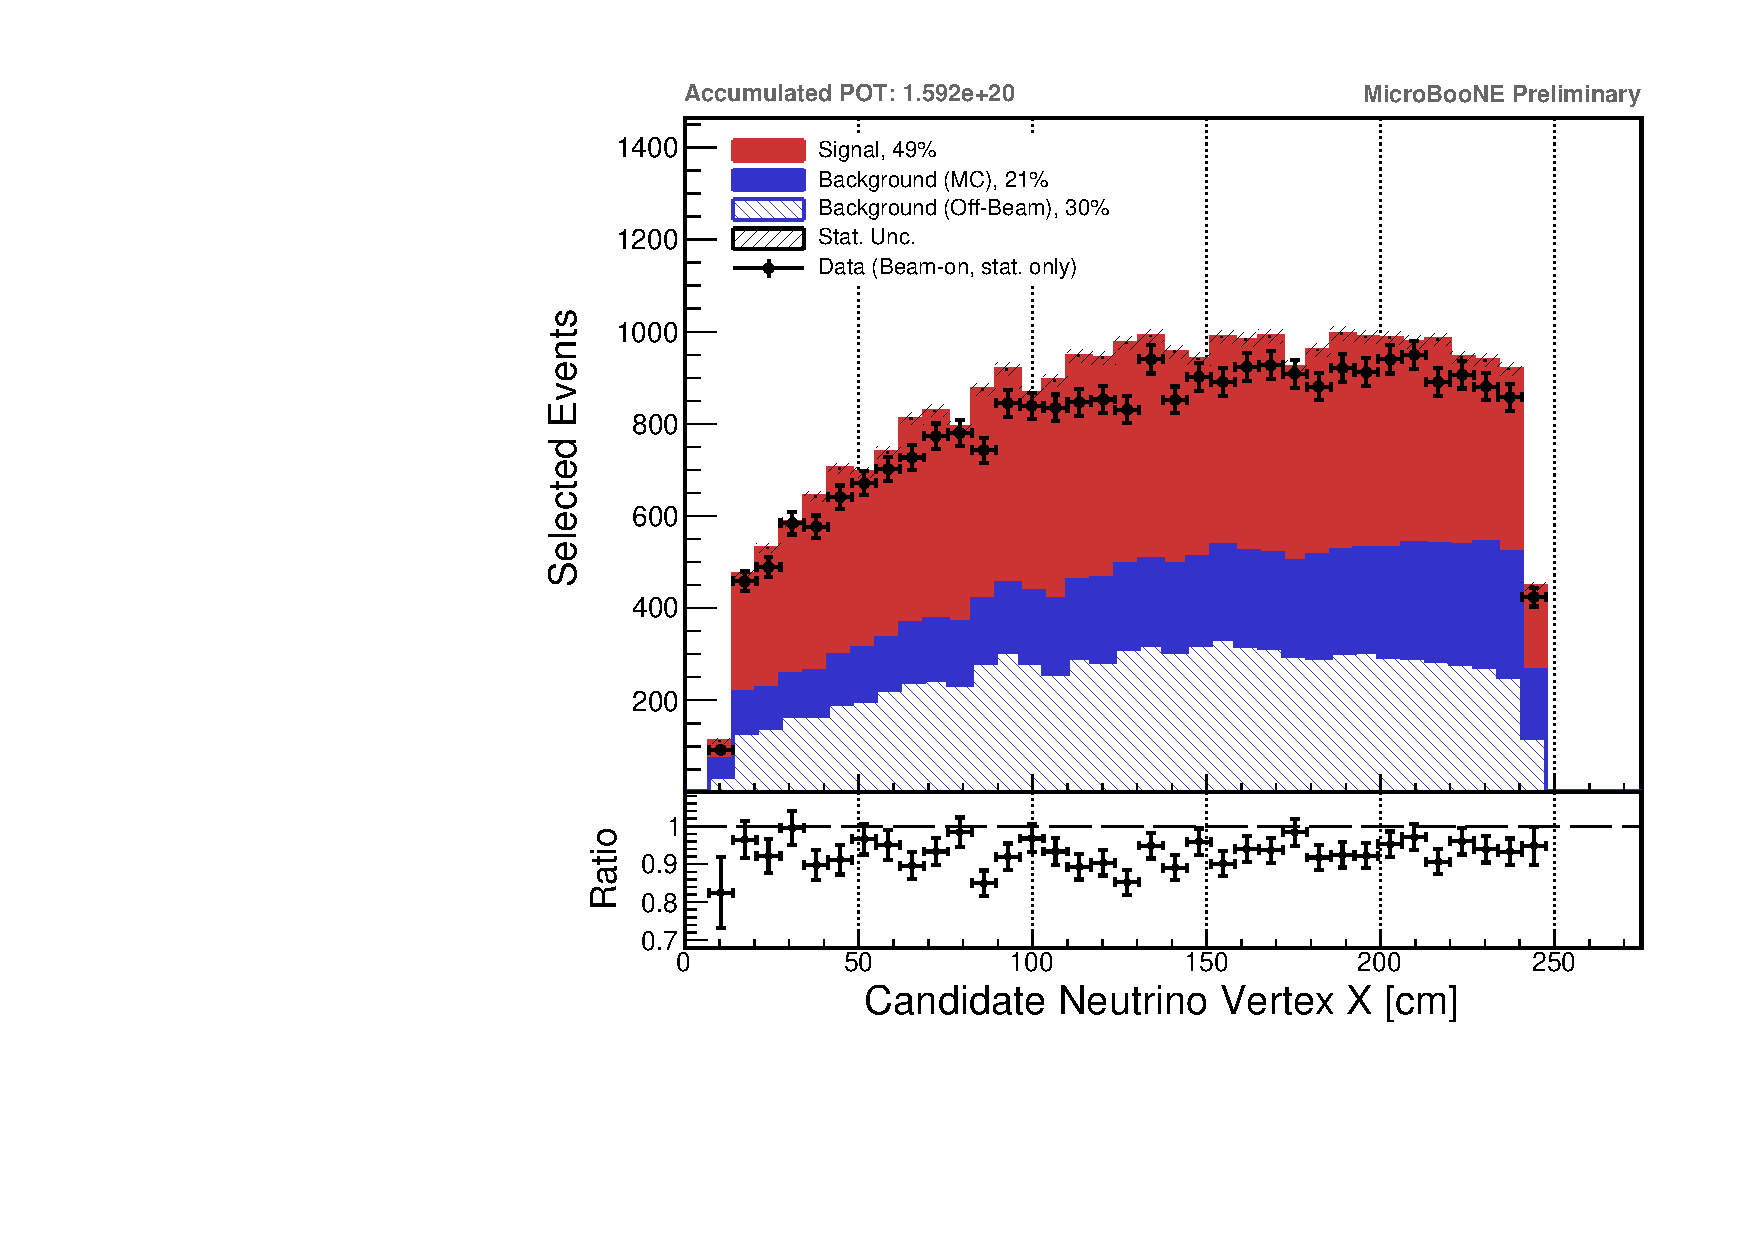
\includegraphics[width=.45\textwidth]{images/DataMC_Tune3/vtxx_tune3}
   \label{fig:vtxx_tune3}} \quad
\subfloat[][\tuneone.]
   {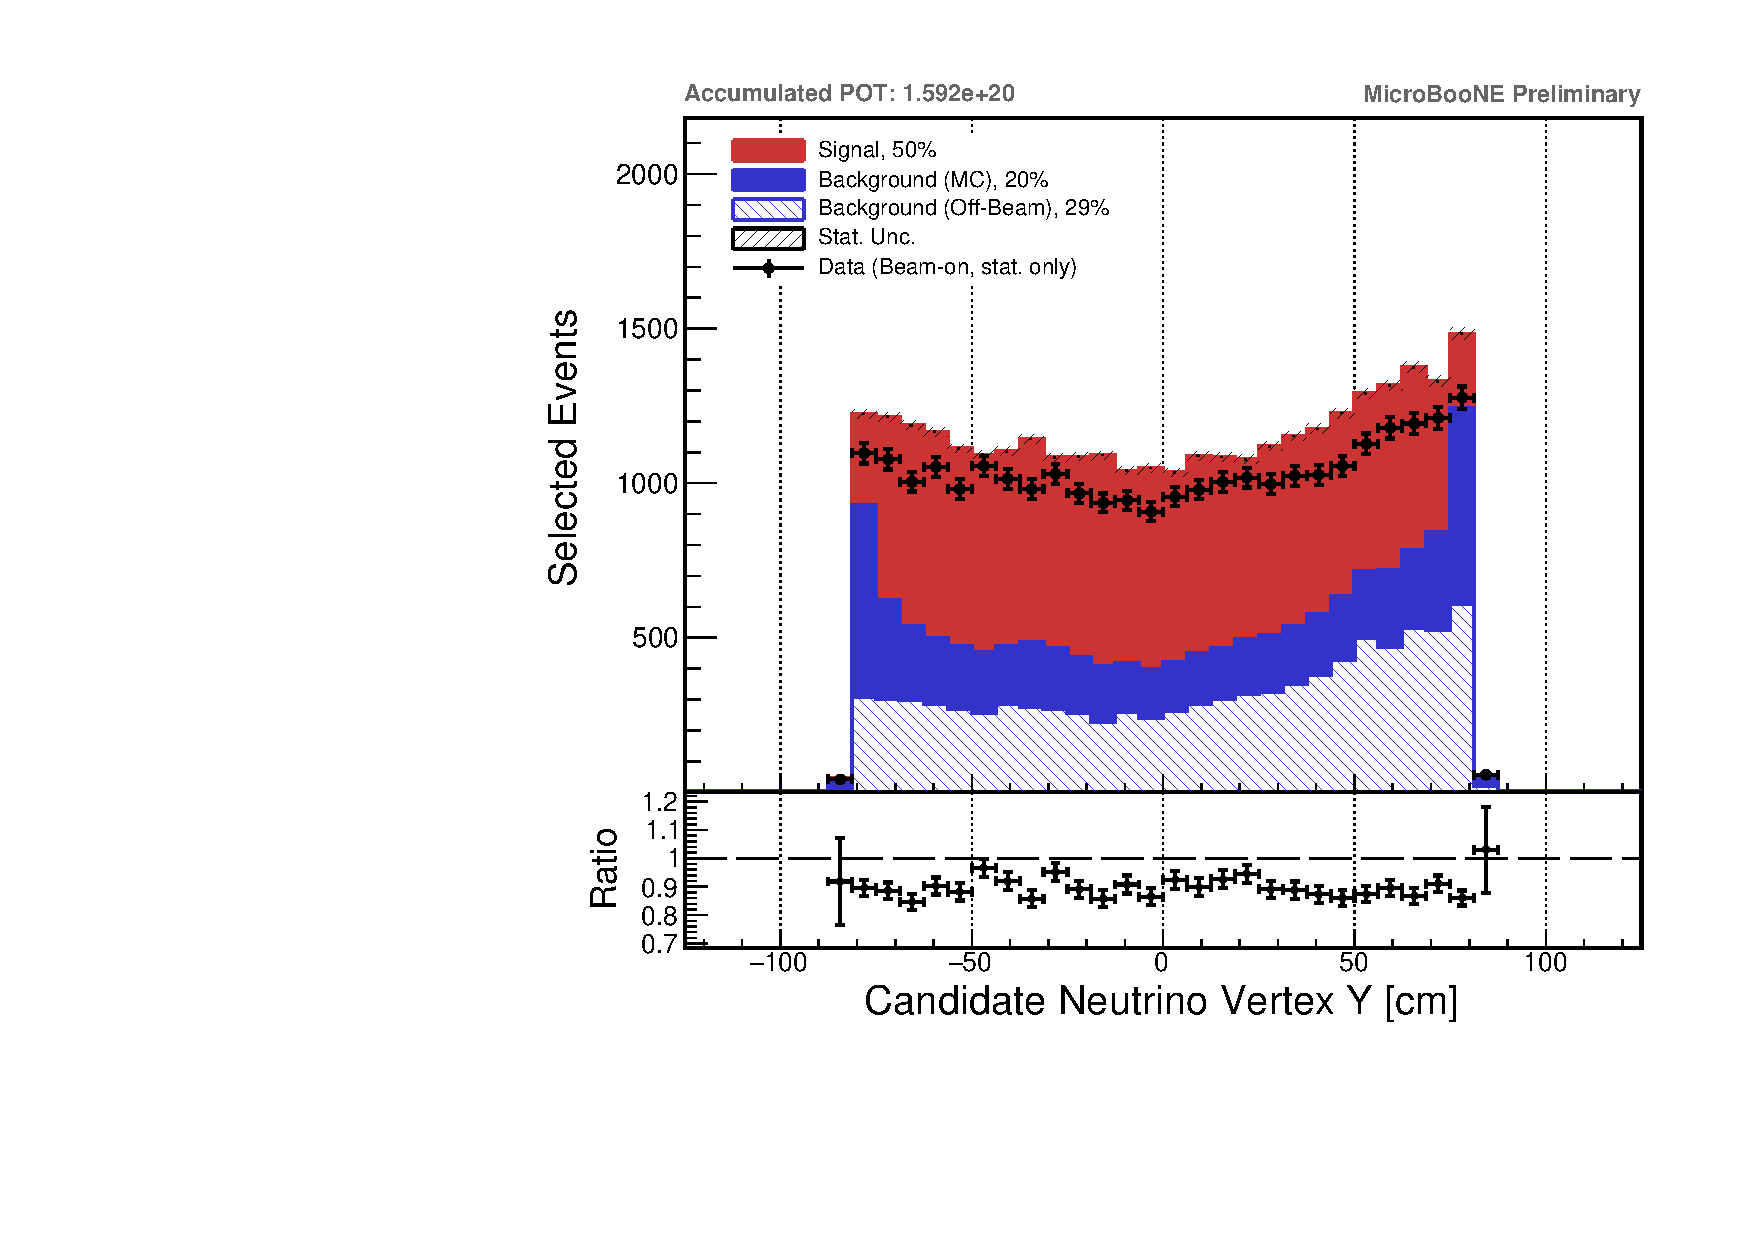
\includegraphics[width=.45\textwidth]{images/DataMC_Tune1/vtxy_tune1}
   \label{fig:vtxy_tune1}} \quad
\subfloat[][\tunethree.]
   {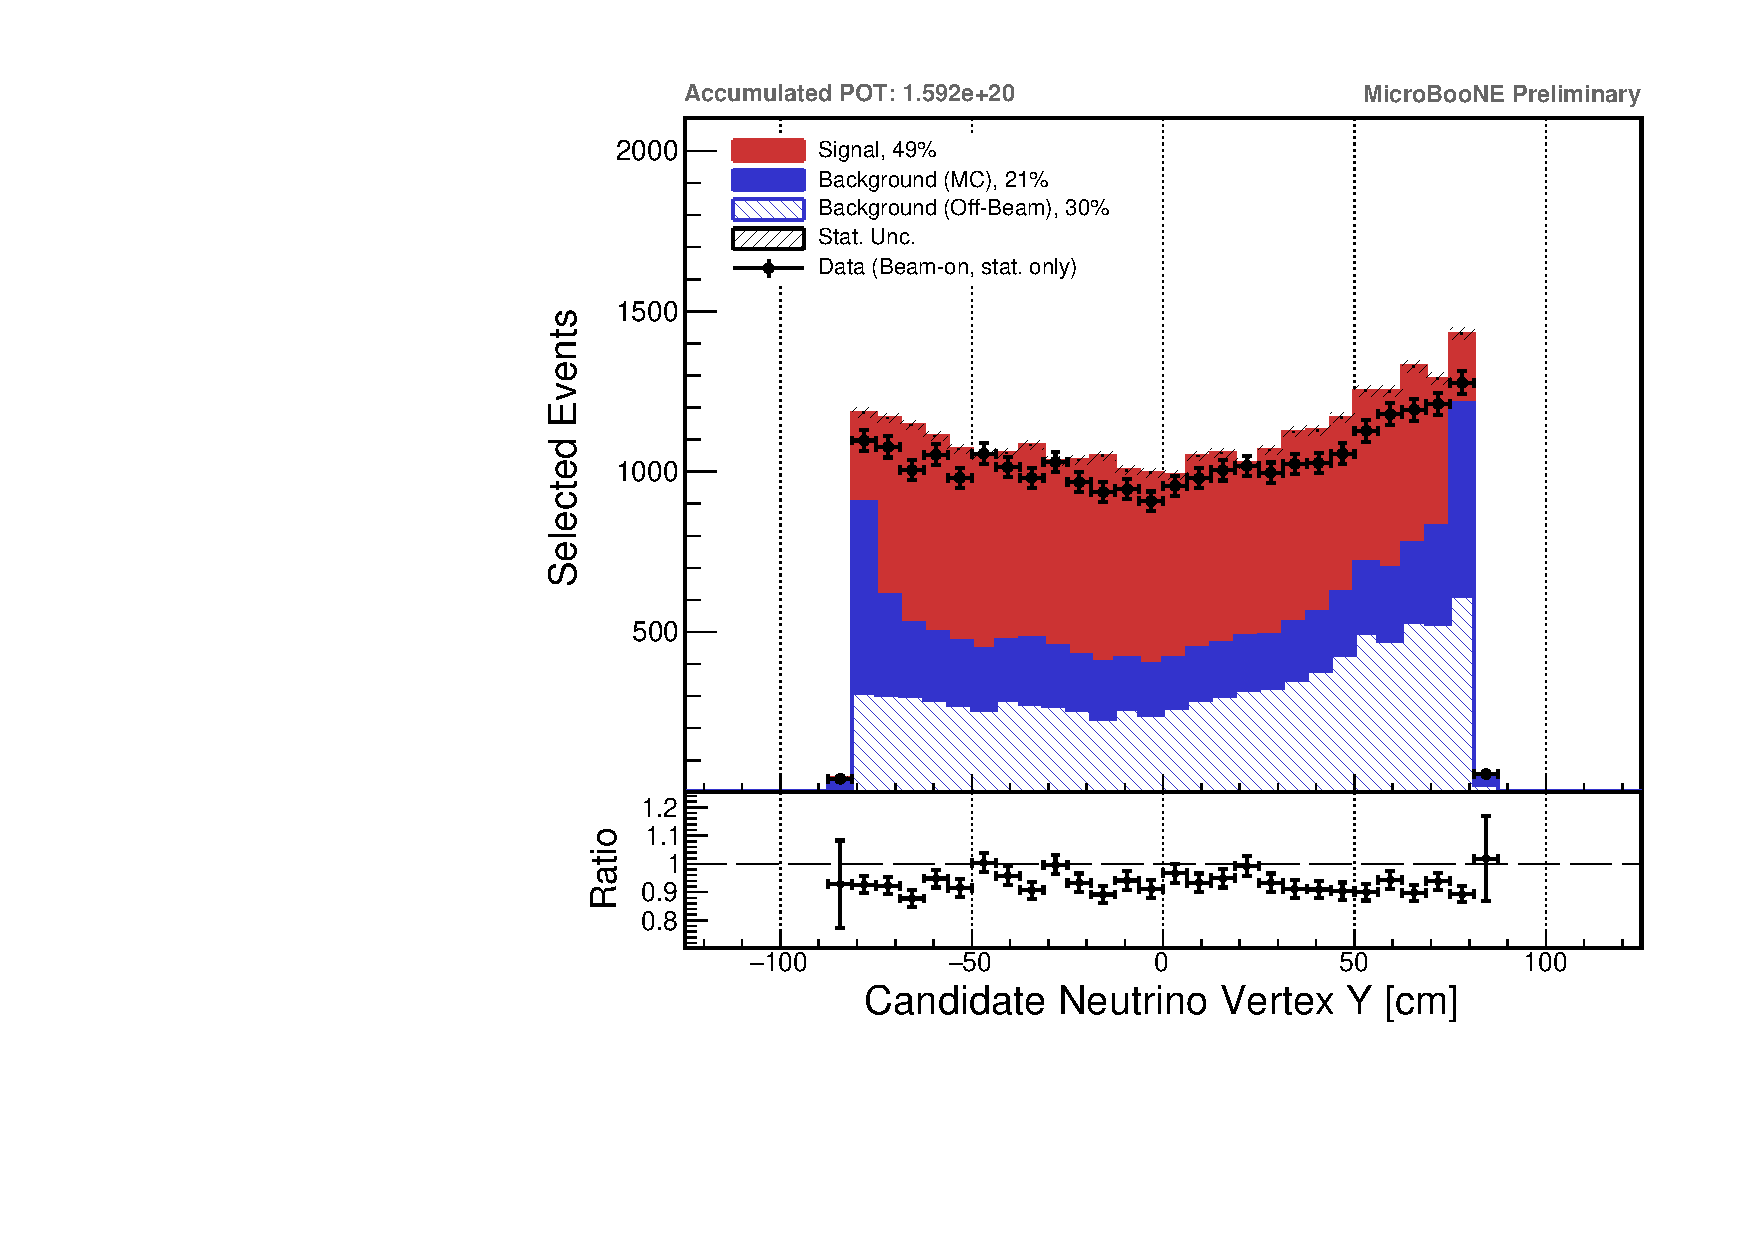
\includegraphics[width=.45\textwidth]{images/DataMC_Tune3/vtxy_tune3}
   \label{fig:vtxy_tune3}} \quad
\subfloat[][\tuneone.]
   {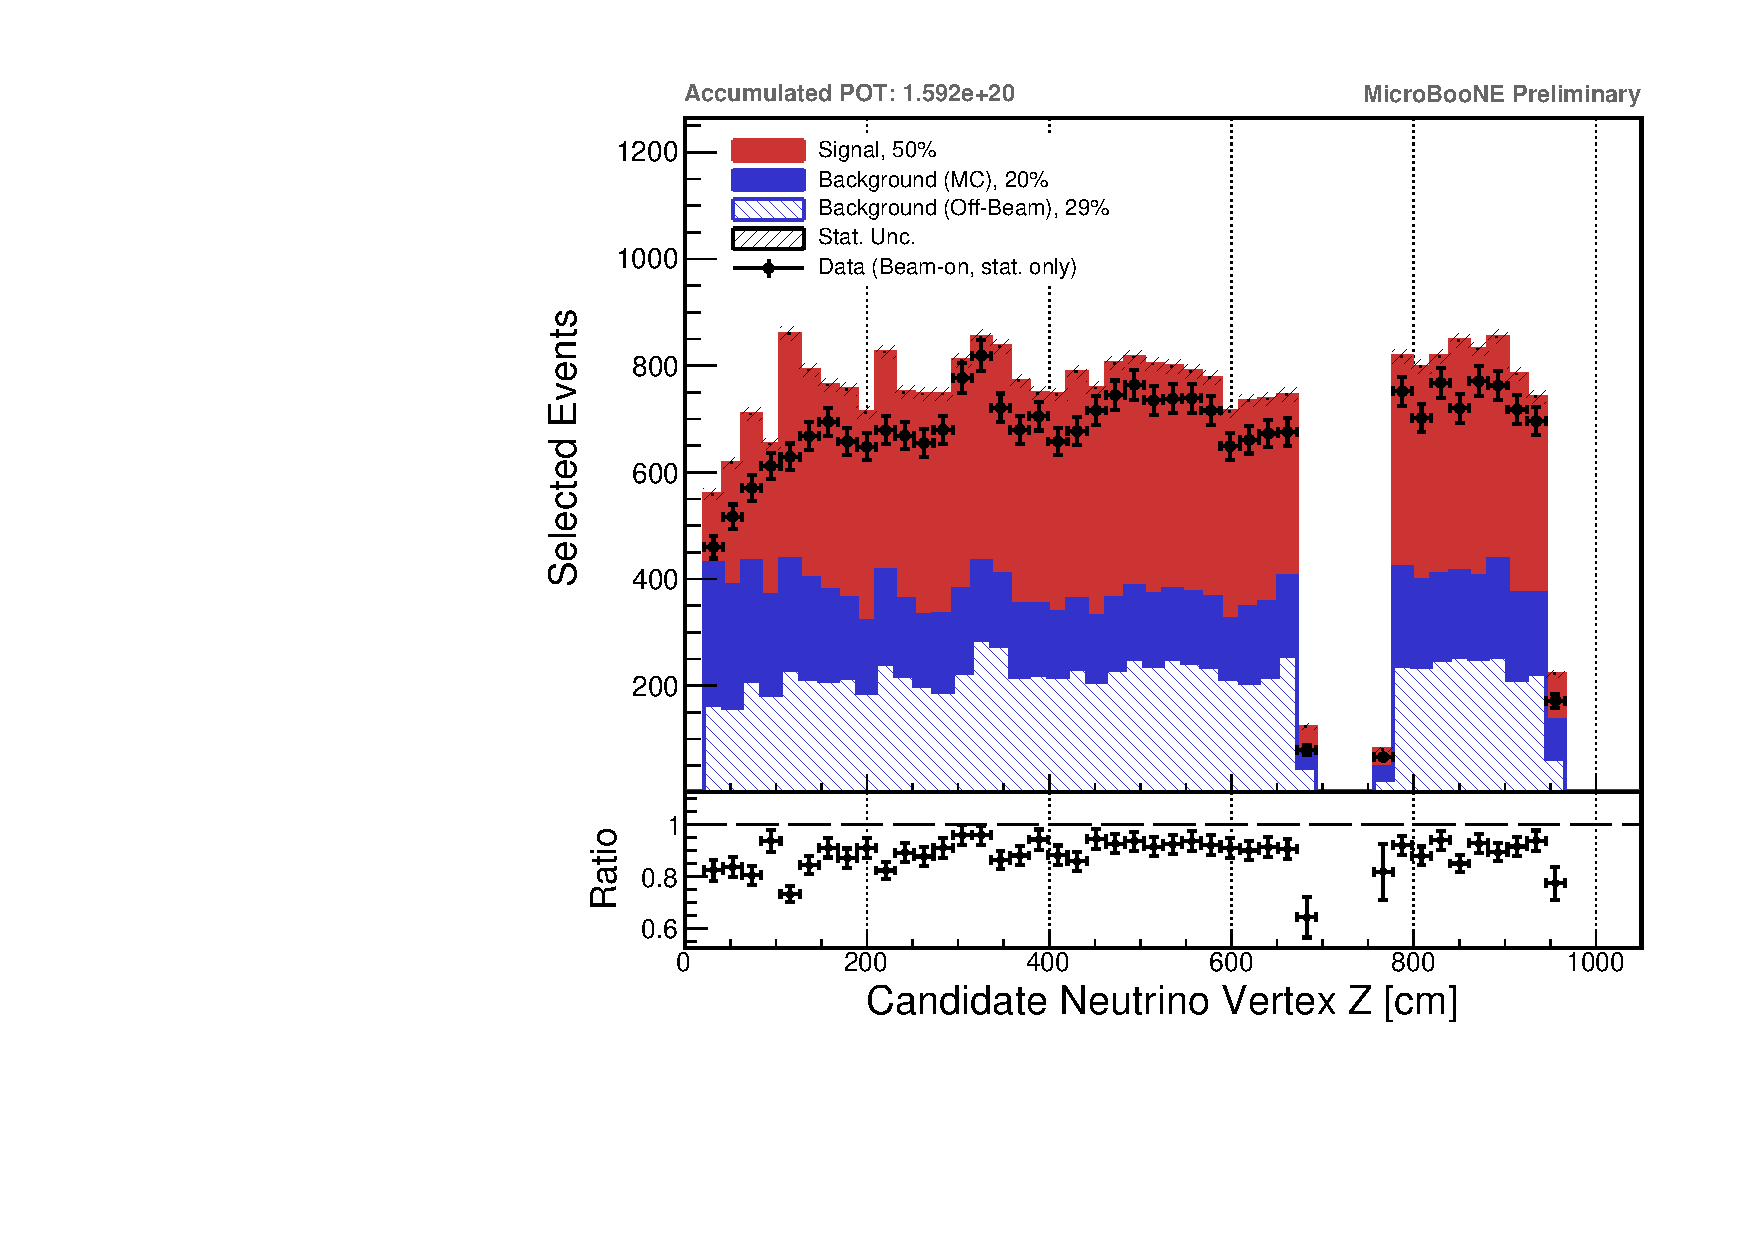
\includegraphics[width=.45\textwidth]{images/DataMC_Tune1/vtxz_tune1}
   \label{fig:vtxz_tune1}} \quad
\subfloat[][\tunethree.]
   {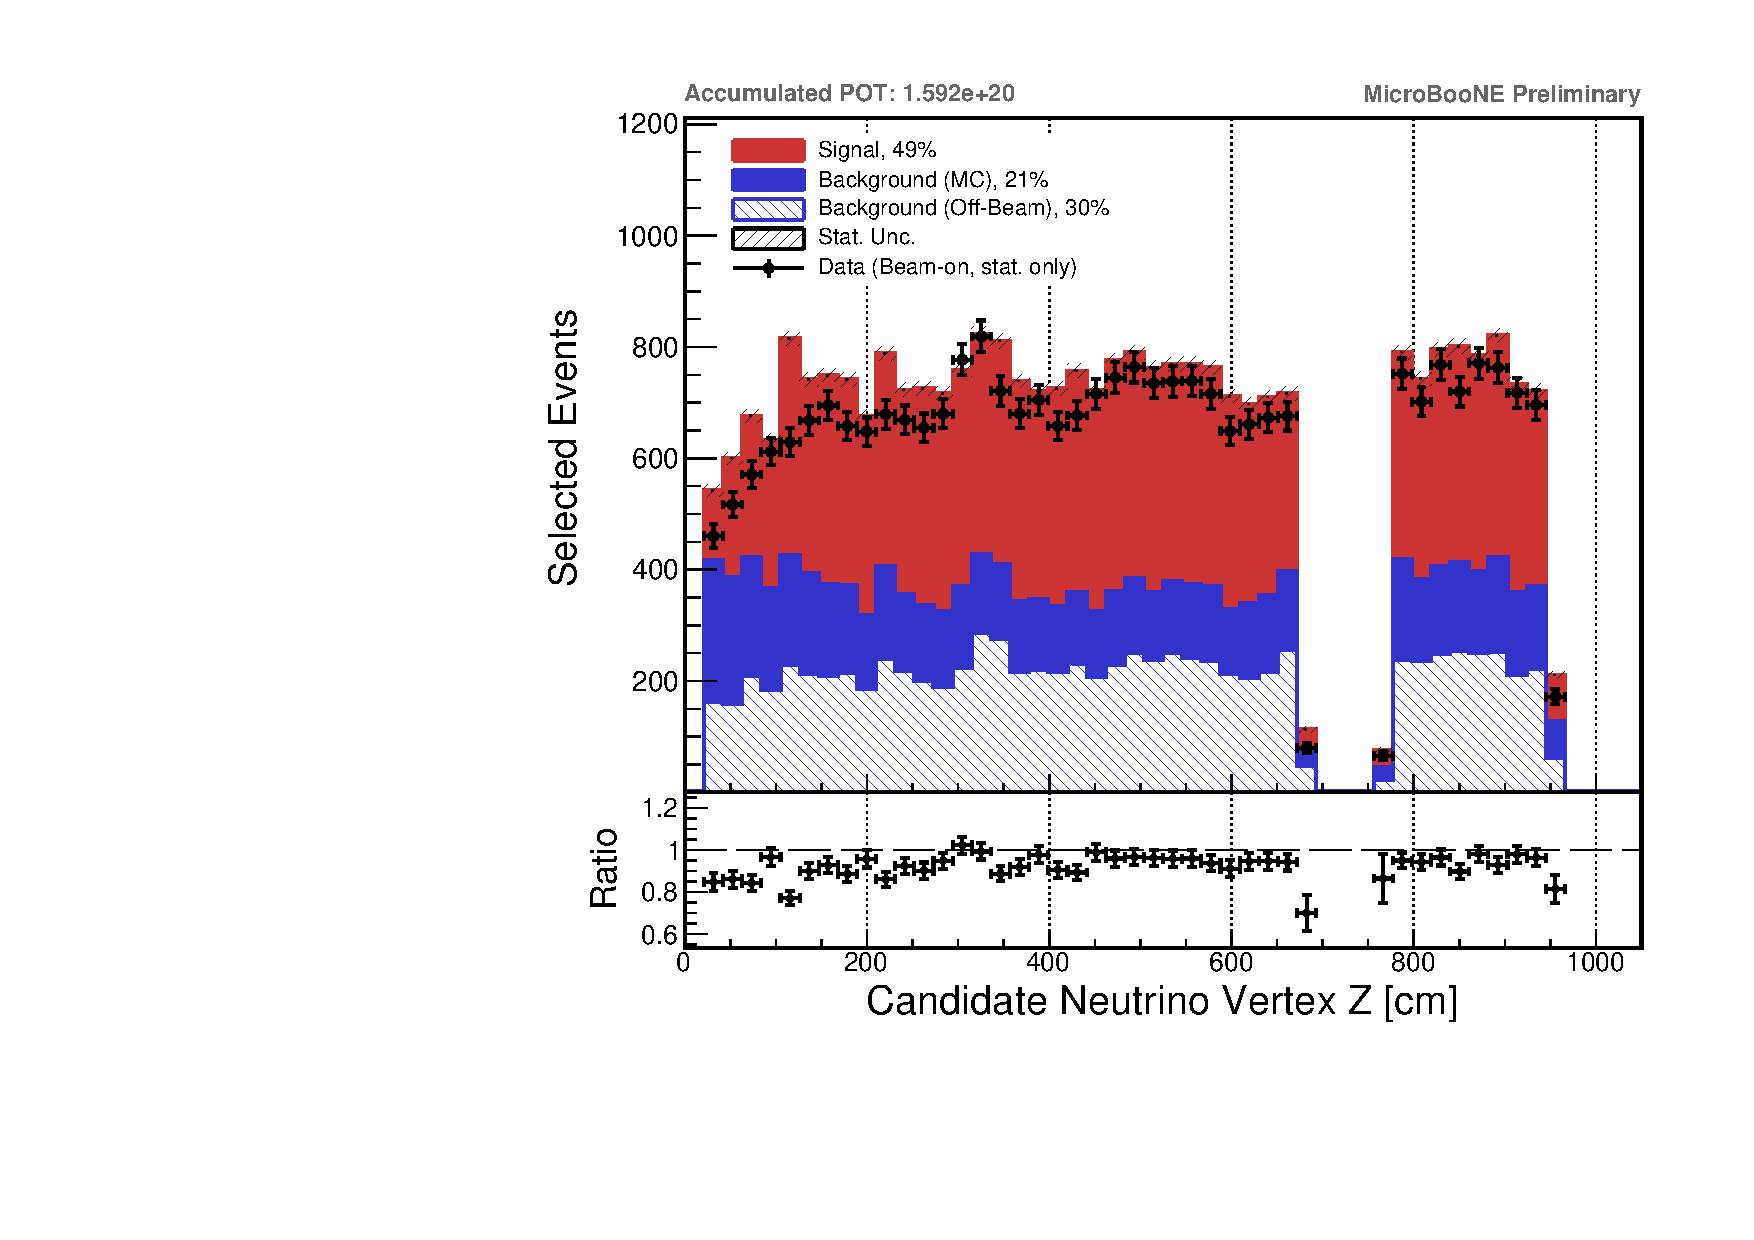
\includegraphics[width=.45\textwidth]{images/DataMC_Tune3/vtxz_tune3}
   \label{fig:vtxz_tune3}} \quad
\caption[Distribution of Selected Events (Vertex $x$, $y$ and $z$)]{\emph{(continues)} Event distributions of the selected events. The black data points symbolise beam-on data with statistical uncertainties. The stacked coloured histograms represent the simulation, with the shaded bands representing the statistical uncertainty only. The red histograms shows the signal events. The hashed histogram is beam-off data. Data and \acrshort{mc} correspond to $1.592 \times 10^{20}$ \acrshort{pot}. Left plots show \acrshort{mc} from the ``\tuneone'' configuration, right ones from the ``\tunethree'' configuration.}
\label{fig:final_dist}
\end{figure}
%
\begin{figure}[]
\centering
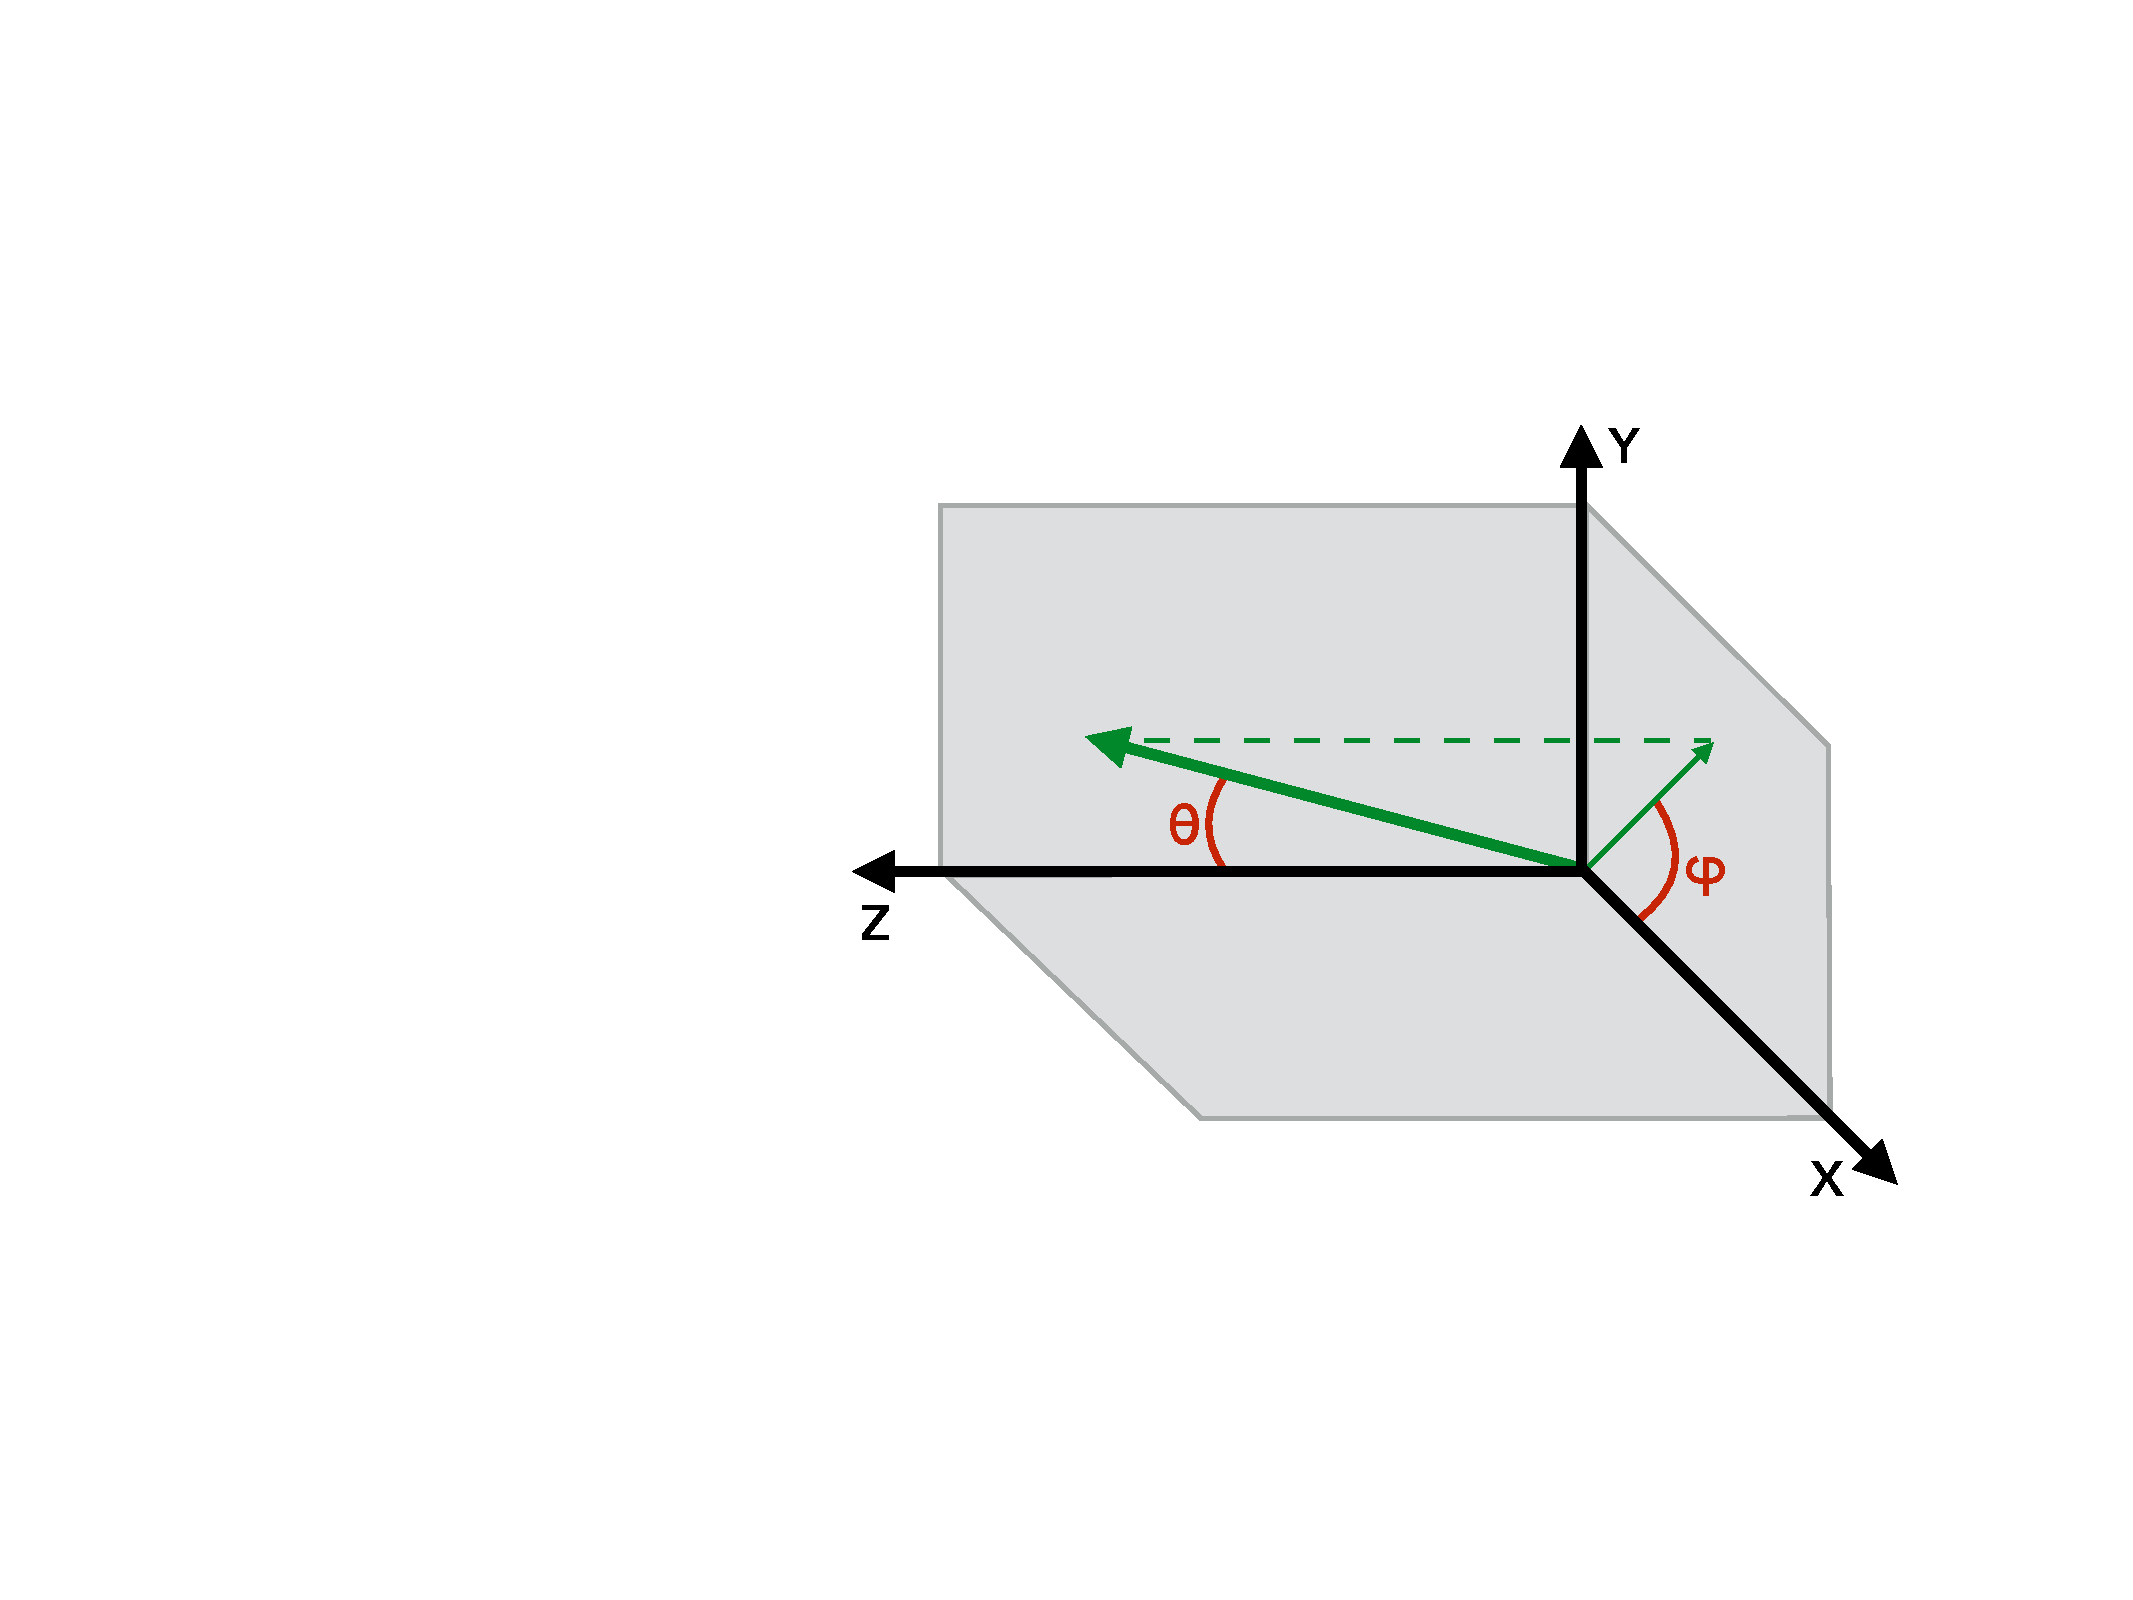
\includegraphics[width=.45\textwidth]{images/coord_system}
\caption[MicroBooNE Coordinate System]{MicroBooNE coordinate system showing the definition of the polar angle $\theta$ and the azimuthal angle $\phi$ for a given track (green). The neutrino beam runs along the $z$ axis. The anode is at $x = 0$.}
\label{fig:coord_system}
\end{figure}
%
The stacked coloured histograms in Figure~\ref{fig:final_dist} represent the \acrshort{mc} simulation for signal events in red and for all the estimated backgrounds. The \acrshort{mc} is normalised to the same \acrshort{pot} as the data. The different backgrounds are:
\begin{description}
\item[Cosmic Rays] Events where a neutrino interaction is present (usually producing optical activity in the beam window), but a \acrshort{cr} interaction is selected instead. Some \acrshort{cr}s will enter the \acrshort{tpc} from regions of the detector with unresponsive wires, with the result that the beginning of the track is not reconstructed. This \acrshort{cr}s may look as spatially contained tracks. 
\item[Neutrinos Interacting Outside the Fiducial Volume (\acrshort{outfv})] Events where the neutrino interacts outside the fiducial volume, but produces a muon that crosses (or stops in) the \acrshort{tpc}, that is then selected. In these events the vertex is mis-reconstructed and appears to be in the \acrshort{fv}, leading to wrong momentum and angle reconstruction. 
%These events are not signal events as the true neutrino interaction vertex is outside the \acrshort{fv}.
\item[Dirt] Events coming from the ``dirt'' simulated sample. They are due to interactions that happen outside the cryostat. The ``dirt'' contributes to two backgrounds: a \acrshort{cr} background (usually because there is a neutrino induced flash, but a \acrshort{cr} is selected instead) and an \acrshort{outfv} background (in which a neutrino origin track is selected).
\item[(Anti-)Electron Neutrinos] Events where an electron from a $\nu_e$ or a $\bar{\nu}_e$ interaction is selected. $\nu_e$ and $\bar{\nu}_e$ are a small contamination in the \acrshort{bnb} beam. This usually happens because the electron is reconstructed as a track instead of an electromagnetic shower.
\item[Anti-Muon Neutrinos] Events where a muon from a $\bar{\nu}_\mu$ interaction is selected. $\bar{\nu}_\mu$ are a small contamination in the \acrshort{bnb} beam. MicroBooNE is not provided with a magnetic field that help to distinguish a $\bar{\nu}_\mu$ from a $\nu_\mu$ by the curvature of the $\mu^+$ or $\mu^-$ in the final state.
\item[Neutral Current] Events where a neutral current event is selected, usually a pion in the final state is selected as muon candidate.
\end{description}
Table \ref{tab:background_perc} shows the background contamination percentages, indicating that the main background is from \acrshort{cr}s, followed by \acrshort{outfv} interactions. 
%The distributions with all backgrounds (beam-off and \acrshort{mc}) subtracted used for the double differential cross section will be shown in the next Chapter.
Some relevant features in the distributions shown in Figure~\ref{fig:final_dist} are discussed in the next points:
\begin{itemize}
%\item There is a bump in the backward region, as it can be seen in the $\cos\theta$ distribution. This has been investigated and some studies have been shown in \cite{backward_bump}. We are pretty confident that that bump is beam induced, created by neutrinos that interact in the dirt and enter the detector from upstream. They then stop in the TPC and are reconstructed as going backward. We have tried to remove them by looking at the MCS fit results in both directions, but this is not sufficient to remove all of them (plus it reduces the selection efficiency). A request has been made to produce a dirt sample to confirm this. The production should start soon (05-02-18).
\item The $\cos\theta_\mu$ distribution in \subref{fig:trkcostheta_tune1} and \subref{fig:trkcostheta_tune3} shows a bump around $\cos\theta_\mu = 0$. This is caused by \acrshort{cr} background. The distribution for \acrshort{cr} should be symmetric, but Pandora reconstruction has a bias in placing the neutrino candidate vertex, as described in Section~\ref{sec:neutrino_reconstruction}. A beam weight is applied when choosing the position of the reconstructed vertex so that it is always more likely that a vertex is placed upstream of a reconstructed object, rather than downstream. This bias makes \acrshort{cr}s look more forward going.
\item In the same $\cos\theta_\mu$ distribution in \subref{fig:trkcostheta_tune1} and \subref{fig:trkcostheta_tune3}, there is disagreement in the forward-going region ($\cos\theta_\mu \sim 1$). Several hypotheses have been examined. Coherent noise in the waveforms is mitigated by  \acrfull{cohnr} algorithms~\cite{noise_paper} which are applied to data, but not to \acrshort{mc}. This might suppress more isochronous tracks in data than in the \acrshort{mc}. \acrshort{cohnr} was run on a small simulated sample, and the discrepancy in the forward-going region remains. The kaon flux, that contributes to high-energy forward-going neutrinos, was also studied as it could be the cause of the disagreement. Such flux was rescaled by large factors ($\pm$50\% of the default values) but the change in the number of selected events remains below 8\%, which cannot explain the observed discrepancy.
The reason for this discrepancy can be related to physics rather than detector effects. For example, \acrfull{crpa} predicts rich physics effects for forward going events~\cite{crpa}. These calculations are done on carbon targets, and the extrapolation of cross sections from carbon to argon is also non-trivial~\cite{a_dependence}. 
%Since \g needs to scale models developed for carbon to argon target, predictions of argon may not be very correct. 
%We are working now on making plots where we divide isochronous tracks (affected by \acrshort{cohnr}) and non-isochronous tracks, to see if this can really be the cause. We are also running over the overlay sample, where the \acrshort{cohnr} is applied to \acrshort{mc} as well, to see what effect may cause to the \acrshort{mc}.
%The disagreement is big for Tune 1, but not that big for Tune 3. In Tune 3, once \g and flux systematics are included, there is a discrepancy only in the last bin, and is a $\sim$1.5 sigma discrepancy.
%\item The track multiplicity distribution doesn't agree well with data, although the distribution of PFParticle multiplicity does. This is because there is a difference on how tracks and showers are classified between data and \acrshort{mc}. The PFParticle multiplicity includes both tracks and showers, and does not suffer from this.
\item The distribution of the candidate neutrino vertex $x$ in~\subref{fig:vtxx_tune1} and~\subref{fig:vtxx_tune3} is not flat, but decreases at small $x$. This shape is created by two effects. One is the space-charge effect, introduced in Section~\ref{sec:simulation}. The distribution becomes flat in \acrshort{mc} if the space-charge effect is not simulated. The space-charge effect pushes reconstructed vertices outside the fiducial volume, so that less candidate neutrino events are not selected. The second effect if due to the flash-matching algorithm, which fails if tracks are close to the \acrshort{pmt} plane (that is at $x=0$). If a track is too close to a single \acrshort{pmt}, it deposits most of its light to that \acrshort{pmt}, which makes the likelihood estimation described in Section~\ref{sec:flashmatch} to not converge.
The shape of the $y$ vertex plot in~\subref{fig:vtxy_tune1} and~\subref{fig:vtxy_tune3} is driven by \acrshort{cr} stopping muons, that populate the upper region of the detector. This causes the background to increase in this region. For the $z$ distribution in~\subref{fig:vtxz_tune1} and~\subref{fig:vtxz_tune3}, the spikes seen in simulation are due to simulated unresponsive wires. 
The simulation uses a static list of unresponsive wires. Many unresponsive wires are in the upstream part of the detector (low $z$) and cause the spikes in the $z$ vertex distribution because reconstructed vertices pile up at the edges of unresponsive regions. In reality, the number of unresponsive wires in MicroBooNE fluctuates with time (some channels become responsive after some time). This means that the dead regions are not always in the same place, and the spikes that are visible in the simulation are actually smeared in the data distribution. 
\item There are some discrepancies between data and simulation in the $\phi$ distribution in~\subref{fig:trkphi_tune1} and~\subref{fig:trkphi_tune3}. These discrepancies are understood and are covered by a detector systematic uncertainty on the induced-charge effect, as will be described in Section~\ref{sec:error_detector}.
\end{itemize}




\begin{table}
\caption[Signal and Background Sample Composition]{The table shows the signal and background composition after the event selection.}
\label{tab:background_perc}
\centering
\begin{tabular}{l c}
\toprule
Signal and Background &  Composition [\%] \\
\midrule
$\nu_\mu$ \acrshort{cc} in \acrshort{fv} (signal)    &  50  \\
Cosmic in \acrshort{bnb}                  &  6.4  \\
\acrshort{outfv}                          &  7.6  \\
DIRT                           &  4.4  \\
\acrshort{nc}                             &  1.6  \\
$\bar{\nu}_\mu$                &  0.44  \\
$\nu_e$ and $\bar{\nu}_e$      &  0.054  \\
Cosmic Only (data)             &  29  \\
\bottomrule
\end{tabular}
\end{table}


\section{Event Selection Performances}
\label{sec:evt_sel_performances}

The performances of the event selection are quantified in terms of efficiency
\begin{equation}
\epsilon = \frac{\text{Selected } \nu_\mu \text{ \acrshort{cc} interactions with true vertex in the \acrshort{fv}}}{\text{Generated } \nu_\mu \text{ \acrshort{cc} interactions with true vertex in the \acrshort{fv}}},
\end{equation}
and purity
\begin{equation}
p = \frac{\text{Selected } \nu_\mu \text{ \acrshort{cc} interactions with true vertex in the \acrshort{fv}}}{\text{All selected events}}.
\end{equation}
No cut is applied to the neutrino or lepton kinematics in the denominator of the efficiency calculation.
The event selection efficiency is shown in Figure~\ref{fig:eff_mumom} as a function of true muon momentum and in Figure~\ref{fig:eff_costheta} as a function of true muon $\cos\theta_\mu$. The efficiency in the two dimensional space ($p_\mu$, $\cos\theta_\mu$) is also shown in Figure~\ref{fig:eff_mumom_costheta}. The overall selection efficiency is 57.2\%, with a purity of 50.4\%. 

As nuclear models depend on lepton angle and particle multiplicity, this event selection has been carefully designed to minimise biases due to cuts on particle angles and others. Figure \ref{fig:eff_phi} and \ref{fig:eff_mult} show the efficiency as a function of the angle around the beam ($\phi$) and the \g simulated particle multiplicity. The efficiency in particle multiplicity is mostly flat, while the one in $\phi$ is only shaped by the \acrshort{cr} removal stage, which removes some of the neutrinos producing vertical muons ($\phi \sim \pm \pi/2$).

\begin{table}
\caption[Number of Events Passing Each Event Selection Cut]{The table shows passing rates for the described event selection. Numbers are absolute event counts scaled to $3.446 \times 10^{19}$ \acrshort{pot}.}
\label{tab:pass_rate}
\centering
\begin{tabular}{l c c c c}
\toprule
Cut & \acrshort{mc} $\nu_\mu$ \acrshort{cc} in \acrshort{fv} & Full \acrshort{mc} & Beam-off & Beam-on  \\
\midrule
Initial            & 5,810.83 & 34,597.30 & 103272 & 133597 \\
Beam Flash         & 5,648.25 & 26,731.80 & 72975.6  & 102682 \\
FM                 & 4,203.59 & 16,347.43 & 27299.9  & 44694  \\
FM $\Delta x$      & 4,019.99 & 12,162.49 & 15591.2  & 28226  \\
FM $\Delta z$      & 3,964.90 & 10,173.96 & 8760.38  & 19180  \\
Quality            & 3,791.25 & 9,258.22 & 6529.46   & 15468  \\
\acrshort{mcs}-Length Quality & 3,594.25 & 8,632.98 & 6270.93   & 14812  \\
\acrshort{mip} Consistency    & 3,460.26 & 7,866.17 & 5985.75   & 13706  \\
\acrshort{fv}                 & 3,322.22 & 4,384.67  & 2011.63   & 5782   \\
\bottomrule
\end{tabular}
\end{table}
%209538*3.446e+19/2.17345e+21




%\begin{SCfigure}[]
%\centering
%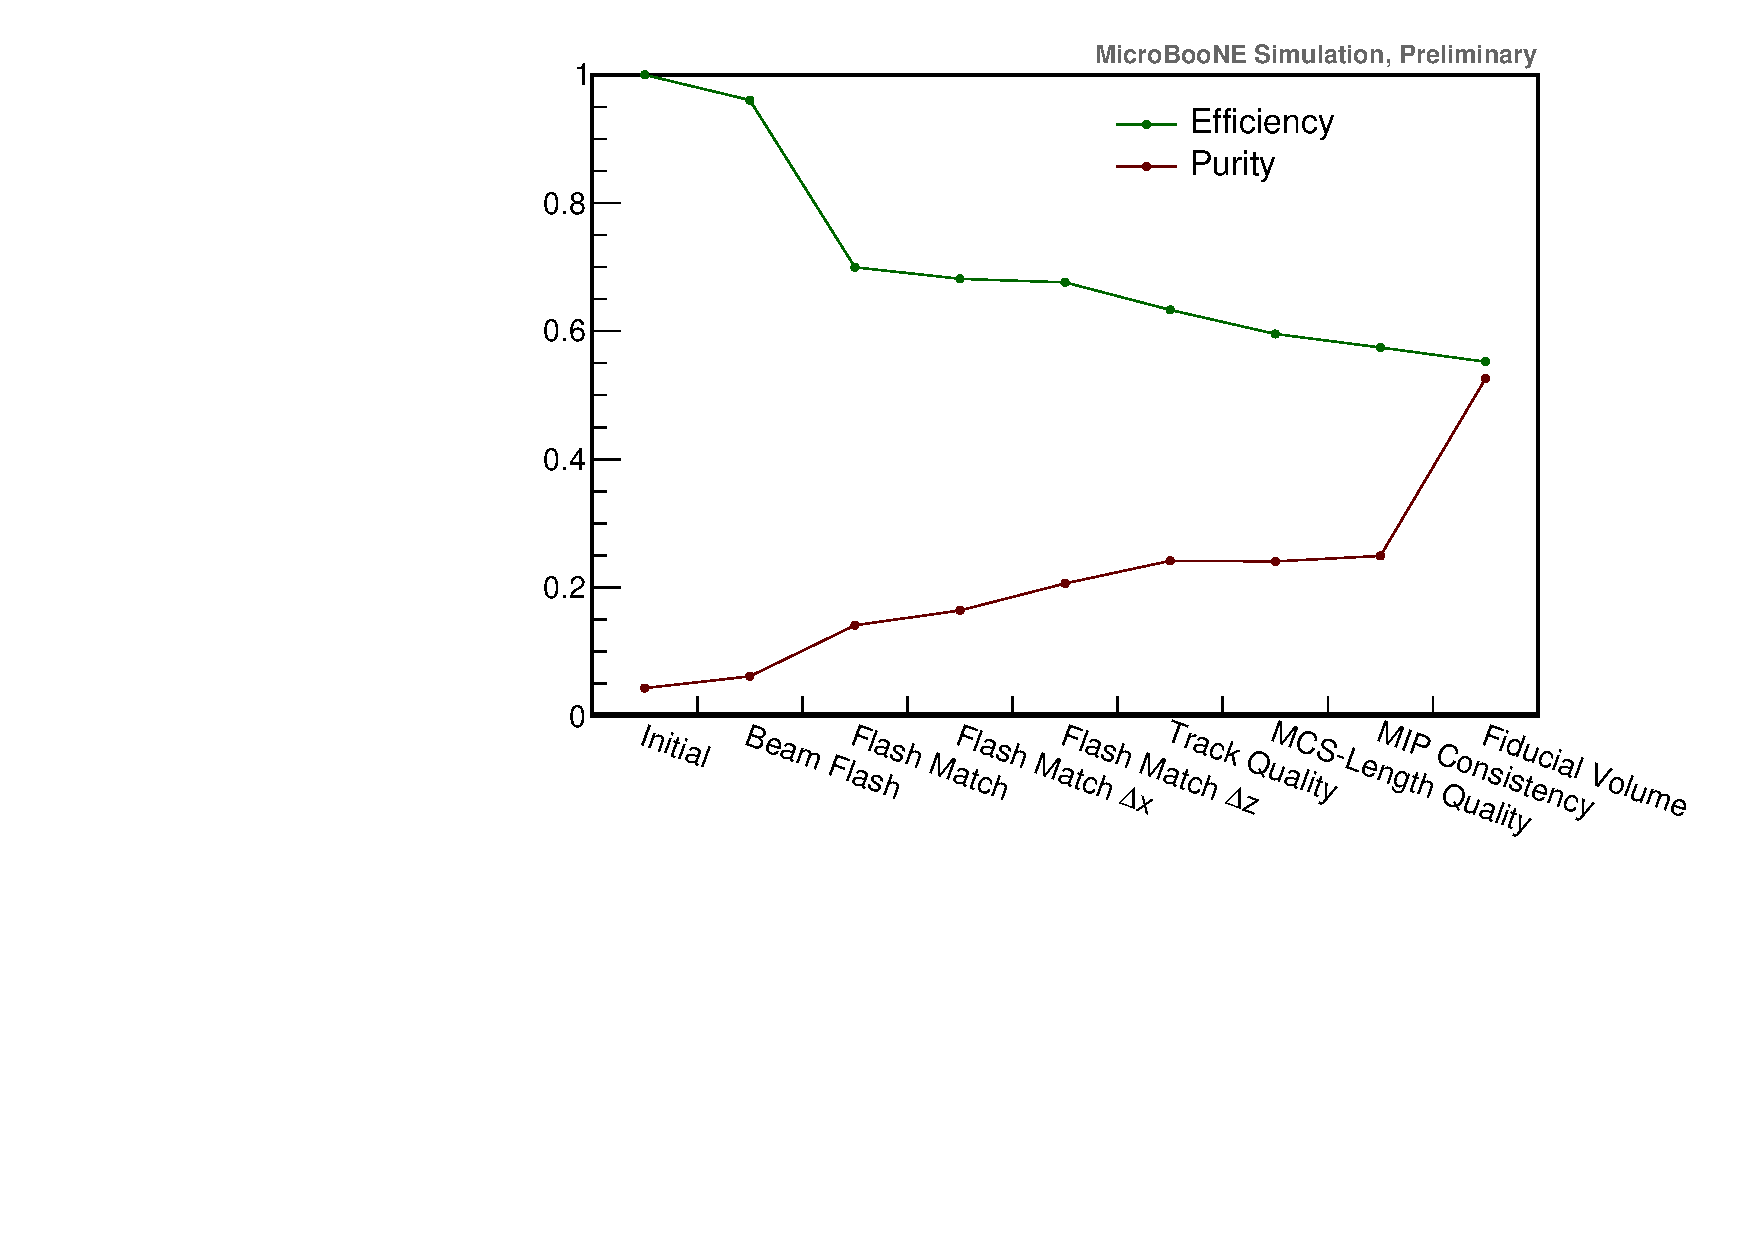
\includegraphics[width=.65\textwidth]{images/EfficiencyPlots/eff_pur_graph_percut}
%\caption{ Efficiency and purity as a function of the event selection cuts. The purity has been calculated by taking into account events from \extbnb data as well as events from \bnbcosmic \acrshort{mc}. Plot done with old selection, will be updated later.}
%\label{fig:eff_pur_graph_percut}
%\end{SCfigure}




\begin{figure}[]
\centering
\subfloat[][]
   {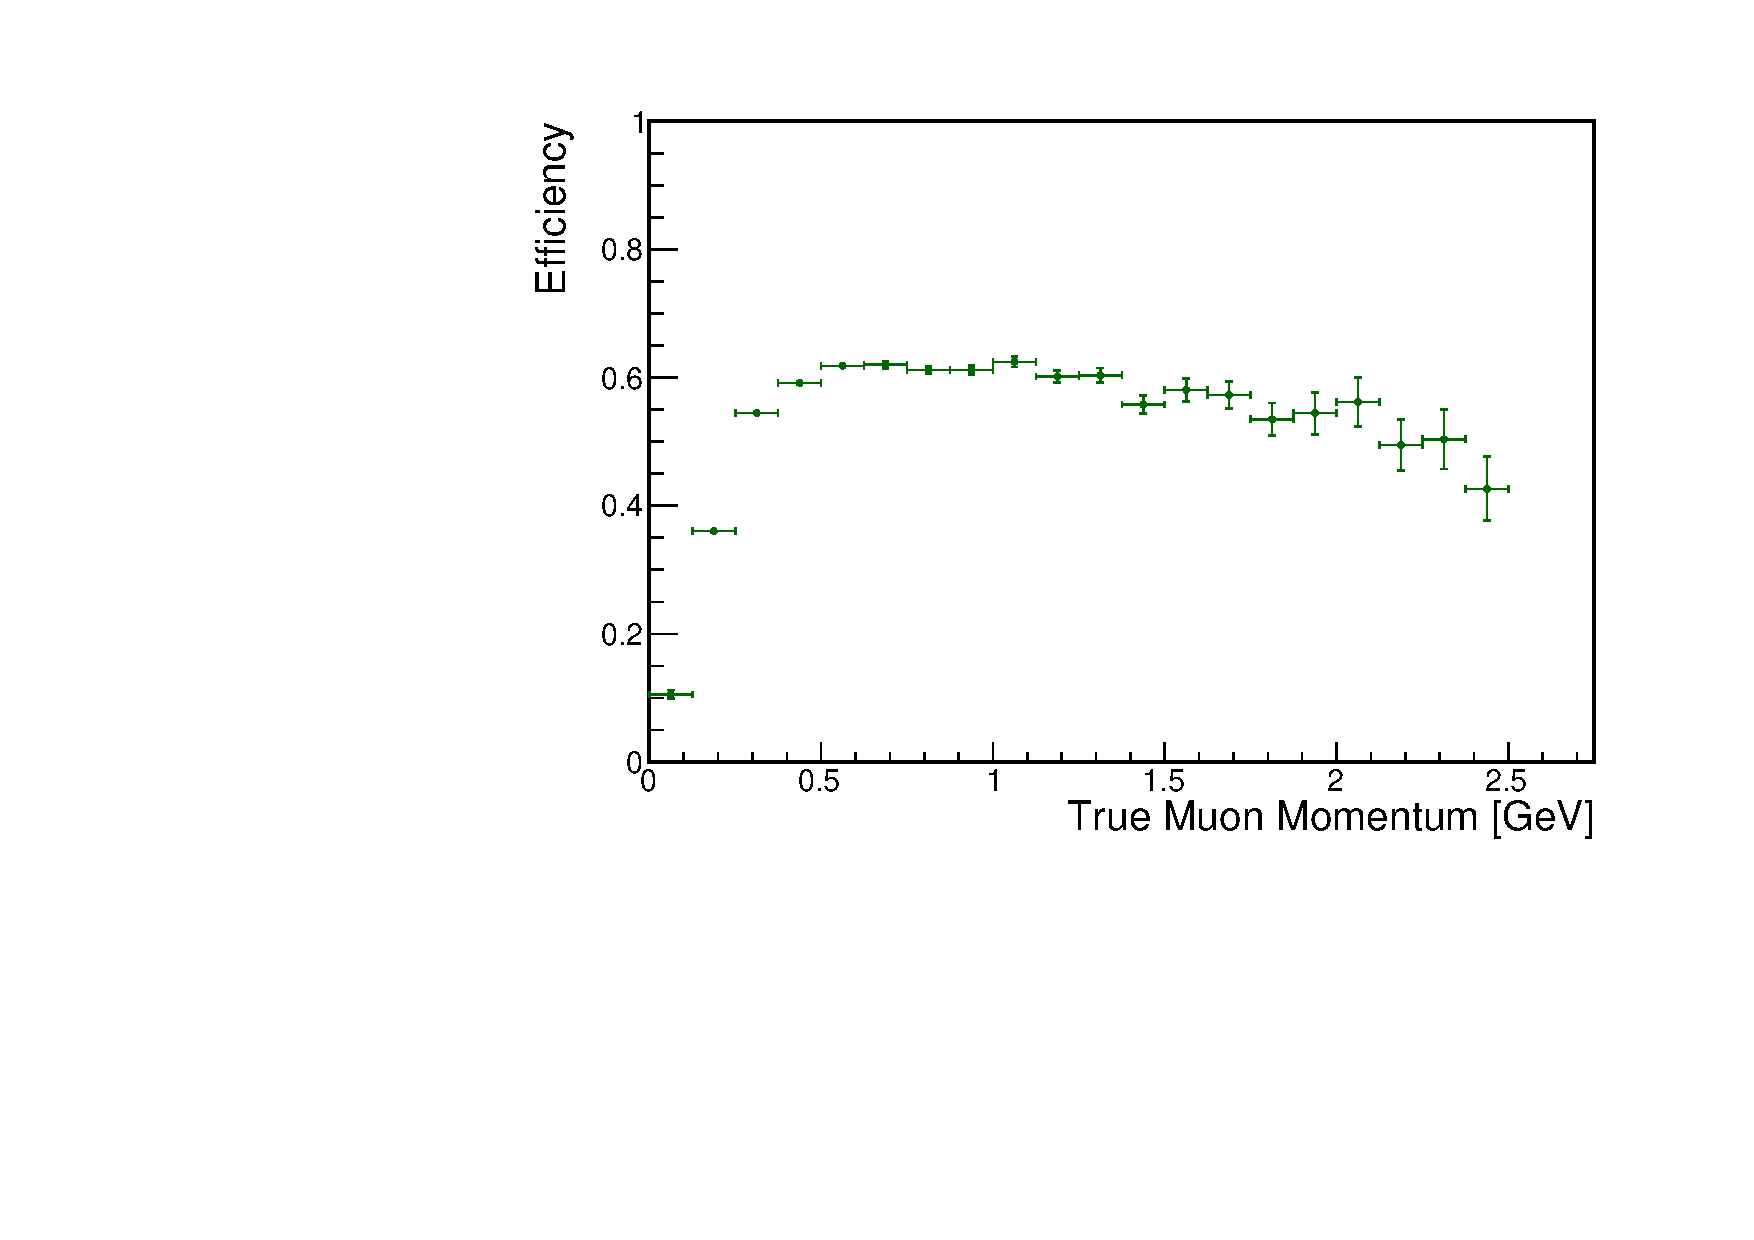
\includegraphics[width=.45\textwidth]{images/EfficiencyPlots/efficiency_mumom}
   \label{fig:eff_mumom}} \quad
\subfloat[][]
   {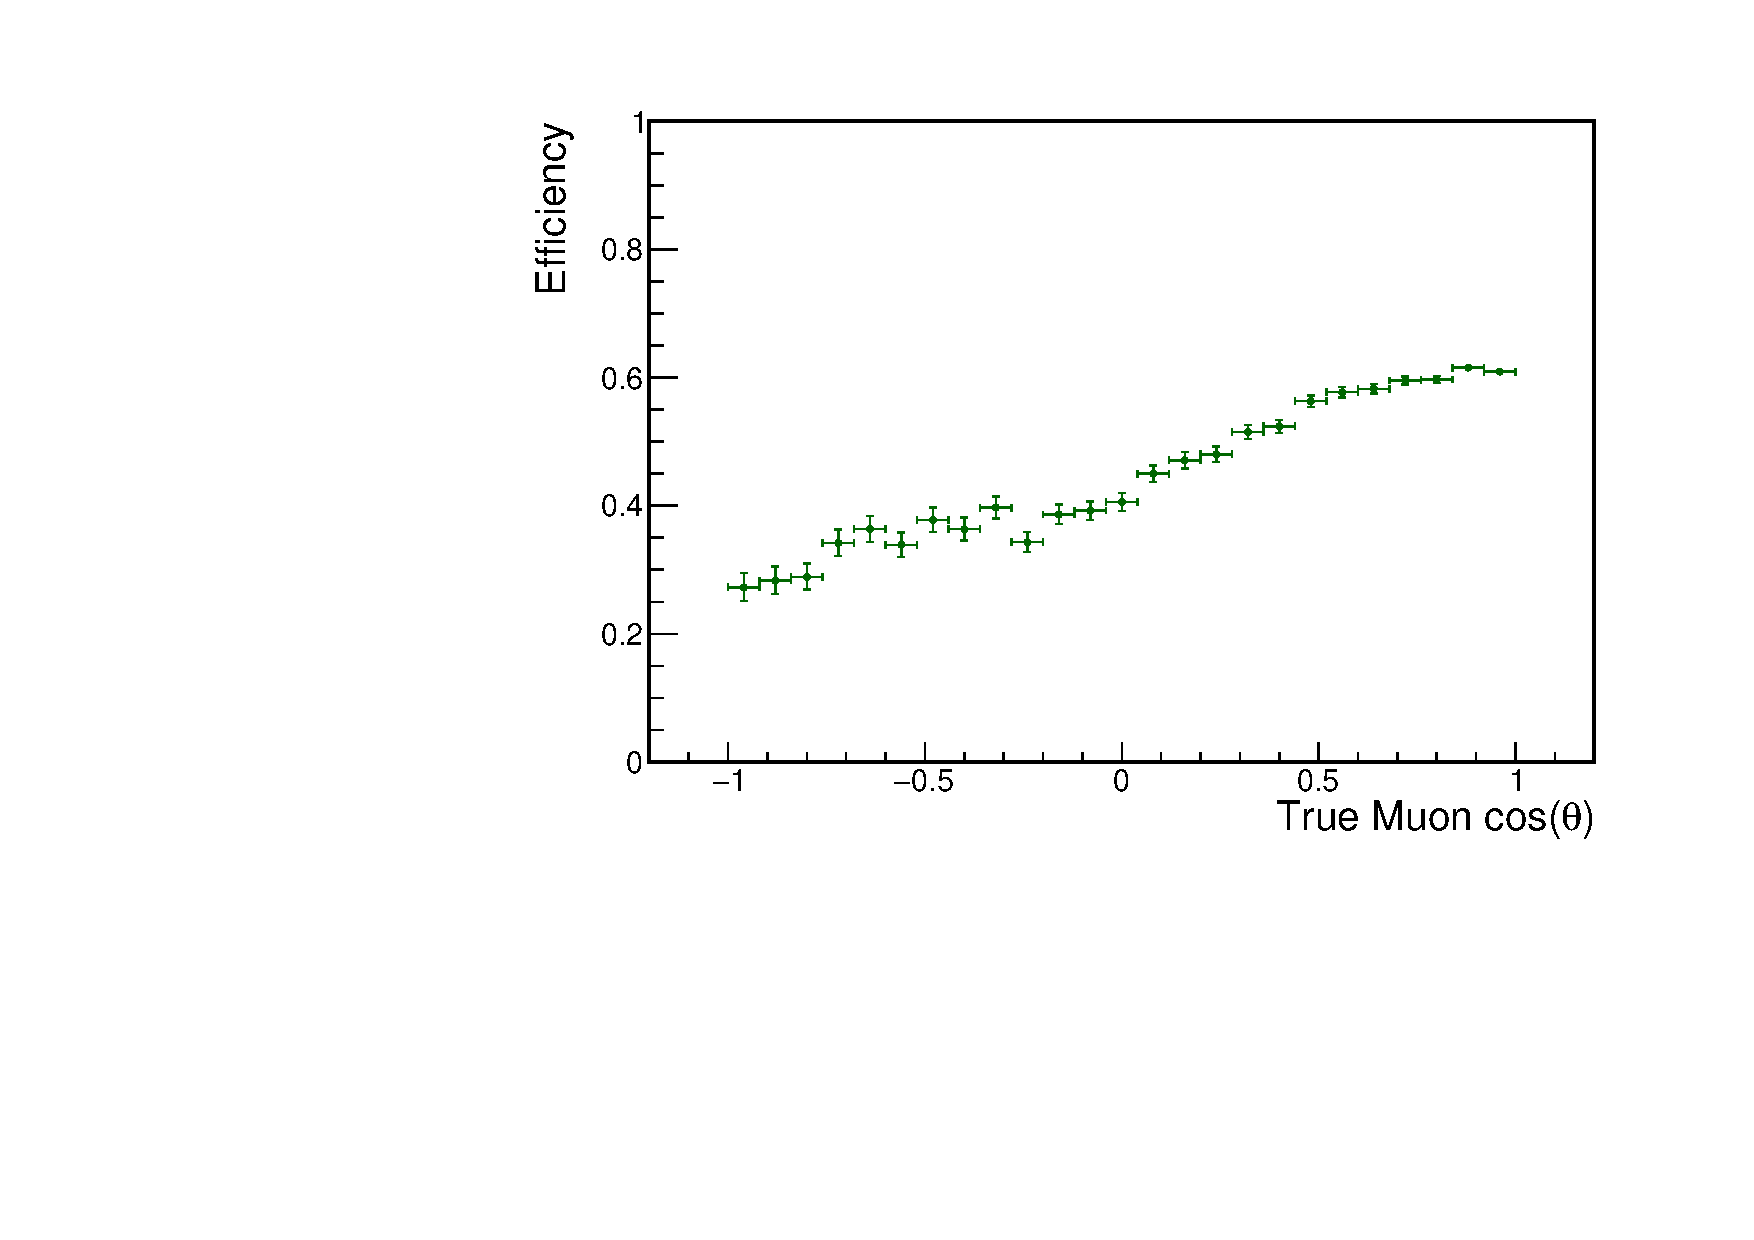
\includegraphics[width=.45\textwidth]{images/EfficiencyPlots/efficiency_muangle}
   \label{fig:eff_costheta}} \quad
\subfloat[][]
   {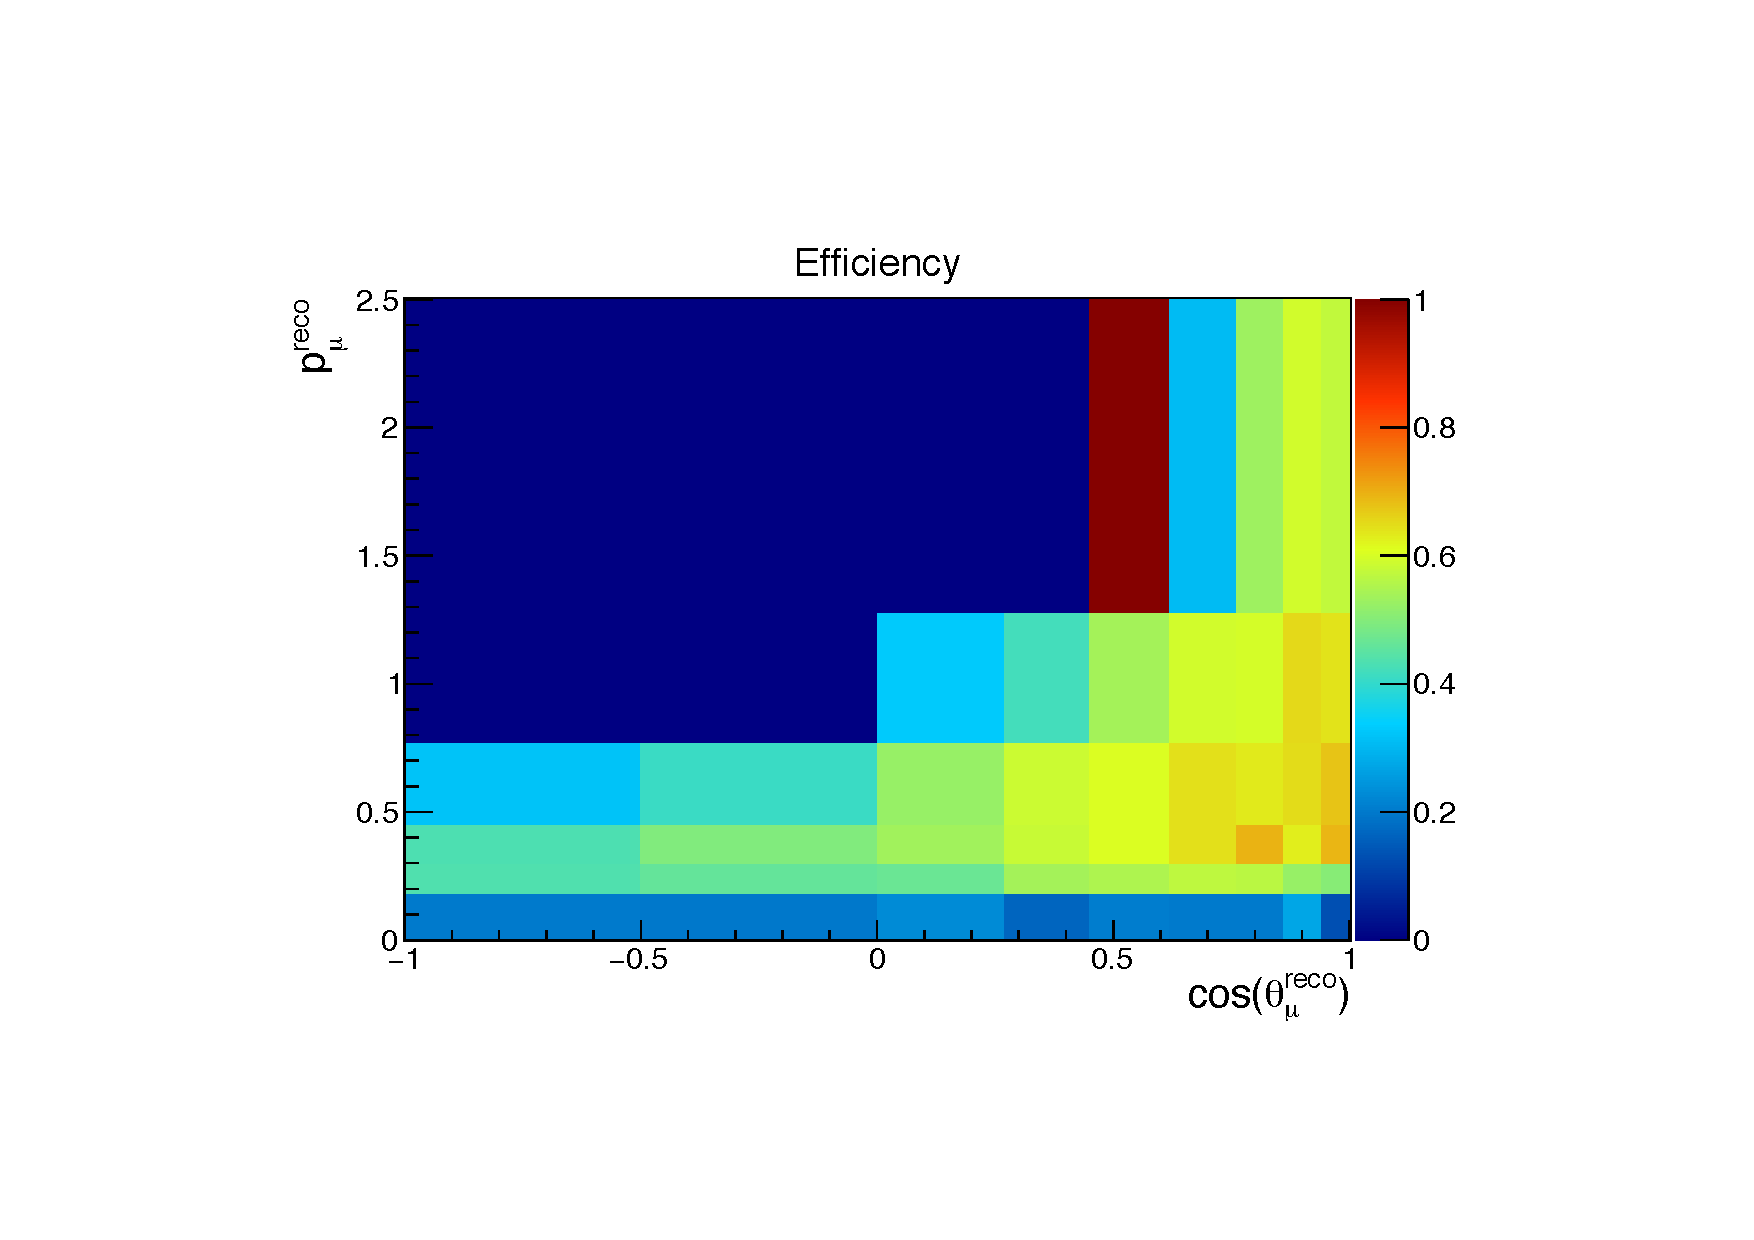
\includegraphics[width=.45\textwidth]{images/XSecPmuCosThetaMu/trkcostheta_trkmumom_efficiency_true_new}
   \label{fig:eff_mumom_costheta}} \quad
\subfloat[][]
   {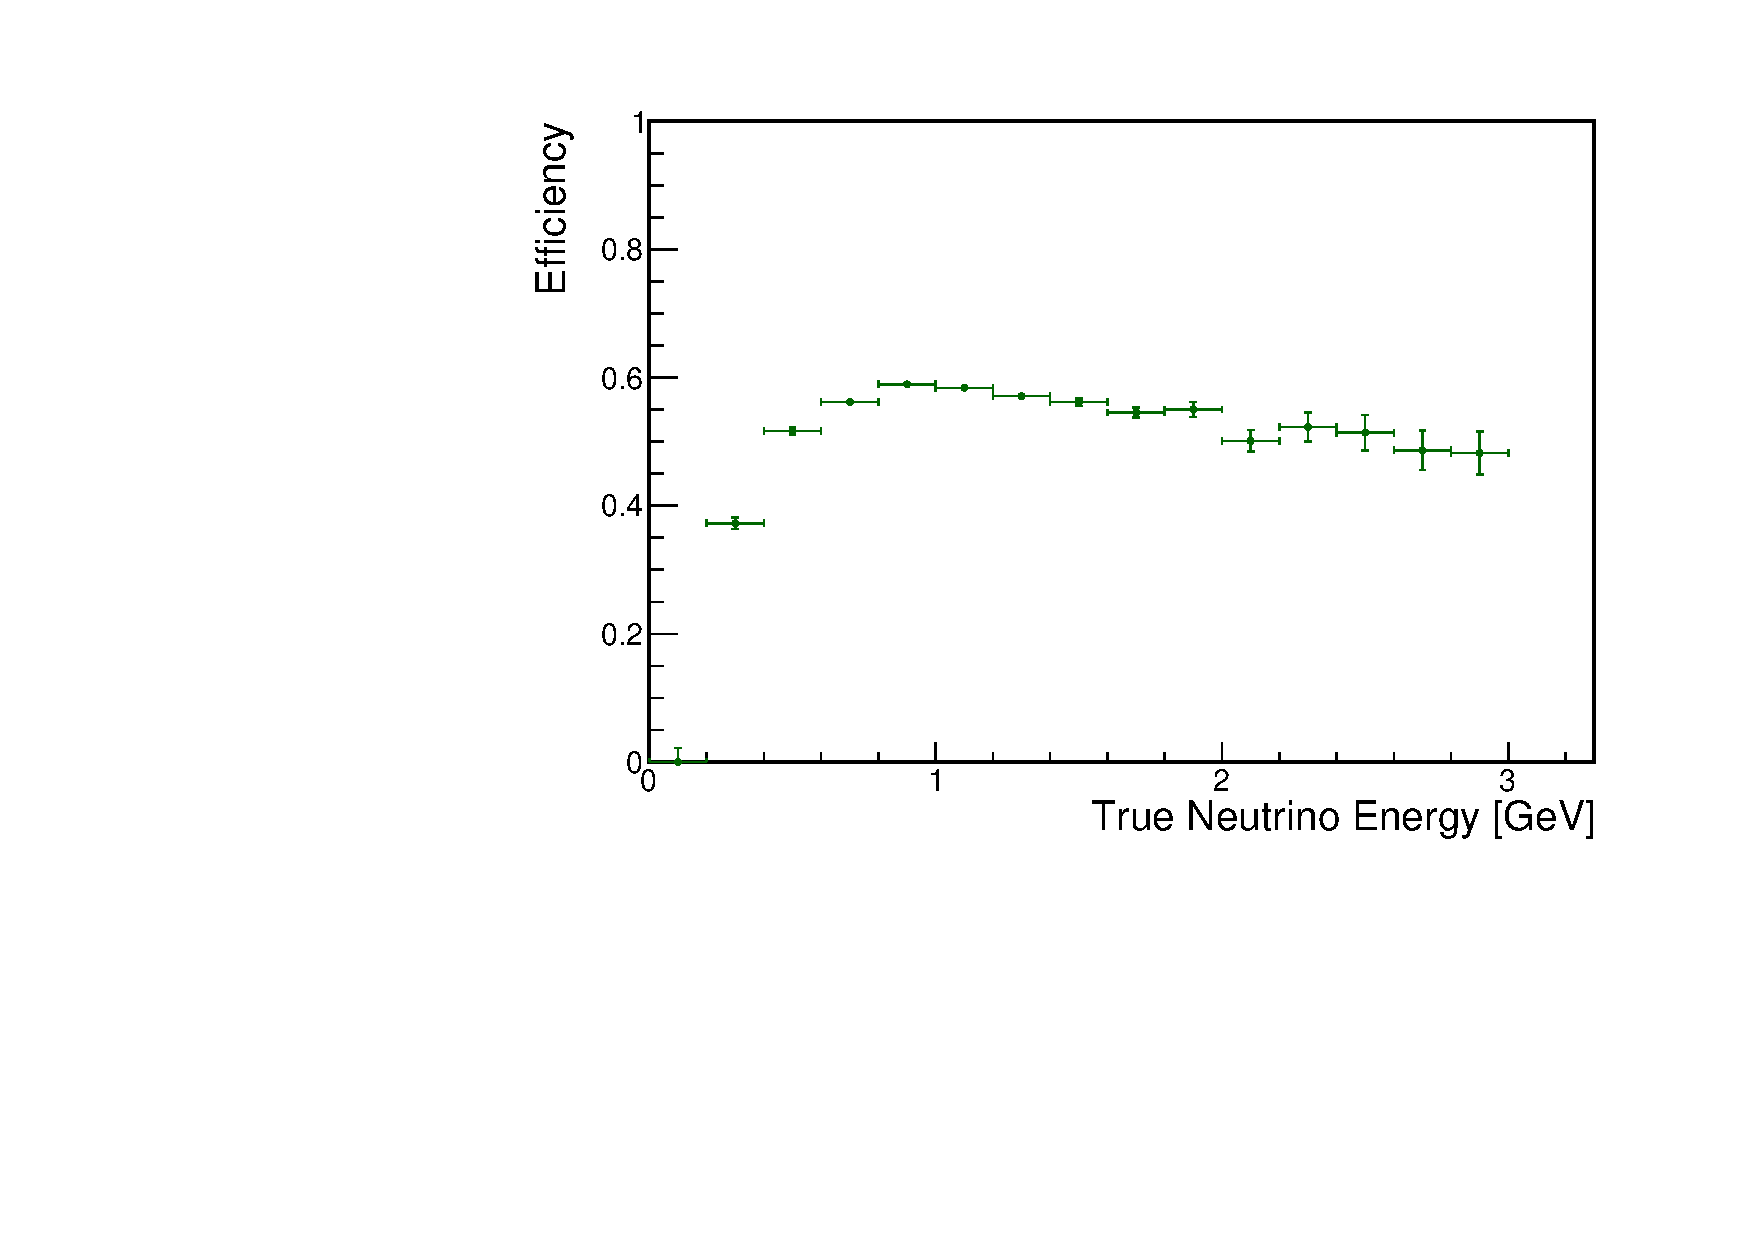
\includegraphics[width=.45\textwidth]{images/EfficiencyPlots/efficiency}
   \label{fig:efficiency}} \quad
\subfloat[][]
   {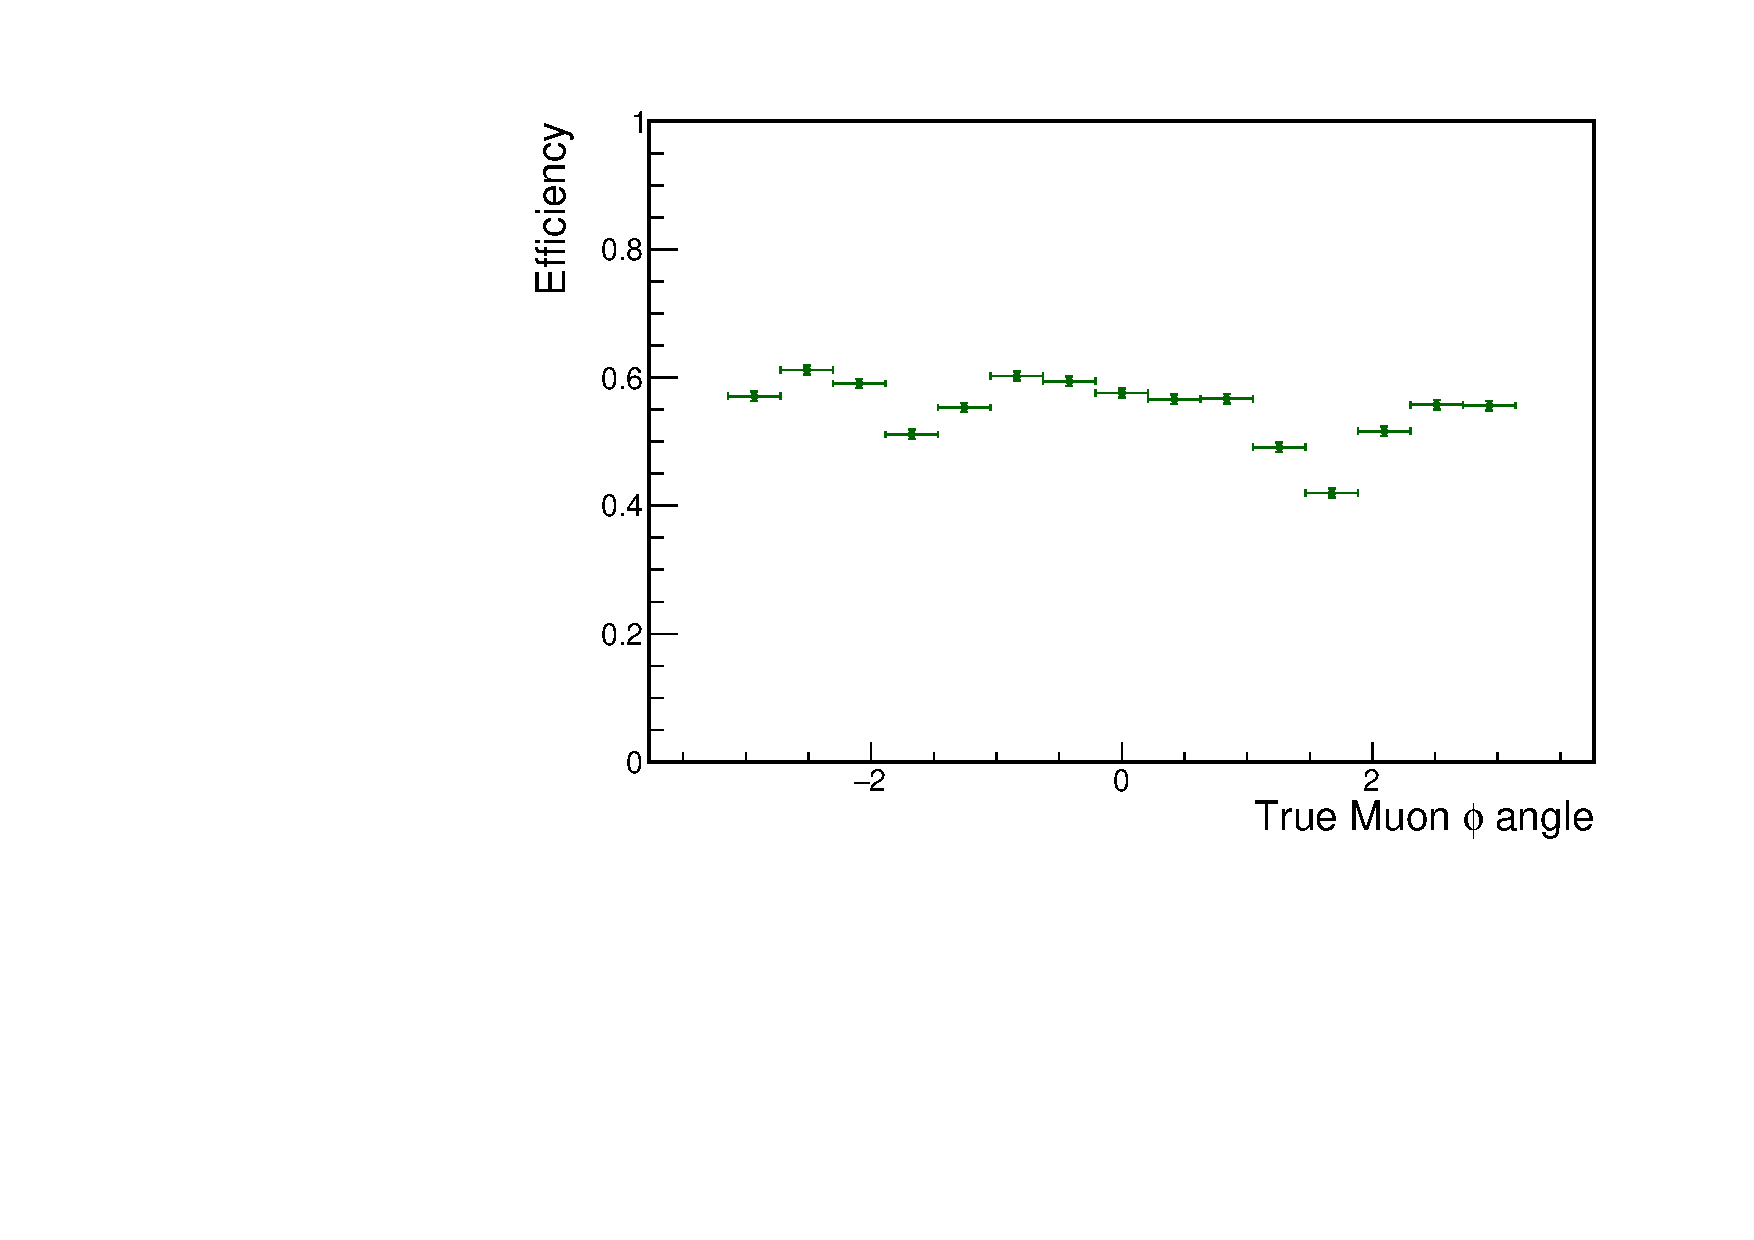
\includegraphics[width=.45\textwidth]{images/EfficiencyPlots/efficiency_muphi}
   \label{fig:eff_phi}} \quad
\subfloat[][]
   {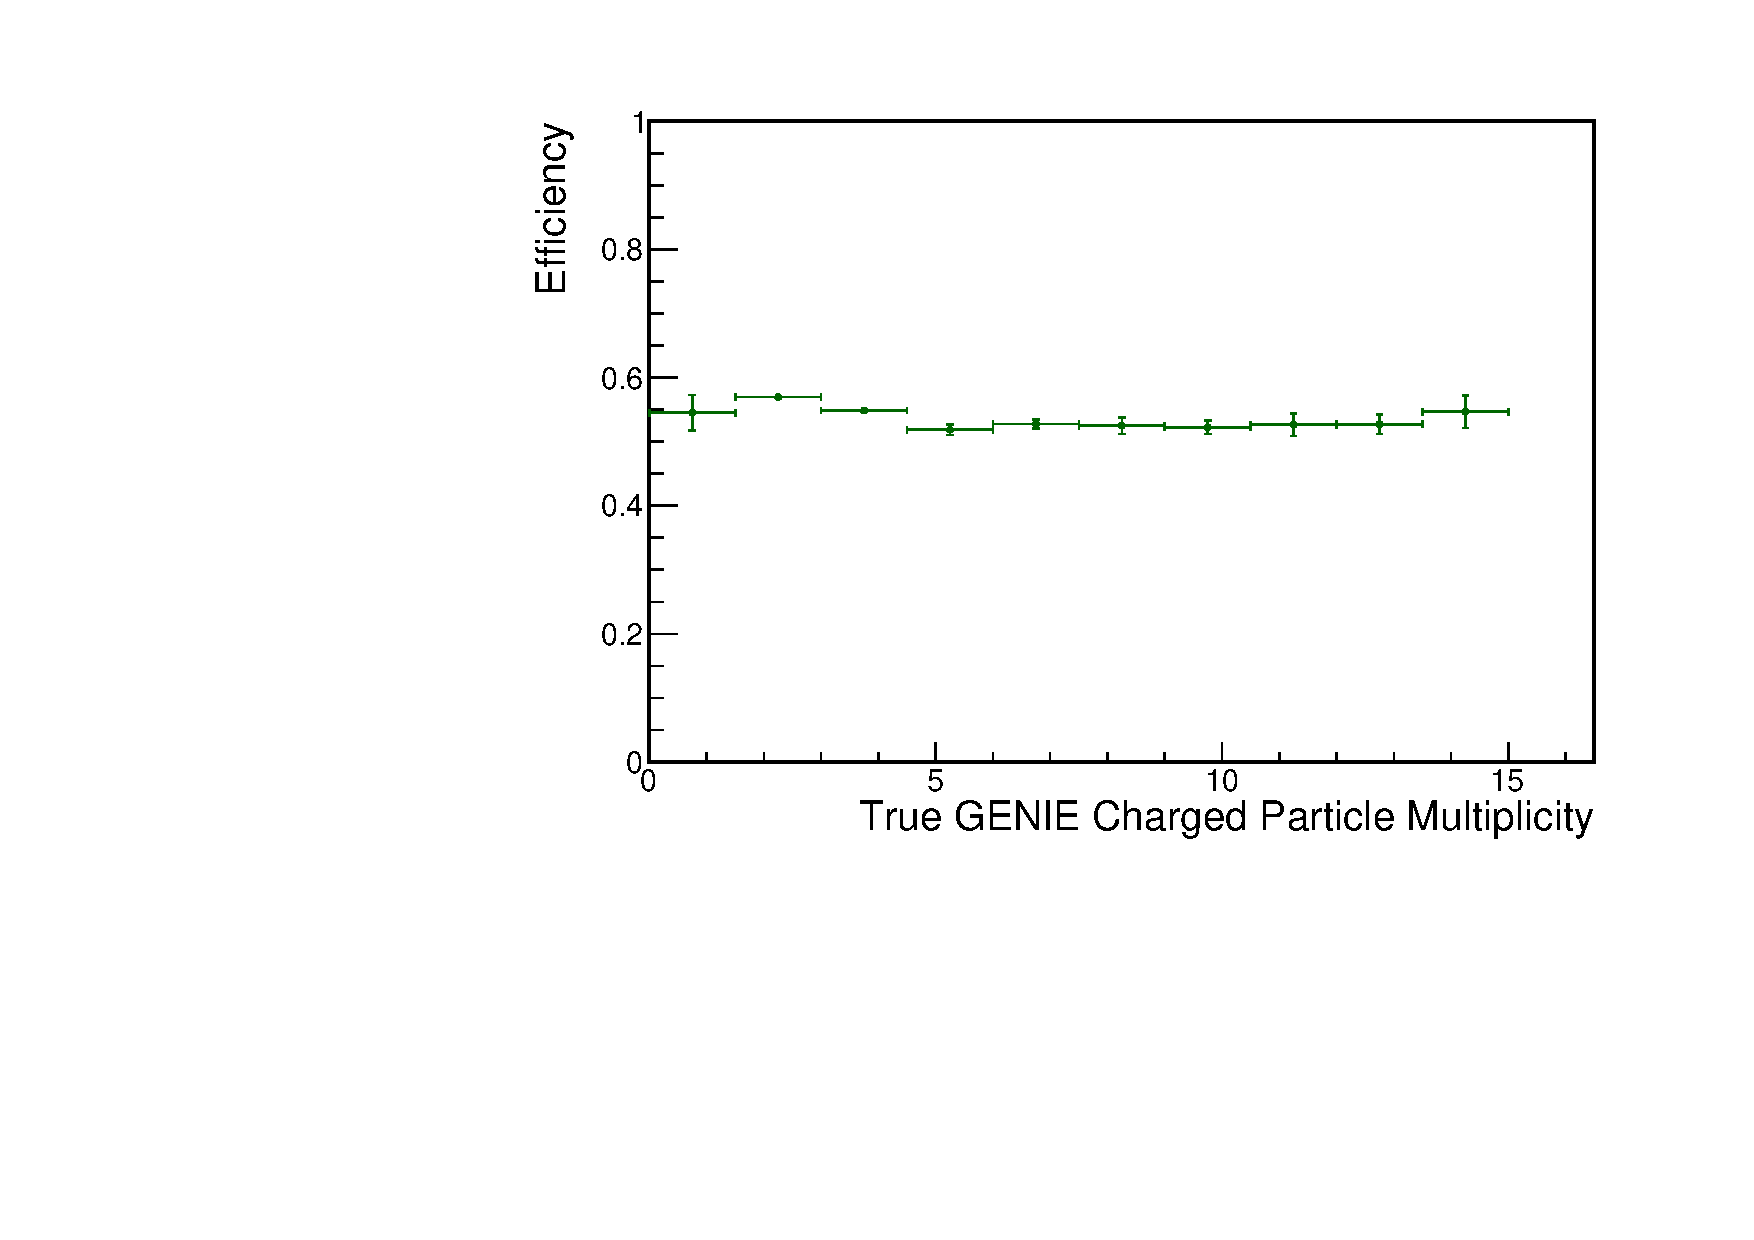
\includegraphics[width=.45\textwidth]{images/EfficiencyPlots/efficiency_mult_ch}
   \label{fig:eff_mult}} \\ 
\caption[Selection Efficiencies]{Final selection efficiency (efficiency $\times$ acceptance) as a function of the true muon momentum~\protect\subref{fig:eff_mumom}, cosine of the muon angle with respect to the beam~\protect\subref{fig:eff_costheta}, angle and momentum together~\protect\subref{fig:eff_mumom_costheta}, angle around the beam~\protect\subref{fig:eff_phi}, true initial neutrino energy~\protect\subref{fig:efficiency}, and true charged particle multiplicity~\protect\subref{fig:eff_mult} . The overall efficiency is 57.2\%.}
\label{fig:eff}
\end{figure}





Figure~\ref{fig:efficiency_mode} shows the efficiency as a function of true neutrino energy for the different \g interaction modes: \acrshort{qe}, resonance, \acrshort{dis} and \acrshort{mec}. There is also a negligible contribution from \acrshort{cc} coherent events not plotted. This plot shows that this event selection allows to select all the interaction modes, making this analysis really inclusive.


\begin{figure}[]
\centering
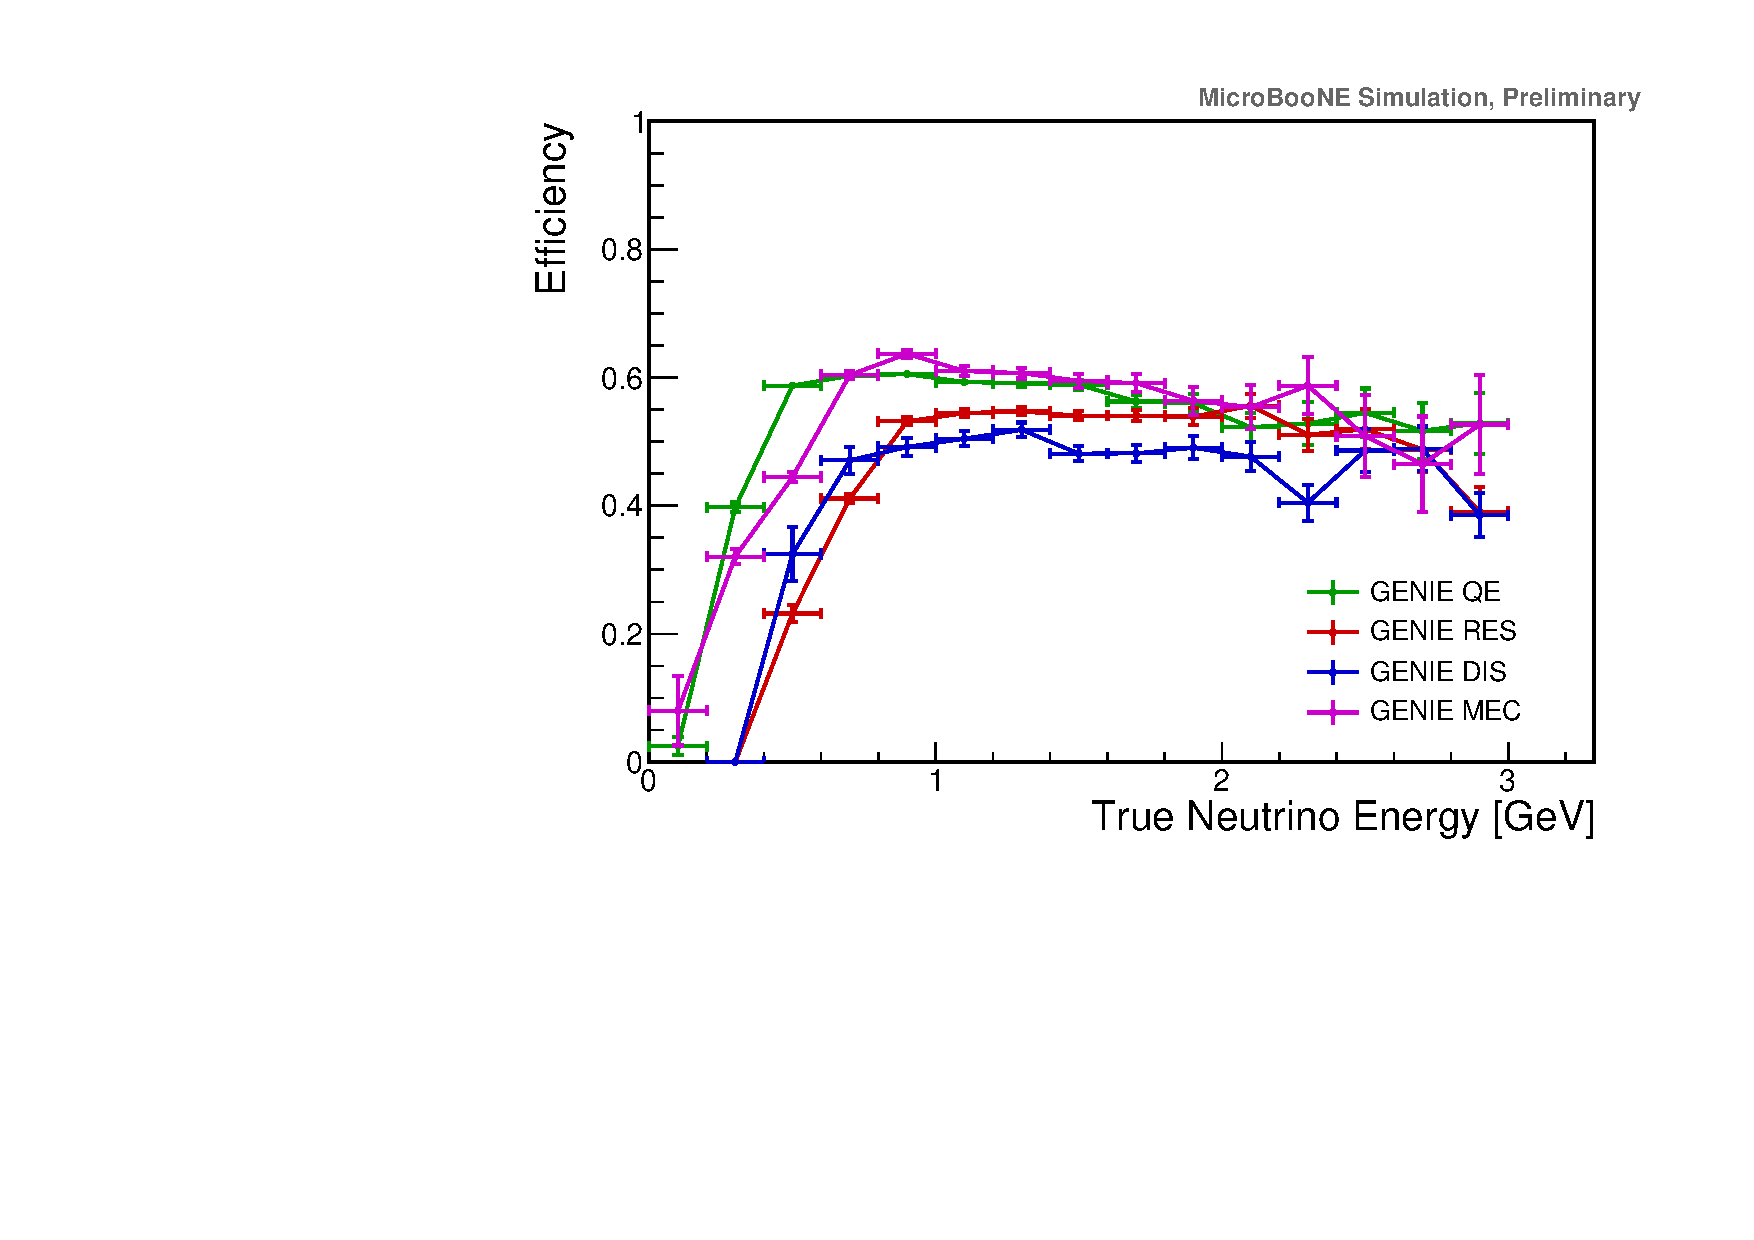
\includegraphics[width=.60\textwidth]{images/EfficiencyPlots/efficiency_mode}
\caption[Efficiency for Different Interaction Modes]{Efficiency as a function of true neutrino energy for different GENIE interaction modes. There is a negligible contribution from \acrshort{cc} coherent events not plotted.}
\label{fig:efficiency_mode}
\end{figure}


The plots in Figure~\ref{fig:mctruth_plots} show the distribution of true \g simulated variables: neutrino energy, muon momentum $p_\mu$, cosine of the muon polar angle $\cos\theta_\mu$, muon azimuthal angle $\phi$. These distribution are further divided in different \g interaction modes. Apart for a normalisation difference (the efficiency is $\sim$ 57\%), one can see that the distributions are not particularly shaped after the selection, so that the event selection is not introducing any particular bias.

\begin{figure}[t]
%\begin{adjustwidth}{-1cm}{-1cm}
\centering
\subfloat[][Generated.]
   {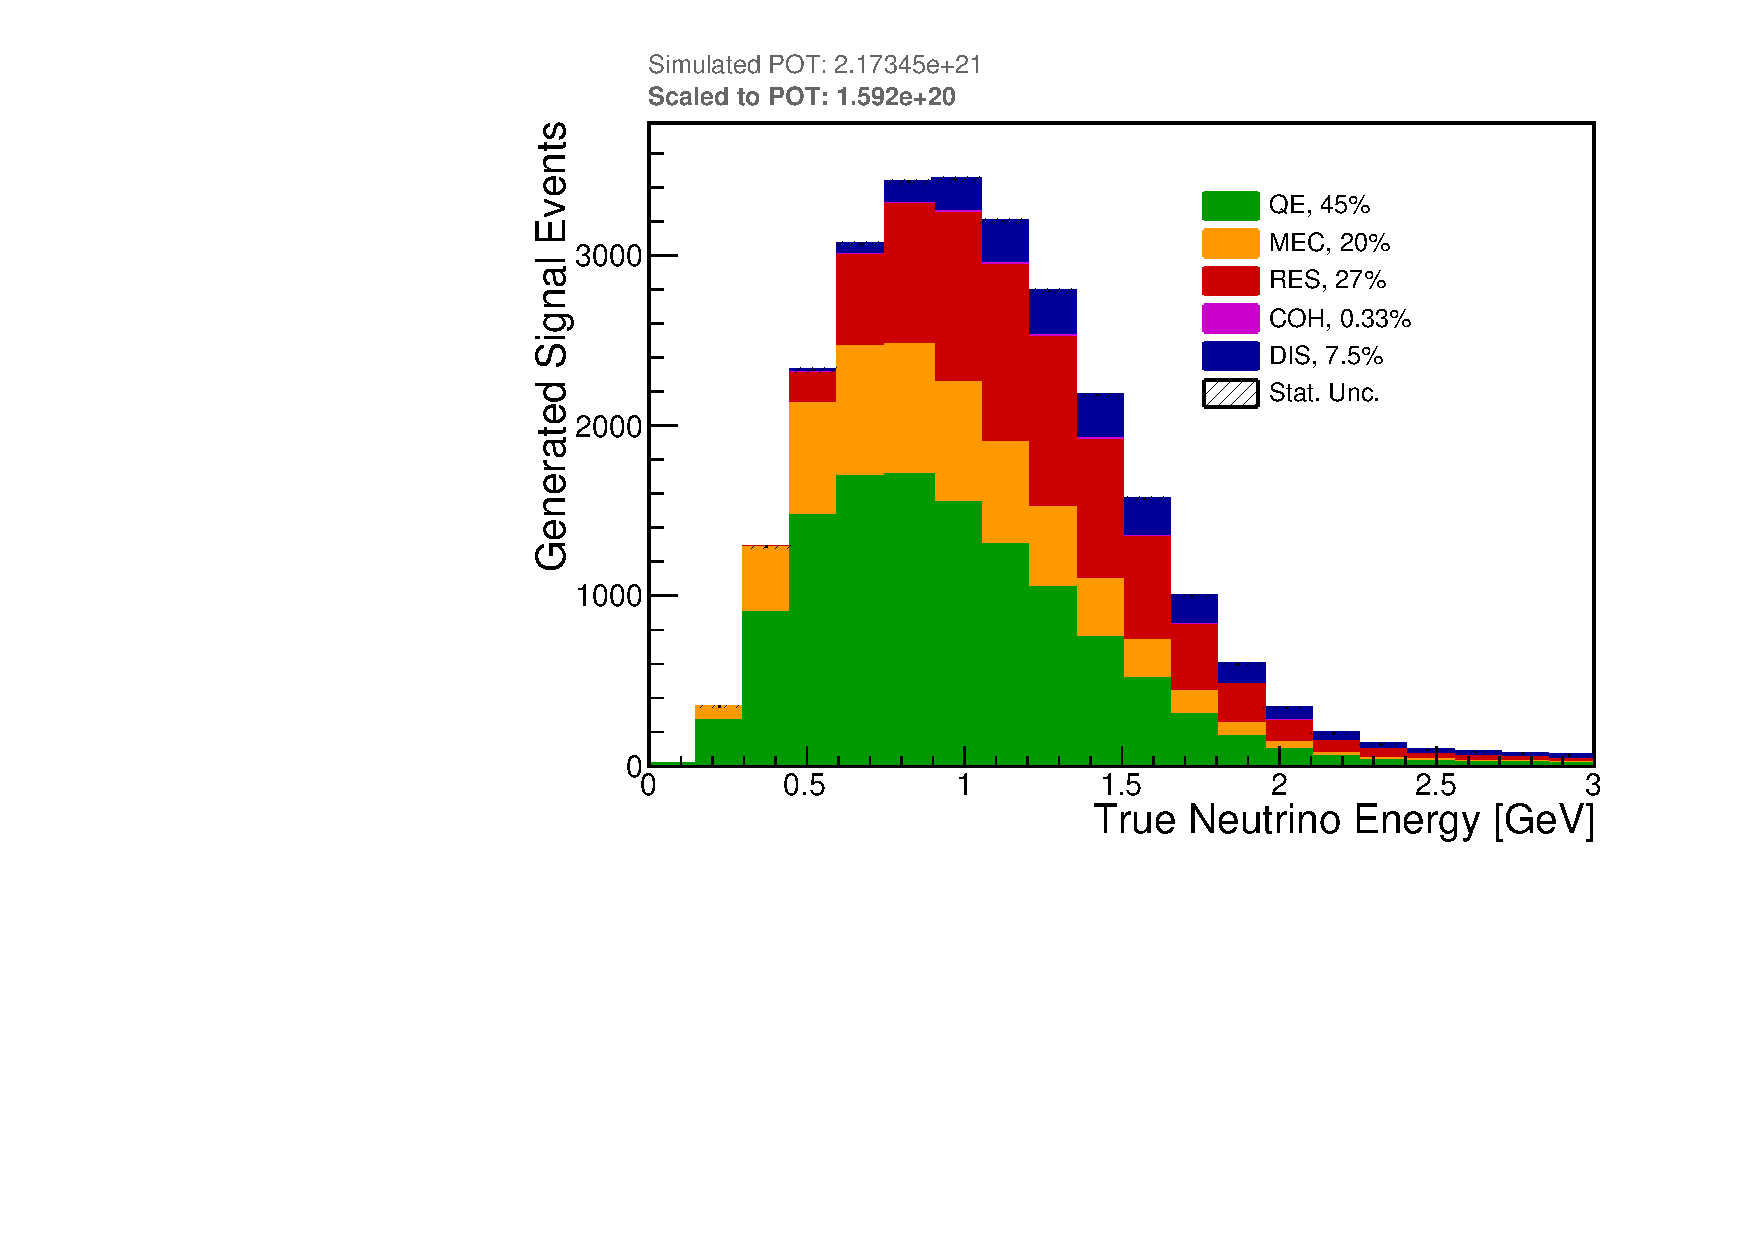
\includegraphics[width=.42\textwidth]{images/MCTruthPlots_Tune1/mctruth_nuenergy_gen}
   \label{fig:mctruth_nuenergy_gen}} \quad
\subfloat[][Selected.]
   {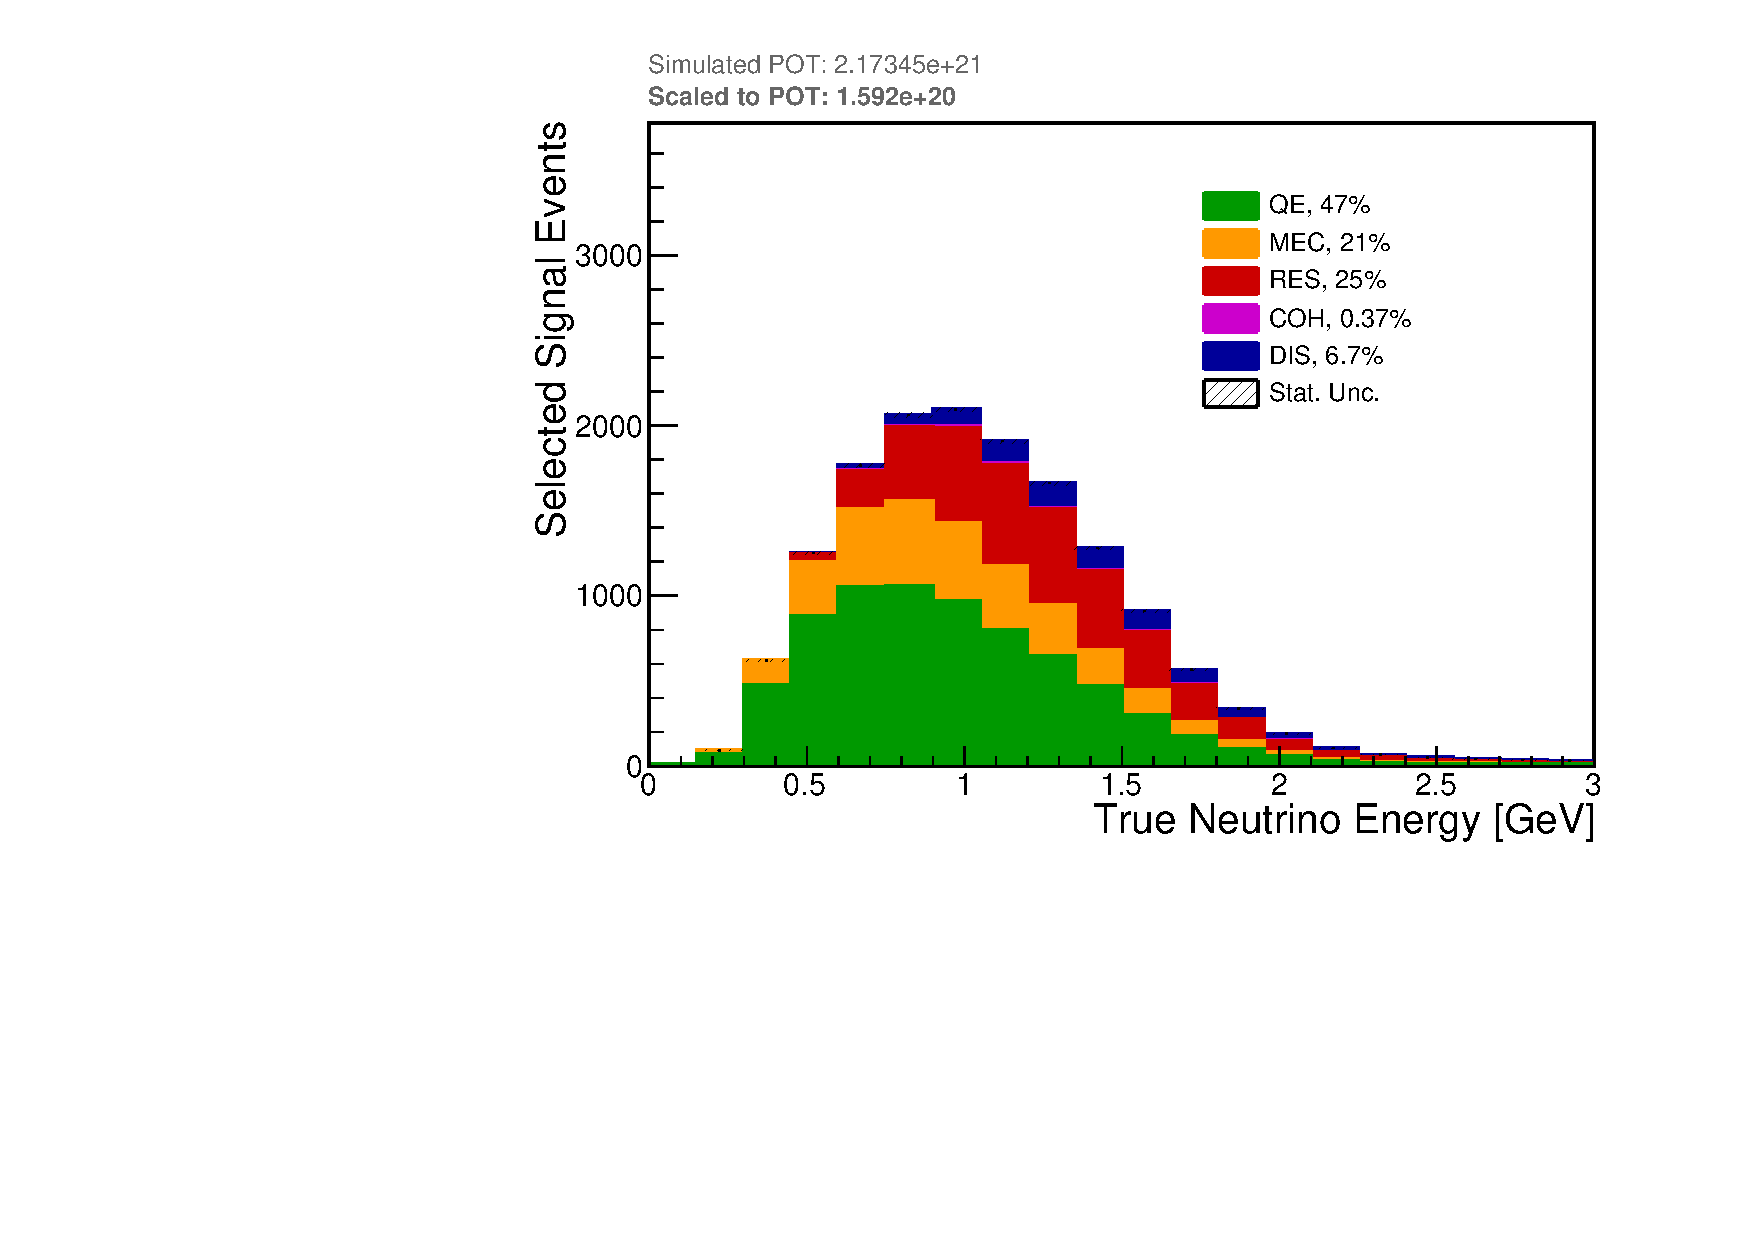
\includegraphics[width=.42\textwidth]{images/MCTruthPlots_Tune1/mctruth_nuenergy_sel}
   \label{fig:mctruth_nuenergy_sel}} \quad
\subfloat[][Generated.]
   {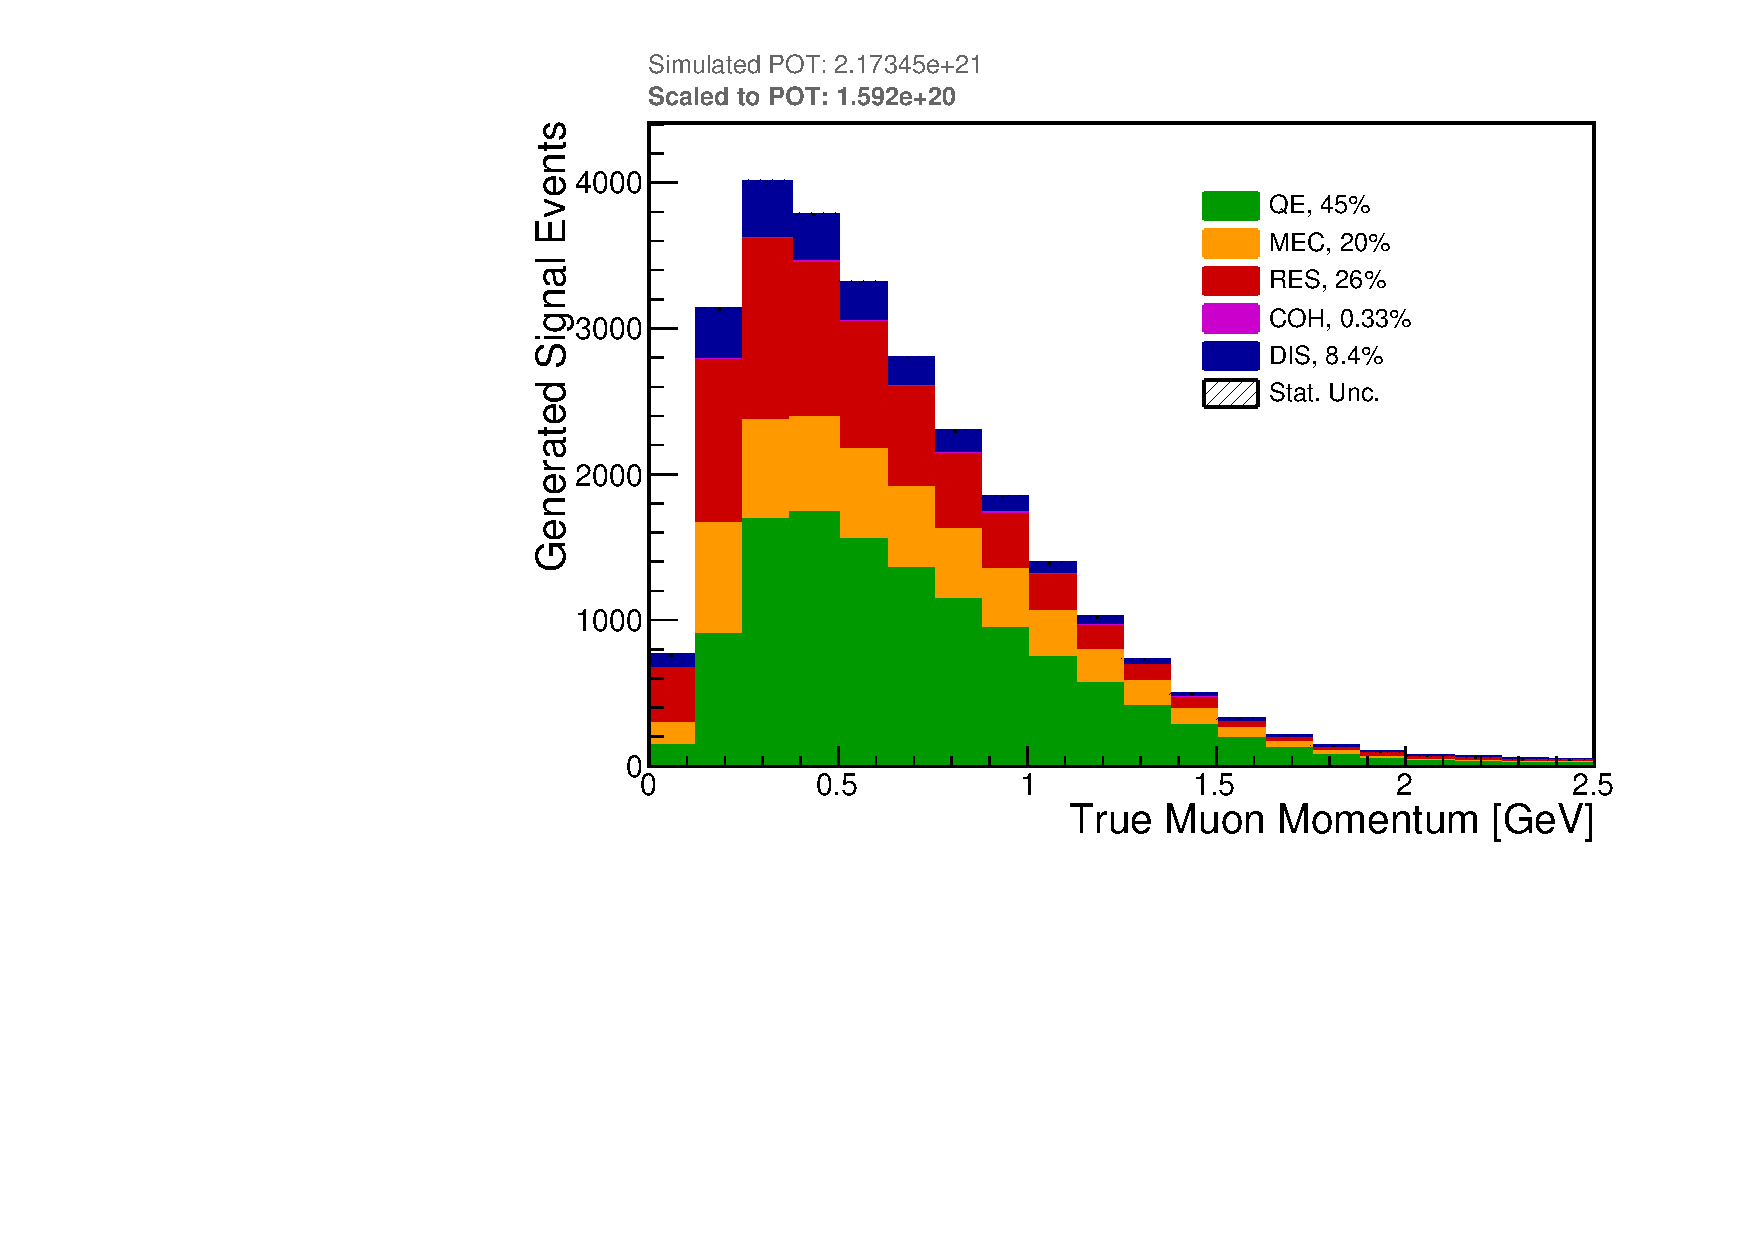
\includegraphics[width=.42\textwidth]{images/MCTruthPlots_Tune1/mctruth_mumom_gen}
   \label{fig:mctruth_mumom_gen}} \quad
\subfloat[][Selected.]
   {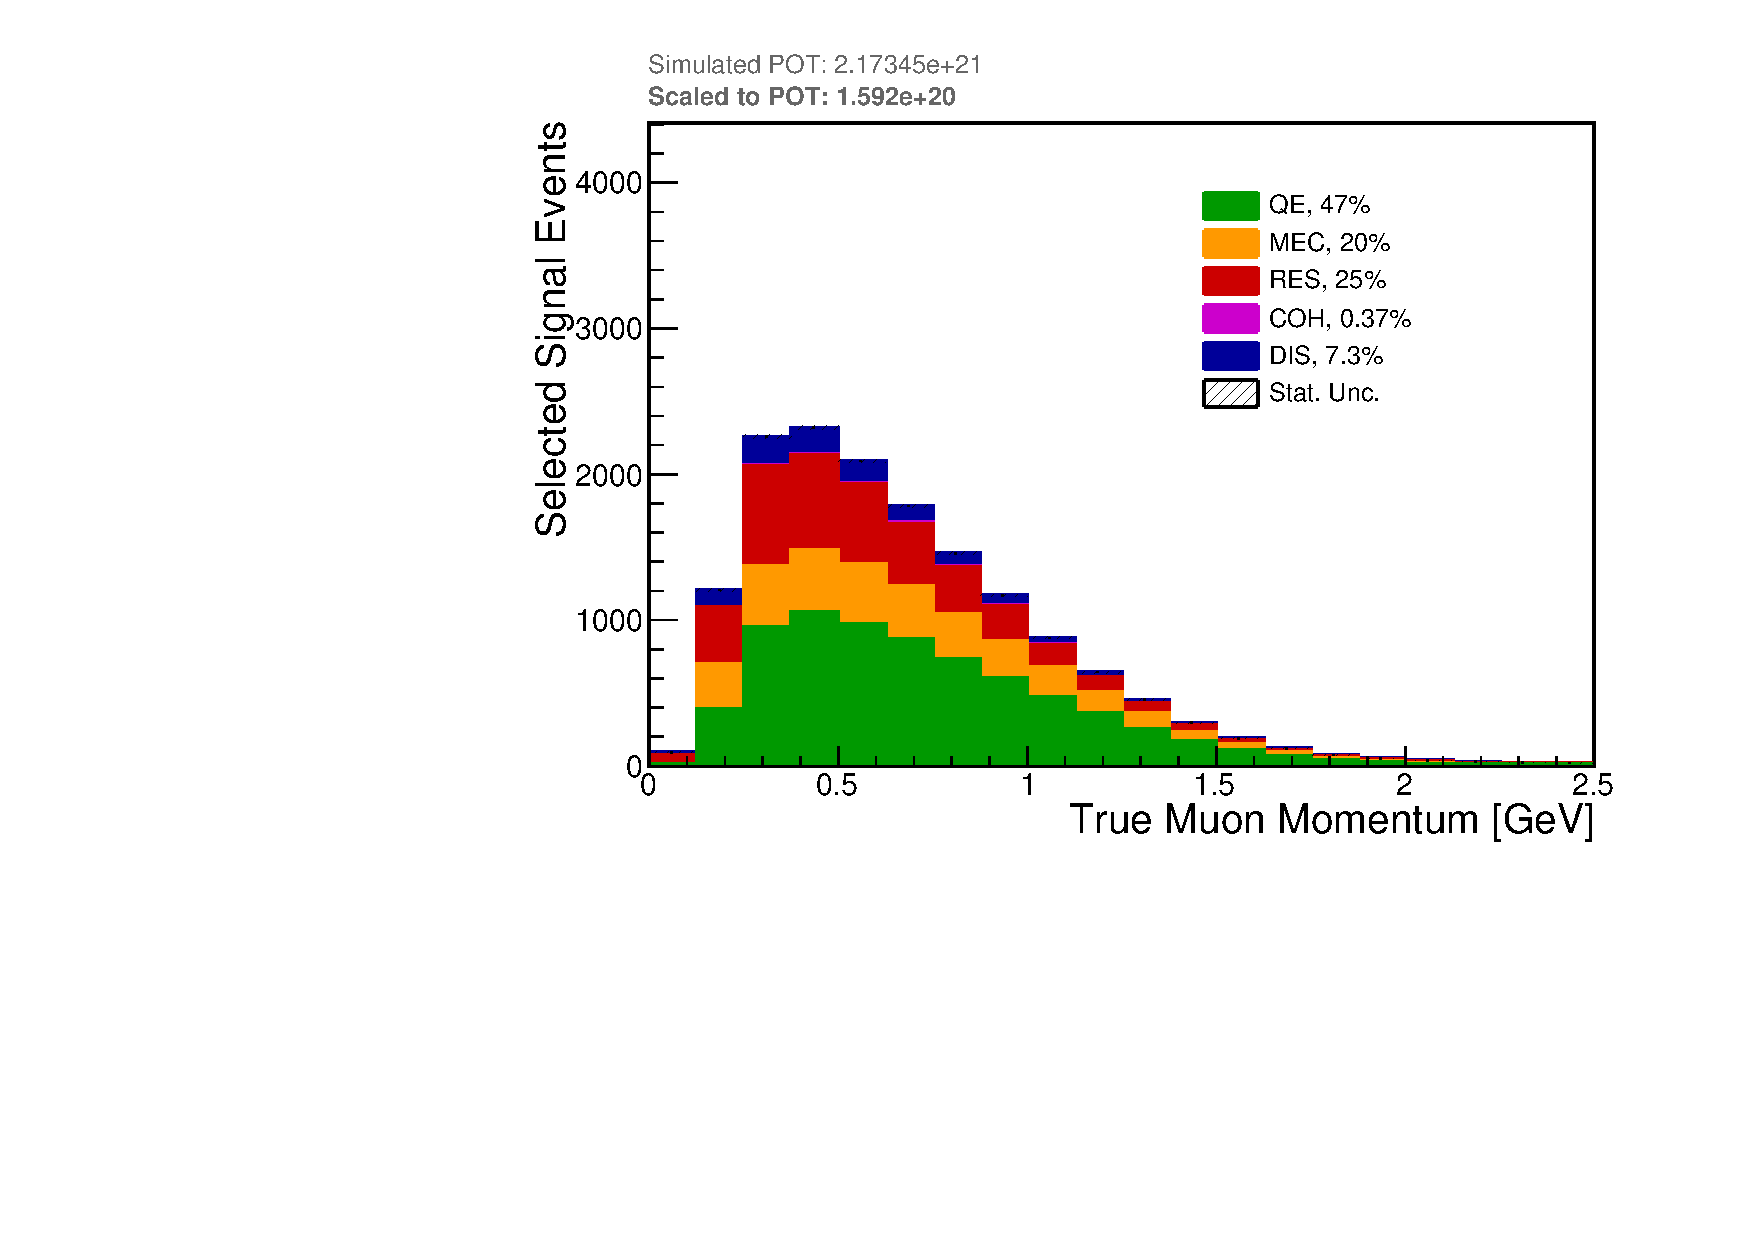
\includegraphics[width=.42\textwidth]{images/MCTruthPlots_Tune1/mctruth_mumom_sel}
   \label{fig:mctruth_mumom_sel}} \quad
\subfloat[][Generated.]
   {\includegraphics[width=.42\textwidth]{images/MCTruthPlots_Tune1/mctruth_mucostheta_gen}
   \label{fig:mctruth_mucostheta_gen}} \quad
\subfloat[][Selected.]
   {\includegraphics[width=.42\textwidth]{images/MCTruthPlots_Tune1/mctruth_mucostheta_sel}
   \label{fig:mctruth_mucostheta_sel}} \quad
\subfloat[][Generated.]
   {\includegraphics[width=.42\textwidth]{images/MCTruthPlots_Tune1/mctruth_muphi_gen}
   \label{fig:mctruth_muphi_gen}} \quad
\subfloat[][Selected.]
   {\includegraphics[width=.42\textwidth]{images/MCTruthPlots_Tune1/mctruth_muphi_sel}
   \label{fig:mctruth_muphi_sel}} \quad
\caption[Simulated Variables Distributions Before and After Selection]{Distributions of true variables for generated (left) and selected (right) signal events ($\nu_\mu$ \acrshort{cc} in \acrshort{fv}). These plots have been made with a $8.9 \times 10^{20}$ equivalent \acrshort{pot} \acrshort{mc}. They have then been scaled to $1.6\times 10^{20}$ \acrshort{pot}, which are the data \acrshort{pot} used for this analysis. The coloured histogram are stacked. The distributions are generated with the  ``\tuneone'' configuration.}
\label{fig:mctruth_plots}
%\end{adjustwidth}
\end{figure}






\section{Event Selection Summary}

This chapter described the event selection used to select $\nu_\mu$ \acrshort{cc} events in the \acrshort{fv}. The overall selection efficiency is 57.2\%, with a purity of 50.4\%. These performances have been estimated by looking at the ``\tuneone'' configuration, which is the MicroBooNE baseline simulation. The main background is due to \acrshort{cr} only events (for which a data driven estimate using beam-off data is used) and from events where neutrino interactions are present, but a \acrshort{cr} in the same event is selected (estimated using simulation). The second main background is caused by neutrino interactions outside the \acrshort{fv}. The next chapter will use events passing this selection to perform a cross section measurement.


